\documentclass[oneside]{book}
\usepackage[a4paper, total={6in, 8in}]{geometry}
\usepackage[english]{babel}
\usepackage[utf8]{inputenc}
\usepackage[T1]{fontenc}
\usepackage{cancel}
\usepackage{amsmath}
\usepackage{amsfonts}
\usepackage{listings}
\usepackage{hyperref}
\usepackage{siunitx}
\usepackage{fancyhdr}
\usepackage{textcomp}
\usepackage{makecell}
\usepackage[font=small,labelfont=bf]{caption}
\usepackage{pdfpages}
\usepackage{multicol}
\usepackage[ruled,vlined]{algorithm2e}
\usepackage{soul}
\usepackage{mhchem}
\usepackage[toc, page]{appendix}
\usepackage{float}
\usepackage{wrapfig}
\usepackage{braket}
\usepackage{xcolor}
\pagestyle{fancy}
\fancyhf{}
\lhead{\rightmark}
\cfoot{\leftmark}
\rfoot{\thepage}

\setcounter{secnumdepth}{5}

\lstset{
    frame=tb, % draw a frame at the top and bottom of the code block
    tabsize=4, % tab space width
    showstringspaces=false, % don't mark spaces in strings
    numbers=none, % display line numbers on the left
    commentstyle=\color{green}, % comment color
    keywordstyle=\color{red}, % keyword color
    stringstyle=\color{blue}, % string color
    breaklines=true,
    postbreak=\mbox{\textcolor{green}{$\hookrightarrow$}\space}
}

\renewcommand{\lstlistingname}{}% Listing -> Algorithm
\renewcommand{\lstlistlistingname}{Algoritmi}% List of Listings -> List of Algorithms
\author{
  Giacomo Fantoni \\
  \small Telegram: \href{https://t.me/GiacomoFantoni}{@GiacomoFantoni} \\[3pt]
  Github: \href{https://github.com/giacThePhantom/AlgoritmiStruttureDati}{https://github.com/giacThePhantom/AlgoritmiStruttureDati}}


\renewcommand*{\listalgorithmcfname}{}
\renewcommand*{\algorithmcfname}{}
\renewcommand*{\algorithmautorefname}{}
\renewcommand{\thealgocf}{}
\newcommand{\mathcolorbox}[2]{\colorbox{#1}{$\displaystyle #2$}}


\title{\Huge \textbf{Molecular Physics}}

\author{
  Giacomo Fantoni \\
  \small Telegram: \href{https://t.me/GiacomoFantoni}{@GiacomoFantoni} \\[3pt]
  Ilaria Cherchi\\
  \small Telegram: \href{https://t.me/ilariacherchi}{@ilariacherchi} \\[3pt]
  Alessia Guadagnin\\
  \small Telegram: \href{https://t.me/alessiagp}{@alessiagp} \\[3pt]
  Elisa Pettin\`a\\
  \small Telegram: \href{https://t.me/elisapettina}{@elispettina} \\[3pt]
  Stefano Cretti\\
  \small Telegram: \href{https://t.me/StefanoCretti}{@StefanoCretti} \\[3pt]
\small Github: \href{https://github.com/giacThePhantom/MolecularPhysics}{https://github.com/giacThePhantom/MolecularPhysics}}
\begin{document}
\maketitle
\tableofcontents

  \part{Quantum mechanics}

    \chapter{Revisiting classical mechanics}

\section{Physical theories}

  \subsection{Experiment}
  An experiment performed on a physical system is a way to measure observable quantities at a determined time: $O_1(t), \dots, O_n(t)$.
  By measuring more and more observables at the same time, the instantaneous state of the system becomes increasingly characterized.
  A maximum set of observables that leads to the complete characterization of the instantaneous state can be assumed.

    \subsubsection{Example - particle of mass $m$ subject to an harmonic force}
    A particle of mass $m$ subject to an harmonic force like one of a spring is completely characterized by:

    $$(\vec{r}(t),\vec{v}(t))=\vec{r}(t)\in \mathbb{R}^6$$

  \subsection{Definition}
  A physical theory is a mathematical scheme to predict the state of the system, the outcome of feature observations: $O_1(t'), \dots, O_n(t')$.
  In particular, an equation that can be used to compute the state at $t'$ given the state at $t$ is called an equation of motion.
  A physical theory is composed by the following elements:

  \begin{multicols}{2}
  \begin{itemize}
      \item definition of the state of a system
      \item recipe to determine the system's equation of motion
      \item prediction of an observable quantity given the state of the system
    \end{itemize}
  \end{multicols}


\section{Classical mechanics}
In classical mechanics, the state of a system is a collection at time $t$ of all the positions of all the particles in the system.
We also need to define the velocity of the particle, or, better, the momentum.
The latter is obtained, in classical mechanics, by scaling the velocity by a constant being in this way equivalent to it.
The mathematical tool that allows to understand how a state evolves in time is the time derivative of the equation of interest.
Solving a classical mechanics problem means to solve a set of differential equations.

  \subsection{Newtonian mechanics}
  Newtonian Mechanics is a theory described by the three Newton's laws, which are in principle well stated:

  \begin{multicols}{2}
    \begin{enumerate}
      \item A body will continue its state at rest or at constant speed unless a force acts.
        This is only true in inertial frames.
        The lack of an initial consensus inertial frame raises issues.
      \item How does the body change when it is subject to a force.
        It's difficult to define exactly what is a force: here we only deal with mass and acceleration.
        We have an issue, stuck in a loop.
      \item Whenever object $A$ acts on object $B$, $B$ acts on $A$ with opposite sign.
        This is the action-reaction principle.
    \end{enumerate}
  \end{multicols}


  \subsection{Example - point particle moving in $1D$ and subject to an harmonic force}
  For a point particle moving in $1D$ subject to an harmonic force (bound to a spring for example) follows the Newton's law for its equation of motion:

  $$\frac{d{^2}}{d{t^2}}x(t) = -\frac{k}{m}x(t)$$

  If, given $\lambda$ the amplitude, $L$ the oscillation and $L_0$ the distance of the point from the origin of the axis at time $0$:

  \begin{multicols}{3}
    \begin{itemize}
      \item $\frac{\lambda}{L}\ll 1$
      \item $\frac{\lambda}{L_0}\ll 1$.
      \item $\frac{L}{L_0}\ll 1$.
    \end{itemize}
  \end{multicols}

  This is a second-order differential equation such that $\frac{d{^2}}{d{t^2}}f(t) = -\frac{k}{m}f(t)$.
  There are only two solutions:

  \begin{align*}
    f_1(t) = \sin(\omega t) &\Rightarrow \frac{d{^2}}{d{t^2}}f_1(t) = -\omega^2f_1(t)\\
    f_2(t) = \cos(\omega t) &\Rightarrow \frac{d{^2}}{d{t^2}}f_2(t) = -\omega^2f_2(t)\\
  \end{align*}

  Clearly, $f_1(t)$ and $f_2(t)$ are solutions if $\omega^2 = \frac{k}{m}$.
  Neither of them is a good solution: the first one is only valid if the particle starts at the origin, while the second one only holds if the particle is at rest at time $0$.
  So the most general solution is:

  $$x(t) = A\cos\sqrt{\frac{k}{m}}t+B\sin\sqrt{\frac{k}{m}}t$$

  To find $A$ and $B$, information about the initial conditions are used.
  Let the initial position $x(0) = x_0$.
  Then

  $$x(0) = A = x_0$$

  Considering initial velocity: $\frac{d{}}{d{t}}x(t)|_{t=0} = v_0$, then:

  \begin{align*}
    \frac{d{}}{d{t}}x(t) &= -\sqrt{\frac{k}{m}}A\sin\sqrt{\frac{k}{m}}t + \sqrt{\frac{k}{m}}B\cos\sqrt{\frac{k}{m}}t\\
    v_0 &= \sqrt{\frac{k}{m}} B \Rightarrow B = \sqrt{\frac{m}{k}}v_0
  \end{align*}

  So the final solution is:

  $$\begin{cases}
    x(t) = x_0\cos\sqrt{\frac{k}{m}}t+\sqrt{\frac{m}{k}}v_0\sin\sqrt{\frac{k}{m}}t\\
    v(t) = v_0\cos\sqrt{\frac{k}{m}} t -x_0\sqrt{\frac{k}{m}}\sin\sqrt{\frac{k}{m}} t
  \end{cases}$$

  \subsection{Phase-space}
  It is convenient to plot the solutions on the phase space, a plane such that on the $x$-axis there is the position $x=q(t)$ and on the $y$-axis the momentum $m\times v=p(t)$.
  In this way the state of the system will be described as:

  $$\Gamma(t) = (q(t),p(t))$$

  Cauchy's theorem implies that given a n-th order differential equation and given $n$ initial conditions, there exists exactly one solution.
  Its corollary implies that trajectories in the phase-space can never intersect.
  Because of this classical mechanics is fully deterministic, as future $x(t)$ and $v(t)$ can be unambiguously predicted.

  \subsection{Systems in three dimension and with more than one particle}
  For systems with $D=3$ and for more than one particle the equation of motion is:

  $$\begin{cases}
    m_1 \frac{d{^2}}{d{t^2}}\vec{r}_1(t) = \vec{F}_1(\vec{r}_1(t), \dots,\vec{r}_N(t))\\
    \vdots\\
    m_N \frac{d{^2}}{d{t^2}}\vec{r}_N(t) = \vec{F}_N(\vec{r}_1(t), \dots,\vec{r}_N(t))\\
  \end{cases}$$

  Correspondingly, the phase-space is $6N$ dimensional.
  Moreover, for the $N$ vector equations there are $N$ scalar ones.

  \subsection{Work and energy}
  Let $\vec{r}$ be a trajectory followed by a particle subject to a force $\vec{F}$.
  The work of the force $\vec{F}$ from point $A$ to point $B$ of the trajectory is defined as:

  $$W_{AB} = \int_{\vec{r}_a}^{\vec{r}_b}d \vec{r}\cdot \vec{F}$$

  The kinetic energy of the particle is instead:

  $$T = \frac{1}{2}mv^2$$

  Work and energy are related:

  \begin{align*}
    \frac{d{}}{d{t}}T = \frac{d{}}{d{t}}\frac{1}{2}mv^2 = \frac{1}{2}m \frac{d{}}{d{t}}v^2 = \frac{1}{2}2m \vec{v}\underbrace{\frac{d{\vec{v}}}{d{t}}}_{\vec{a}} = \vec{v} \vec{F}\\
    \int_{t_0}^{t_f}dt \frac{d{}}{d{t}}T = T_B-T_A = \int_{t_i}^{t_f}dt \frac{d{\vec{r}}}{d{t}}\vec{F} = \int_{\vec{r}_A}^{\vec{r}_B} d \vec{r}\cdot \vec{F} = W_{AB}\\
    T_B-T_a = W_{A\rightarrow B}
  \end{align*}

    \subsubsection{Conservative forces}
    For conservative forces, the work from point $A$ to point $B$ does not depend on the path followed. In particular, for each path $1$ and $2$: $W_{AB}^1 = W_{AB}^2$ and:

    $$-W_{AB} = U(\vec{r}_B) - U(\vec{r}_A)$$

    Where $U(\vec{r})$ is the potential energy.
    In one dimension:

    \begin{align*}
      U(r) -U(r_0) = -w_{x_0x} = -\int_{x_0}^xdyF(y) \Rightarrow\\
      -\frac{d{}}{d{x}}U(x) = F(x)
    \end{align*}

      \paragraph{Three dimensional case}

      $$\begin{cases}
        F_x(x,y,z) = - \frac{\partial {}}{\partial {x}}U(x,y,z)\\
        F_y(x,y,z) = - \frac{\partial {}}{\partial {y}}U(x,y,z)\\
        F_z(x,y,z) = - \frac{\partial {}}{\partial {z}}U(x,y,z)\\
      \end{cases}$$

      Or, in short hand notation, let $\vec{r}=(x,y,z)$ and $\vec{\nabla}(\frac{\partial {}}{\partial {x}},\frac{\partial {}}{\partial {y}},\frac{\partial {}}{\partial {z}})$, then:

      $$\vec{F}(\vec{r}) = -\vec{\nabla}U(\vec{r})$$

      \paragraph{Central forces}
      Central forces are a notable class of conservative forces, for which $\vec{F}(\vec{r}) = \hat{\omega}_{r}f(r)$ and $\vec{r} = \hat{U}_{r}|\vec{r}| = \hat{U}_{r}r$.
      Some examples:

      \begin{multicols}{2}
        \begin{itemize}
          \item Coulomb: $\vec{F}_e = \hat{U}_{\vec{r}}\frac{q_1q_2}{r_{12}^2}$
          \item Gravity: $\vec{F}_G = -\hat{U}_r\frac{M_1M_2}{r_{12}^2}G$
          \item Harmonic $\vec{F} = -\hat{\omega}_r(\vec{r}-\vec{r}_0)$
          \item $\cdots$
        \end{itemize}
      \end{multicols}

  \subsection{Conservation of mechanical energy}
  Reconsidering the relationships between $T$ and $W$:

  $$T_B-T_A = W_{A\rightarrow B} = U_A-U_B$$

  The mechanical energy $H$ can be introduced, such that:

  $$H_A = T_A+U_A = T_B+U_B = H_B$$

  The mechanical energy is conserved in the system only if conservative forces act on it.
  Energy conservation allows us to solve Newton's equation, which is generally impossible to handle.
  This is because conservation laws help gaining partial information without having to solve Newton's equation.
  At this level, energy conservation comes in as a matter of convenience.

    \subsubsection{Example}
    Consider a cart going down a path with a loop.
    Let $A$ be the starting highest point when it starts going and $B$ the lowest point where it stops accelerating.

    $$\begin{cases}H_A = \underbrace{T_A}_{=0}+\underbrace{U_A}_{=mgh}\\
    H_B = \underbrace{T_B}_{-\frac{1}{2}mv^2}+\underbrace{U_B}_{=0}\end{cases}
    \Rightarrow v_B = \sqrt{2gh}$$

  \subsection{Angular momentum conservation}
  Let the angular momentum:

  $$\vec{L}(t) = \vec{r}(t)\times m \vec{v}(t)$$
  The angular momentum is also defined as the vector product of the particle position and its linear momentum.

  $$\vec{L}=\bar{x} \times \bar{P}$$

  There are two ways to solve a cross product: $\vec{a}\times \vec{b}\perp \vec{a}$, $\vec{a}\times \vec{b}\perp \vec{b}$ and $|\vec{a}\times \vec{b}| = |\vec{a}||\vec{b}|\sin\theta$.
  This implies that $\vec{a}\parallel \vec{b}\Rightarrow \vec{a}\times \vec{b} = 0$.
  Now considering the vectors' coordinates:

  $$\vec{a}\times \vec{b} = \hat{i}(a_yb_z - a_zb_y) + \hat{j}(a_xb_z - a_zb_x) + \hat{k}(a_xb_y-a_yb_x)$$

  By taking the derivative of the angular momentum with respect to time, we can asses under which conditions linear momentum is conserved.
  Consider that velocity and momentum are parallel, therefore the cross product depending on the angle between them is zero:

  $$\frac{d \vec{L}}{d t}=\frac{d \bar{x}}{d t} \times \vec{p}+\bar{x} \times \frac{d \vec{p}}{d t}=\underbrace{\bar{v} \times \bar{p}}_{0}+m \frac{d \bar{v}}{d t} \Rightarrow \vec{F}=m \cdot \bar{a}$$

  \begin{align*}
    \frac{d}{d t} \bar{p}_{+0 r}&=\frac{d}{d t}\left(\sum_{i=1}^{N} \bar{p}_{i}\right)=0 \\
    m \bar{v}+m \vec{v}&=m \bar{v}^{-}+M \vec{v}^{0} \\
    \vec{v}^{\prime}&=-\left(\frac{m}{M}\right) \bar{v}^{\prime}
  \end{align*}

  Whenever the torque of a particle is zero, then the angular momentum of that particle is conserved.
  This is the case for centripetal and centrifugal forces.

  \begin{align*}
    \frac{d \vec{L}}{d t}&=\bar{x} \times \vec{F}=0 \\
    \frac{d}{d t}\left(\vec{L}_{\text {TOT }}\right)&=\frac{d}{d t}\left(\Sigma_{i} \vec{L}_{i}\right)=0 \\
  \end{align*}

  Now considering:

  \begin{align*}
    \frac{d{}}{d{t}}\vec{L} &= \frac{d{}}{d{t}}(\vec{r}\times \vec{p})=\\
                            &=\underbrace{\frac{d{\vec{r}}}{d{t}}}_{=0}\times\vec{p} + \underbrace{\frac{d{\vec{p}}}{d{t}}}_{=F}\times\vec{r} =\\
                            &= \vec{r}\times \vec{F}
  \end{align*}

  If $\vec{r}\parallel \vec{F}\Rightarrow \frac{d{}}{d{t}}\vec{L} = 0$.
  Therefore, for a conservative force there is angular momentum conservation.
  Summarizing, the motion in a central force conserves energy and angular momentum.

\section{Hamiltonian formulation of mechanics}
In the Newtonian formulation, the fundamental aspect is the force:

$$m \vec{a} = \vec{F}$$

Defining a physical theory in classical mechanics corresponds to specifying what is a force.

  \subsection{Hamilton's theory}
  Hamilton's theory is an equivalent reformulation of mechanics in which the key concept is not the force, but the Hamiltonian $H$ - which is closely related to energy.
  While from a practical standpoint the two formulation are equivalent with identical equations of motion, modern physics has shown that the notion of energy is more fundamental than the one of force.
  In this formulation the derivative of the position will be the derivative of $H$ with respect to position.
  It can be noted that from $H(p,q)$ it is possible to retrieve Newton's equations of motion, solve them and obtain predictions to compare with experimental results following:

  \begin{multicols}{2}
    \begin{itemize}
        \item Define H.
        \item Compute equation of motion.
        \item Solve equation of motion.
        \item Use solution to obtain predictions of experimentally observable quantities.
        \item Experimentally test the prediction.
    \end{itemize}
  \end{multicols}

  This procedure is repeated until concordance with experiments is reached.
  In this formulation the concept of force is never defined.

  \subsection{Hamilton's equations}
  From this point on, energy will be identified in an Hamiltonian:

  $$H(\underbrace{\vec{p}}_{\text{momentum}}, \underbrace{\vec{q}}_{\text{position}}) = \frac{\vec{p}^2}{2m} + U(\vec{q})$$

  So the equations of motion become:

  $$\begin{cases}
    \dot{q} = + \frac{\partial {H}}{\partial {p}}\Rightarrow \dot{q} = \frac{p}{m}\Rightarrow p = \dot{q}m\\
    \dot{p} = - \frac{\partial {H}}{\partial {q}}\Rightarrow \dot{p} = -\frac{\partial {U(q)}}{\partial {q}}\Rightarrow ma = F
  \end{cases}$$

  The Hamilton's equation describes directly the evolution of a point of phase space and the state of the system.
  Let $\Gamma = (p,q)$ and $H = H(\Gamma)$, then:

  $$\begin{cases}
    \dot{\Gamma}_1 = +\frac{\partial {H}}{\partial {\Gamma_2}}\\
    \dot{\Gamma}_2 = +\frac{\partial {H}}{\partial {\Gamma_1}}
  \end{cases}$$

  For many particles in three dimensions:

  $$\Gamma\overbrace{(\underbrace{\vec{p}_1,\dots,\vec{p}_N}_{\vec{P}\in \mathbb{R}^{3n}};\underbrace{\vec{q}_1,\dots,\vec{q}_N}_{\vec{Q}\in \mathbb{R}^{3N}})}^{\Gamma\in \mathbb{R}^{6N}}$$

  The state of a many body system is described by the evolution of a point in a large dimensional vector space.

  \subsection{Harmonic oscillator}
  Consider $\omega = \sqrt{\frac{k}{m}}$:

  $$\begin{cases}
    p(t) = -\omega q_0\sin\omega t + v_0\cos\omega t\\
    q(t) = q_0\cos\omega t + \frac{v_0}{\omega}\sin\omega t
  \end{cases}$$

  Now from that:

  \begin{align*}
    \frac{p^2}{\omega^2}+q^2 &= q_0^2\sin^2\omega t + \frac{v_0^2}{\omega^2}\cos^2\omega t - 2 \frac{q_0v_0}{\omega}\sin \omega t\cos \omega t + q_0^2\cos^2\omega t + \frac{v_0^2}{\omega_2}\sin^2\omega t + 2\frac{q_0v_0}{\omega}\sin \omega t\cos \omega t =\\
                             &=2\biggl(q_0^2+\frac{v_0^2}{\omega^2}\biggr)
  \end{align*}

  The problem has a general structure of $\frac{q^2}{A}+\frac{p^2}{B}=1$ and the trajectories draw ellipses in the phase space.

\section{Classical theory of the hydrogen atom}
The classical theory of the hydrogen atom is defined by the classical Bohr model.
The hydrogen atom is formed by a proton in the centre with an electron orbiting around it.

  \subsection{Approximations}
  The classical Bohr model makes some approximation to better model the atom:
  \begin{multicols}{2}

    \begin{itemize}
      \item The mass of the electron divided by the mass of the proton is around $\frac{1}{2000}$ ($\frac{m_e}{M_p}\approx \frac{1}{2000}$).
        The center of mass of the system is very close to the nucleus, therefore we can assume that the nucleus remains still.
        For the sake of simplicity, an infinite proton mass $\frac{m_e}{M_p}=0$ is assumed.
      \item The charge of the proton is the negative of the charge of the electron, so the overall system is neutral.
      \item  Because $\frac{d{}}{d{t}}\vec{L}=0$ (angular momentum conservation), the electron's motion occurs on a plane and is two dimensional.
    \end{itemize}
  \end{multicols}

  \subsection{Newton's equation}
  Let us start from Newton's equations.
  We wish to express the attracting force acting on the electron towards the proton.
  This force has an inward direction with negative sign.
  Since the electron coordinates $x$, $y$, $z$ are varying with time, they can be expressed as $x(t)$, $y(t)$ and $z(t)$.
  The equations are coupled, meaning that we cannot solve one at a time: $y(t)$ and $z(t)$ are required for solving the first one and the same applies to the others.
  This is a quite tricky task, but luckily there is a way round this problem. We can employ the energy conservation that we mentioned previously though the usage of polar coordinates.


  \subsection{Mechanical energy in polar coordinates}

  $$H = \underbrace{\frac{p^2}{2m}}_{\text{kinetic energy}}-\underbrace{\frac{e^2}{r}}_{\text{potential energy}}$$

  In this case we have a position vector $r$ going from the proton to the electron.
  The Coulombic force is a radial centripetal force: it points on the same line of the position, so $F$ is parallel to $r$.
  The mathematical expression shows that forces are anti-parallel.
  Rather than using Cartesian coordinates, we can use rotating coordinates.
  The centrality of force will imply two main results: mechanical energy is conserved and the angular momentum  of the particle is the torque, but it is zero for centripetal force, so $\vec{L}$ is conserved.
  The second considerations lead us to understand that orbit lines are confined on a plane. This is particularly relevant, as in a plane we only need two coordinates - as the third coordinate is fixed to zero.
  The potential energy is derived from Coulomb's $F=-\hat{r}\frac{e^2}{|\vec{r}^2|}$, so $U(|\vec{r}|) = -\frac{e^2}{|\vec{r}|}$
  Now, by using conservation to replace the differential equation, the position is divided in two components $\hat{u}_r$ and $\hat{u}_\theta$ orthogonal to each other, so that $v^2 = v_r^2+v_\theta^2$:

  $$\vec{v} = \hat{u}_\theta v_\theta +\hat{u}_r\underbrace{v_r}_{\frac{d{r}}{d{t}}}\Rightarrow v_2 = \biggl(\frac{d{r}}{d{t}}\biggr)^2+v_\theta$$

  Now, rewriting the angular momentum:

  \begin{align*}
    \vec{L} = m \vec{r}\times(\underbrace{\vec{v}_r}_{=0}+\vec{v}_\theta) &= m \vec{r}\times\vec{v}_\theta\\
    |L| &= mrv_\theta\\
    L^2 = m^2r^2v^2
  \end{align*}

  Substituting this in the Hamiltonian:

  \begin{align*}
    H &= \frac{1}{2}mv_r^2 + \frac{1}{2}mv_\theta^2 - \frac{e^2}{r}=\\
      &=\frac{1}{2}mv_r^2 + \underbrace{\frac{L^2}{2mr^2}}_{\text{Simil-potential, L constant}} - \frac{e^2}{r}
  \end{align*}

  This term depends on $r$ and not on $\theta$ and effectively looks like a potential energy.
  So $\frac{L^2}{2mr^2}-\frac{e^2}{r}\equiv V_{eff}(r)$.
  And:

  $$H = \frac{1}{2}m\biggl(\frac{d{r}}{d{t}}\biggr)^2+V_{eff}(r)$$

  By using polar coordinates and angular momentum conservation, the mechanical energy has been written in the form of an effective one dimensional system with $U(r) \rightarrow V_{eff}(r)$.
  Using this trick, it is immediate to infer the qualitative structure of orbits.

  \subsection{Case 1 - $E>0$}
  The case in which $E>0$ is the case of an unbound orbit.
  The electron approaches the proton and accelerates.
  There is an inversion point and:

  $$\begin{cases} H = \frac{1}{2}m\biggl(\frac{d{r}}{d{t}}\biggr)^2+V_{eff}(r)\\
    \parallel\\
    E<V_{eff}(r)
  \end{cases}
  \Rightarrow \biggl(\frac{d{r}}{d{t}}\biggr)^2< 0$$

  And that is impossible.

  \subsection{Case 2 - $E<0$}
  The case in which $E<0$ is the case of the bound orbit.
  The electron is trying to escape the proton and there are two inversion points.

  \subsection{Conclusion}
  Whenever a charge changes its velocity it emits $\frac{e}{m}$ radiations.
  The energy loss per unit time is:

  $$P = \frac{2}{3}\frac{m_er_e}{c}a^2\qquad a = \omega^2 r$$

  According to Larmer's law, the electron would spiral into the nucleus in $10^{-15}s$.
  Because of this, classical atoms are unstable.

    \chapter{Breakdown of classical mechanics}

\section{The fall of determinism}

  \subsection{Double slit experiment}
  Consider a gun shooting particle through a screen with two holes and a detection screen behind the first one.

    \subsubsection{Case 1 - particles are macroscopic bullets}
    If particles are bullets and macroscopic on the second detector a particle-like behaviour is detected.
    Bullets arrive one-by-one.
    First considering the experiment with one of the holes shut a Gaussian like probability of detection $P_1$ can be seen such that $\mu$ is directly perpendicular to the hole.
    If both holes are open there is a ballistic behaviour and the resulting distribution of detection $P_{12}$ is the sum of the two deriving for each hole open by itself:

    $$P_{12} = P_1+P_2$$

    \subsubsection{Case 2 - macroscopic waves in a tank}
    In the case of macroscopic waves in a tank, can be seen that $P_{12} \neq P_1+P_2$.
    This is because wave aptitudes are complex objects.
    So, deriving from wave theory:

    $$A_1\rightarrow P_1 = |A_1|^2 = A_1^*A_1$$
      
    $$A_2\rightarrow P_2 = |A_2|^2 = A_2^*A_2$$

    \begin{align*}
      A_{12} = A_1+A_2\rightarrow A_{12} &= |A_1+A_2|^2=\\
                                         &=A_1^*A_1 + A_2^*A_2 + \underbrace{A_1^*A_2 + A_1A_2^*}_{\text{interference}}
    \end{align*}

    Unlike bullets, wave hit the entire screen and not at a precise time.
    So a wave-like behaviour with de localization can be seen.

    \subsubsection{Case 3 - cathode as an electron gun}
    Finally considering a cathode to be an electron gun.
    If one hole is blocked electrons are detected one by one and have particle-like behaviour.
    If both holes are open quantum delocalization happens and an interference pattern can be seen ($P_{12} \neq P_1 + P_2$) and have wave-like behaviour.
    So detections reveals particle behaviour and the propagation wave-like behaviour in which the electron is everywhere like a wave.
    To see if he electron goes through both holes simultaneously an apparatus that emits a signal if an electron travels nearby is put near the holes.
    Detection on the screen happens only if the signal is emitted.
    The two apparatus never trigger together and the electron travels through one of the holes like a particle.
    Defining $P_{A_1}$ the probability that counts only events in which $A_1$ is triggered and $P_{A_2}$ the results of counting only events triggering $A_2$.
    Counting all the events can be seen that the resulting pattern is $P_{A_1}+P_{A_2}$.
    In this case so $P_{A_1+A_2} = P_{A_1} + P_{A_2}$, delocalization is lost and the electron assumes ballistic behaviour.
    So can be seen that the measurement affects the nature of the electron and can change the state of the system.

    \subsubsection{Conclusions}
    The notion of trajectory looses significance for microscopic particles.
    This is quantified by Heisemberg's uncertainty principle:

    $$\underbrace{\Delta p}_{\text{Uncertainty on }p}\ \underbrace{\Delta q }_{\text{Uncertainty on }q} \ge \frac{\hbar}{2}$$

    It is impossible to simultaneously measure with arbitrary accuracy the position and the velocity of a microscopic partile.

\section{The photoelectric effect}
Considering the classical theory of the hydrogen atom and ignoring that energy loss through electromagnetic radiation would be unstable, this model can transfer any amount of energy to the electron by shining light on it.
In classical electromagnetism the energy of radiation comes from the intensity of the electromagnetic wave.
It would be expected that, irregardless of the frequency or wave-length the amount of electron extracted woud scale with the intensity of the electromagnetic wave.

  \subsection{Experimental findings}
  Electrons are extracted only if the light has a $\nu > \nu_{\min}$ or $\lambda<\lambda_{\max}$.
  If $\nu>\nu_{\min}$ the amount of electrons scale with the intensity.

  \subsection{Conclusions}
  This experiment determined that the energy transfer depends on the frequency $\nu$ of the electromagnetic radiation.
  Moreover electron can only acquire certain quanta of energy.
  This led to the introduction of two pivotal  concepts of modern physics.

    \subsubsection{Energy quantization}
    The amount of energy transfer to a bound system cannot be arbitrary small.

    \subsubsection{Photons}
    Light is made by the photon particle which carries energy $E = \hbar\nu$, where $\omega = 2\pi\nu$ and $\hbar = \frac{h}{2\pi}$, so:

    $$E = \hbar\omega$$

    Photons, like electrons share wave-like and particle-like properties.
    So electrons can be considered as waves of matter and photons as particles of light.

\section{Quantization and atomic spectra}

  \subsection{Experiment}
  A beam of light goes through an atom and a prism.
  The prism splits the frequencies and those frequencies are collected on a screen.

  \subsection{Finding}
  Performing this experiment has been found that only certain frequencies can be absorbed by the atoms.

  \subsection{Conclusion}
  Only certain excitation energies are permitted and those form a characteristic signature of atoms:

  $$\hbar\omega = E_n-E_m$$

  Because of this finding classical mechanics can be seen is not a fundamental theory: it perfectly describes observations in some limited range of length, mass, temperature.
  Any more fundamental theory must contain classical mechanics as an approximation in the macroscopic regime according to the correspondence principle.

\section{Stern Gerlach experiment}

  \subsection{Experiment}
  An electron beam shoots electrons with different momenta $\vec{\mu}$ through an inhomogeneous magnetic field $SG$.
  Behind this there is a screen that detect those electron.

  \subsection{Finding}
  Classically, the electrons are expected to be bended by $SG$ more or less depending on the orientation of $\vec{\mu}$.
  With an expected density shaped like a Gaussian with $\mu$ at the middle.
  Since $\hat{z}$ has been selected by $SG_1$, $SG_3$ would  be expected to find only $\mu_z = + \mu_0$.
  The final beam contains $\mu_z =\pm \mu_0$.

  \subsection{Conclusion}
  The act of measuring $\mu_x$ completely destroy the information about the state of $\mu_z$.
  According to the uncertainty principle $\mu_x$ and $\mu_z$ cannot be simultaneously determined.
  Instead we find only two possible orientation of the magnetic moment that is in fact quantizied.
  Considering three $SGs$ in series with different orientations: $\hat{z}\rightarrow\hat{x}\rightarrow\hat{z}$:
  The first selects $\hat{\mu}_z = +\mu_0$ and the second $\hat{\mu}_x = +\mu_0$.

\section{Conclusions}
Particle propagation is not ballistic:

$$P_{12} \neq P_1 + P_2$$

Probability $P(2)$ displayed interference pattern.
Interference pattern naturally arises when taking squared modules of complex amplitudes:

\begin{align*}
  I_{12} &= |A_1 + A_2|^2=\\
         &=(A_1 + A_2)(A_1^*+A_2^*)^*=\\
         &=(A_1A_1^*+\underbrace{A_1A_2^*+A_2A_1^*}_{\text{interference pattern+}}A_2A_2^*)
\end{align*}

Considering $E=n\nu$ a wave function for the electron propagating wave can be written:

$$f(x,t) = f_>(x-vt)+f_<(x+vt)$$

And:

\begin{align*}
  \biggl(\frac{1}{v^2}\frac{\partial {^2}}{\partial {t^2}}-\frac{\partial {^2}}{\partial {x^2}}\biggr)\begin{cases}f_>(x+vt)\\f_<(x-vt)\end{cases} &= 0\\
  \frac{1}{v^2}\frac{\partial {}}{\partial {t}}\biggl(\frac{\partial {}}{\partial {t}}f_>(x-vt)\biggr)&-\frac{\partial {}}{\partial {x}}\biggl(\frac{\partial {}}{\partial {x}}f_>(x+vt)\biggr)=\\
  -\frac{1}{v}\frac{\partial {}}{\partial {t}}[f_>'(x-vt)]&=f''_>(x-vt)\\
  f_>''(x-vt) &=f''_>(x-vt)
\end{align*}

Now an electron is assumed to propagate as a wave $\psi(x.t)$ for which: $|\psi(x,t)|^2 = P(x,t)$.
Trying to apply a photon wave to the electron:

$$\psi(x,t) = A_oe^{i(vt-kx)} = \cos(vt-kx) + i\sin(vt - kx)$$

Considering that both the real and imaginary part oscillates:

\begin{align*}
  \begin{cases}\frac{\partial {^2}}{\partial {t^2}}A_0e^{i(vt-kx)} = A_0(-v^2e^{i(vt-kx)})\\\frac{\partial {^2}}{\partial {x^2}}A_0e^{i(vt-kx)} = A_0(-k^2e^{i(vt-kx)})\end{cases}&\rightarrow \frac{1}{\nu^2}\biggl[-A_0v^2e^{i(vt-kx)}+A_0k^2e^{i(vt-kx)}\biggr] = 0\\
                                                                                                                                                                                  &\Rightarrow \nu = v^2k^2\text{ frequency or velocity of propagation}
\end{align*}

From this it can be seen that $E=\nu h\propto v$, but because of the mass of the electron it should be that $E\propto v^2$.
So the Schr\"oedinger equation is a modified wave equation to accomodate this:

$$ia \frac{\partial {}}{\partial {t}}\psi=-d \frac{\partial {^2}}{\partial {x^2}}\psi(x,t)$$

  \subsection{Free particle Schr\"oedinger equation}
  In this equation particle interactions and potential energy are not considered:

  $$i\hbar \frac{\partial {}}{\partial {t}}\psi(x,t) = \frac{\hbar^2}{2m}\frac{\partial {^2}}{\partial {x^2}}\psi(x,t)$$

  \subsection{Complete Schr\"oedinger equation}
  It can be seen how the potential energy is more important than the forec:

  $$i\hbar \frac{\partial {}}{\partial {t}}\psi(x,t) = \overbrace{\biggl[-\underbrace{\frac{\hbar^2}{2m}\frac{\hat{\partial} {^2}}{\partial {x^2}}}_{\text{kinetic energy operator}}+\underbrace{\hat{U}(x)}_{\text{quantum energy operator}}\biggr]}^{\text{Quantum Hamiltonian}}\psi(x,t) = \hat{H}\psi(x,t)$$

    \chapter{Waves of matter}

\section{The Shr\"odinger equation}
Physical laws can never be demonstrated, but only inferred from experiment and then verified or falsified by other ones


  \subsection{Double-slit experiment}
  The propagation of the electrons in the double-slit experiment has wave-like properties.
  The probability of an electron being detected in certain points of the screen is described by complex-wave apliduteds, which are functions of $x$ and $t$, so being $A(x,y)$ a wave, its intensity:

  $$Intensity(x,t) = A^*(x,t)\cdot A(x,t)$$

  The estate of the electron in the beams is assumed described by a complex amplitude called the wave-function:

  \begin{align*}
    \phi(x,t) &\rightarrow Prob(x,t)\\
              &=\phi^*(x,t)\phi(x,t)\\
              &\equiv |\phi(x,t)|^2
  \end{align*}

  \subsection{Main assumption}
  Electrons behave exactly like photons: they both have a dual particle and wave nature.
  So for electron too is assumed that energy is proportional to frequency:

  $$E = \hbar\omega = h\nu$$

  Protons propagate according to a wave equation:

  $$\biggl(\underbrace{\frac{1}{c^2}}_{\text{speed of light}}\frac{\partial^2{}}{\partial{t^2}} - \nabla^2\biggr)\underbrace{\text{Maxwell equation}} = 0$$

  There is a need to find if the same equation describes the propagation of a massive particle like the electron.
  Let the electron wave particle:

  $$\phi(x,t) = Ae^{i(\vec{k}\vec{r}-\omega t)}$$

  Then: $\frac{\partial^2{}}{\partial{t^2}}\phi = \omega^2\phi$ and $\nabla^2\phi = |\vec{k}|^2\phi$.
  So it is obtained that: 

  $$\underbrace{k^2}_{\propto p^2}\propto\underbrace{\omega^2}_{\propto E^2}$$

  Then $E = cons|p|$.
  This is true for light, but it is false for massive particles: the correspondence principle implies that:

  $$E = \frac{p^2}{2m}\rightarrow E\propto p^2$$

  And not just to $|p|$.

  \subsection{Defining the Shr\"oedinger equation}
  So there is a need to use a different wave equation with respect to the photon's one.
  Noticing that $E^2\propto p^2$ follows from having two time derivatives, to have $E\propto p^2$ one time derivative is tried:

  $$\frac{\partial {}}{\partial {t}}e^{i(\vec{k}\vec{r}-\omega t)} = -i\omega e^{i(\vec{k}\vec{r}-\omega t)}$$

  And:

  $$\biggl(iA \frac{\partial {}}{\partial {t}}+ B\nabla^2\biggr)\phi = 0\Rightarrow \omega A - B k^2 = 0$$

  To obtain an energy $A = \hbar$, then:

  $$\hbar\omega = E = Bk^2\propto p$$

  The remaining constant is set by phenomenology:

  $$i\hbar \frac{\partial {}}{\partial {t}}\phi = -\frac{\hbar^2}{2m}\nabla^2\phi$$

  The right hand side represent a kinetic energy.
  For a free electron $H$ equals the kinetic energy and is approximately the Hamiltonian.
  For an interacting electron:

  $$H_0 \rightarrow H_0 + \underbrace{V(\vec{r})}_{\text{potential energy}} = H$$

  So finally the Schr\"oedinger equation:

  $$i\hbar \frac{\partial {}}{\partial {t}}\phi(\vec{r},t) = \biggl(-\frac{\hbar^2}{2m}\nabla^2+V(\vec{r})\biggr)\phi(x,t)$$

    \subsubsection{Quantum Hamiltonian}
    Now the quantum Hamiltonian can be defines as:

    $$\hat{H} \equiv -\frac{\hbar^2}{2m}\nabla^2+U(\vec{r})$$

    The Schr\"oedinger equation is then recast as:

    $$i\hbar \frac{\partial {}}{\partial {t}}\phi(\vec{r},t) = \hat{H} \phi(\vec{r},t)$$

\section{Stationary Shr\"oedinger equation}
Assuming that the system conserves mechanical energy:

$$H(p,q, \bcancel{t}) = \frac{p^2}{2m}+U(q,\bcancel{t})$$

Considering the plane wave:

$$\phi(\vec{r}, t) = \psi(\vec{r}) e^{-i \frac{E}{\hbar}t}$$

As a guess for the form of the solution and plugging it into the Schr\"oedinger equation:

$$E\psi e^{-i \frac{i}{\hbar}(Et)} = He^{-\frac{i}{\hbar}Et}\psi$$

Which gives:

$$\hat{H}\phi(\vec{r}) = E\psi(\vec{r})$$

Where $E$ is unknown.
This is an eigen problem: given $\hat{H}$ a function $\psi(\vec{r}($ has to be found such that $\hat{H}\psi(\vec{r})$ is a function proportional to $\psi(\vec{r})$ through some constant $E$.
In other words the energy of a quantum system is an eigenvalue of the quantum Hamiltonian operator.
So, from a discrete spectrum energy quantization is obtained and:

$$E = \underbrace{E_0}_{\text{ground state energy}} < \underbrace{E_1 < \cdots < E_n}_{\text{excited state energies}}$$

And:

\begin{align*}
  \hat{H}\psi(\vec{r}) &= E_0\psi_0(\vec{r})\\
  \hat{H}\psi(\vec{r}) &= E_1\psi_1(\vec{r})\\
                       &\vdots\\
  \hat{H}\psi(\vec{r}) &= E_n\psi_n(\vec{r})\\
\end{align*}

\section{Ground state of the quantum harmonic oscillator}
The quantum Hamiltonian for the quantum harmonic oscillator is:

$$\hat{H} = - \frac{\hbar^2}{2m}\frac{d{^2}}{d{x^2}} +\frac{1}{2}m\omega^2 x^2$$

The solution for the ground state should be in the form $\hat{H}\psi_0 = E$.

  \subsection{Form of the ground state}
  The ground state will be in the form:

  $$\phi(x) = \mathcal{N}e^{-\frac{\alpha x^2}{4}}$$

  So:

  \begin{align*}
    -\frac{\hbar^2}{2m}\frac{d{^2}}{d{x^2}}\psi_0 &= -\frac{\hbar^2}{2m}\mathcal{N}\frac{d{}}{d{x}}\biggl[-\frac{\alpha}{2}xe^{-\frac{\alpha x^2}{4}}=\\
                                                  &= -\frac{\hbar^2}{2m}\biggl[-\frac{\alpha}{2}e^{-\frac{\alpha x^2}{4}}+\frac{\alpha^2}{4}x^2e^{-\frac{\alpha x^2}{4}}\biggr]\mathcal{N}
  \end{align*}

  So:

  \begin{align*}
    \hat{H}\psi_0 &= -\frac{\hbar^2}{2m}\frac{d{^2}}{d{x^2}}\psi_0 + \frac{1}{2}m\omega^2x^2\psi_0=\\
                  &= \frac{\alpha}{4}\frac{\hbar^2}{m}\psi_0 -\frac{\hbar^2\alpha^2}{8m}x^2\psi_0 + \frac{1}{2}m\omega^2x^2\psi_0
  \end{align*}

  For $\psi_0$ to be an eigenstate $\hat{H}\psi_0 = const\cdot\psi_0$ so the dependence on $x^2$ must be cancelled:

  $$-\frac{\hbar^2}{\bcancel{2}m}\alpha^2\cancelto{2}{4}\bcancel{x^2}\bcancel{\psi_0} + \frac{1}{2}m\omega^2\bcancel{x^2}\bcancel{\psi_0} = 0$$

  From this:

  $$\alpha^2 = \frac{m^2\omega^2}{4\hbar^2}\Rightarrow\alpha=\frac{m\omega}{2\hbar}$$

  So:

  $$\psi_0(x) = \mathcal{N}e^{-\frac{m\omega}{2\hbar}x^2}$$

\section{Quantum particle in a one dimensional infinite square well}
For the case of a quantum particle in a one dimensional infinite square well consider a particle constrained in a trap where interactions are so strong that it cannot escape and with two confining direction much narrower than the third.
This can be modelled with a one dimensional confining potential:

$$U(x) = \begin{cases} 0, &-\frac{L}{2}<x<\frac{L}{2}\\\infty &|x|>\frac{L}{2}\end{cases}$$

Inside the box $U=0$, so the Schr\"oedinger equation is:

$$-\frac{\hbar^2}{2m}\frac{d{^2}}{d{x^2}}\psi(x) = E\psi(x)$$

Mathematically the looks like the Newton's equation for the harmonic oscillator:

$$+m \frac{d{^2}}{d{t^2}}x(t) = -kx(t)$$

Where $x\rightarrow t$ and $\psi\rightarrow x$.
However the constraints are different, instead of the classical initial values $x(0) = x_0$ and $\frac{d{}}{d{t}}x|_{t=0} = 0$ there is a boundary value $\psi\biggl(\pm \frac{L}{2}\biggr) = 0$.

  \subsection{Solution}
  Given the mathematical similarity between the two equation the general structure of the solution should be:

  $$\psi(x) = \begin{cases}A_1\cos k_1 x \\A_2\sin k_2x\end{cases}$$

  Where $A_1,A_2,k_1, k_2$ need to be fixed.

    \subsubsection{Option 1}
    $A_1\cos\biggl(k_1 \frac{L}{2}\biggr) = 0$, then:

    \begin{align*}
      k_1 \frac{L}{2} &=\pm \frac{\pi}{2}\pm n\pi\Rightarrow\\
      \Rightarrow k_1^{(n)} &=\pm \frac{\pi}{L},\pm \frac{3\pi}{L},\dots =\\
                            &= \pm 2(n-1)\frac{\pi}{L}\qquad n = \mathbb{N}
    \end{align*}

    So for this option the possible quantized energy levels are:

    $$E^{(n)} = \frac{\hbar^2}{2m}\frac{\pi^2}{L^2}(2n-1)^2$$

    \subsubsection{Option 2}
    $A_1\sin\biggl(k_2 \frac{L}{2}\biggr) = 0$, then:

    \begin{align*}
      k_2 \frac{L}{2} &=\pm \pi\pm n\pi\Rightarrow\\
      \Rightarrow k_2^{(n)} &=\pm \frac{2\pi}{L},\pm \frac{4\pi}{L},\dots =\\
                            &= \pm 2n\frac{\pi}{L}\qquad n = \mathbb{N}
    \end{align*}

    So for this option the possible quantized energy levels are:

    $$E^{(n)} = \frac{\hbar^2}{2m}\frac{\pi^2}{L^2}(2n)^2$$

    \subsubsection{$A_1$ and $A_2$}
    $A_1$ and $A_2$ can be determined by the normalization conditions.
    The probability of finding the particle somewhere in the box is one, so:

    \begin{align*}
      \int_{-\frac{L}{2}}^{\frac{L}{2}} dx|\psi(x)|^2 = 1\\
      1 = \int_{-\frac{L}{2}}^{\frac{L}{2}} dx\begin{cases}A_1^2\cos^2k_1x\\A_2^2\sin^2 k_2x\end{cases}\Rightarrow\begin{cases}A_1 = \\A_2 = \end{cases}
    \end{align*}

    \subsubsection{Summary}
    To summarize the results:

      \paragraph{Energy spectrum}

      $$E_n = \frac{\hbar^2}{2m}\frac{\pi^2}{L^2}\mathcal{L}^2$$

      \paragraph{Energy eigenstates}
      The energy eigenstates of the stationary wave-functions are:

      $$\psi_m(x) = \begin{cases}A_1\cos k_1 x & n\ odd\\ A_2\sin k_2 x & n\ een\end{cases}$$


  \subsection{Discussion}

    \subsubsection{Quantized momenta}
    From the quantized energy:

    $$E_n = \frac{1}{2m}\biggl(\underbrace{\frac{\pi^2\hbar^2}{L_2}m^2}_{=p_m^2}\biggr)$$

    So the quantized momenta is $p_m = \pm \frac{\pi\hbar}{L}m$.

    \subsubsection{Lowest energy state}
    In classical mechanics the lowest energy state is $p = 0\Rightarrow E = 0$.
    However in quantum mechanics the lowest energy level is:

    $$E_1 = \frac{\hbar^2}{2m}\biggl(\frac{\pi}{L}\biggr)^2 > 0$$

    Recalling that $E_1 = \frac{p_1^2}{2m}$, it is inferred that:

    $$p_1 = \pm \frac{\hbar\pi}{L}\neq 0$$

    $p_1$ can point in $+$ or $-$ direction with equal probability, so the quantum uncertainty is $\Delta p =\frac{2\hbar\pi}{L}$.
    On the other hand $\Delta p \sim L$ so there is quantum delocalization for $\psi_1(x)$.
    However in the classical ground state:

    $$T = \frac{p^2}{2m = 0}\Rightarrow p = 0\Rightarrow \Delta p = 0$$

    But $\Delta q = b$, hence there is a violation of the uncertainty principle:

    $$\Delta q\Delta p = 0$$.

    \subsubsection{Correspondence principle}
    Considering for $L\rightarrow\infty$ and $m\rightarrow\infty$ $E_0 = 0$, so there is no uncertainty in classical mechanics and $E_{n+1}-E_n \rightarrow 0$, so there is no quantization.
    So classical mechanics is contained in quantum mechanics in the macroscopic limit, for large size and heavy masses.

    \subsubsection{Excited states}
    The wave function of the n-th excited state has $N$ nodes, a general result that holds for any quantum system.

\section{Two dimensional square well}
Consider a quantum particle in a two dimensional square well with dimension $L_1$ and $L_2$.
Then:

$$\hat{H} = -\frac{\hbar^2}{2m}\frac{\partial {^2}}{\partial {x^2}}-\frac{\hbar^2}{2m}\frac{\partial {^2}}{\partial {y^2}}$$

Any $H$ can be separated as: $H(x,y) = H_1(x) + H_2(y)$.

  \subsection{Solution}
  Then the solution is:

  $$\begin{cases}\psi(x,y) = \psi_1(x)\psi_2(y)\\H\psi=(E_1+E_2(\psi))\end{cases}$$

  Where $H_1\psi_1 = E_1\psi_1$  and $H_2\psi_2 = E_2\psi_2$
  So:

  \begin{align*}
    (H_1 + H_2)\psi_1(x)\psi_2(y) &= H_1\psi_1(x)\psi_2(y) + H_2\psi_1(x)\psi_2(y)=\\
                                  &= \psi_2(y)\hat{H}_1\psi_1(x)+\psi_1(x0+\psi)1(x)H_2\psi_2(y)=\\
                                  &= \psi_2 E_1\psi_1 + \psi_1E_2\psi_2=\\
                                  &=(E_1+E_2)\psi_1\psi_2
  \end{align*}

  So:

  $$\phi_{n,m}(x,y) = \underbrace{\psi_n(x)}_{\text{solution of the 1D problem}}\psi_m(y)$$

  And $E_{n,m} = E_n+E_m$.

\section{Lattice discretization}
Lattice discretization is a technique by which a numerical solution is obtained exploiting the connection between operators and matrices.
A large but finite number of equally spaced possible position is used.
The possible positions are $x = x_{\min} + \Delta x$, where $\Delta x = \frac{x_{\max}-x_{\min}}{N}$.
Then the wave function is represented by a list $\psi(x) \rightarrow(\psi_1,\dots, \psi_N)$.
Thus the wave function becomes  a vector and the Hamiltonian a matrix.

  \subsection{Discrete representation of derivative}

  $$\frac{d{}}{d{x}}\psi(x) \rightarrow \frac{\psi_{i+1}-\psi_i}{\Delta x}$$

  $$\frac{d{^2}}{d{x^2}}\psi(x) \rightarrow \frac{\psi_{i+1}+\psi_{i-1}-2\psi_i}{\Delta x^2}$$

  Let the Kronecker delta be:

      $$\delta_{ij} =\begin{cases}1 &i=j\\0 &i\neq j\end{cases}\Rightarrow S_{ij} \rightarrow\begin{pmatrix}1 & 0 & \cdots\\\vdots & \ddots &\vdots \\0&\cdots & 1 \end{pmatrix}$$

  Now:

  $$-\frac{\hbar^2}{2m}\frac{d{^2}}{d{x^2}}\rightarrow T_{ij}=-\frac{\hbar^2}{2m\Delta x^2}(\delta_{ij+1}+\delta_{ij-1}-2\delta_{ij})$$

  Indeed:

  $$\sum\limits_{j}T_{ij}\psi_i = -\frac{\hbar^2}{2m}(\psi_{i+1}+\psi_{i-1}-2\psi_i)\frac{1}{\Delta x^2}$$

  Now $V(x) \rightarrow V_{ij} = V_i\delta_{ij}$, so:

  $$\sum\limits_{j}V_{ij}\psi_j = V_i\psi_i$$

  Finally:

  $$H_{ij} = T_{ij} + V_{ij}$$

  $$H_{ij} = \begin{pmatrix}\frac{\hbar^2}{m\Delta x^2} + V_1 & -\frac{\hbar^2}{2m\Delta x} & 0 & \cdots\\ -\frac{\hbar^2}{2m\Delta x^2} & \frac{\hbar^2}{m\Delta x^2}+V_2-\frac{\hbar^2}{2m \Delta x^2} & 0 & \cdots\\ 0 & -\frac{\hbar^2}{2m\Delta x^2} & \frac{\hbar^2}{m\Delta x^2}+V_3 - \frac{\hbar^2}{2m\Delta x^2} & \cdots\end{pmatrix}$$

  Solving the  matrix eigenproblem $\sum\limits_i H_{ij}\psi_i = E_i\psi_i$ yields $\{E_i\}_{i=\{1,\dots,N\}}$ and $\{y_j\}_i$.
  The dimensionality grows with the number of mesh points $N$.
  The exact case is $N\rightarrow\infty$.
  Quantum mechanics is described by a infinite dimensional vector space called the Hilbert space.

    \chapter{Quantum mechanics}

\section{State of a system}
The instantaneous state of a system is represented by points in a Hilbert space: $|\psi(t)\rangle$.
More precisely,  states are associated to rays - since $a|\psi\rangle$ and $|\psi\rangle$ represent the same state.
Let $|\psi_3\rangle = a |\psi_2\rangle$, $|\psi_1\rangle$ and $|\psi_2\rangle$ represent different states and $|\psi_1\rangle$ and $|\psi_3\rangle$ represent the same one.\\
\noindent
The wavefunction $\psi(Q,t)$ describes the state of a quantum system, where $Q=\vec{q_1},...,\vec{q_N}$ are coordinates for the position of all the particles.
Keep in mind that $\psi$ cannot be measured, it is a mere mathematical tool that we use for computing and making predictions.

\section{Observable quantities}
Observable quantities are associated to an Hermitian Operator, for example:

$$\underbrace{x}_{\text{position}}\rightarrow\underbrace{\hat{x}}_{\text{position operator}}$$

$$\underbrace{h}_{\text{energy}}\rightarrow\underbrace{\hat{H}}_{\text{Hamiltonian operator}}$$

The only exception is time, which is not associated to an operator.

$$O(p,q)\rightarrow\hat{O}(\underbrace{-i\hbar\vec{\nabla}}_{\text{p}},\bar{q})$$

\section{Outcomes of measurement}
The possible outcomes of measurement of an observable $O$ are the eigenvalues of the corresponding operator $\hat{O}$:

$$\hat{O}|o_n\rangle = o_n|o_n\rangle$$

If the system is in the quantum state $|\psi\rangle$, the probability of finding the value $o_n$ when measuring $\hat{O}$ is:

$$P(o_n) = |\langle o_n|\psi\rangle|^2$$

Immediately after the measurement of $\hat{O}$ , yielding $o_n$, the state of the system is described by:
$$\psi(Q,t_0)=f_n^{\circ}(Q)$$
By measuring we observe the \textbf{collapse of the wavefunction} e.g. the state of the cat collapses to either dead or alive when we open the box.

\section{Expectation value}
The average over many measurement of $\hat{O}$ or expectation value is given by:

$$\langle \hat{O}\rangle = \frac{\langle\psi|\hat{O}|\psi\rangle}{\langle \psi|\psi\rangle}=\frac{\int d^{3 N} Q \psi^{*}(Q, t) \hat{O} \psi(Q, t)}{\int d_{Q}^{3 N} \psi^{*}(Q, t) \psi(Q, t)}$$

As a corollary,  the mean-square deviation of the measurement is:

$$\Delta^2\hat{O} = \frac{\langle \psi|\hat{O}^2|\psi\rangle}{\langle\psi|\psi\rangle}-\biggl(\frac{\langle\psi|\hat{O}|\psi\rangle}{\langle\psi|\psi\rangle}\biggr)^2$$

It $|\psi\rangle$ is an eigenstate of $\hat{O}$ $|\psi\rangle = |o_n\rangle$, then $\Delta^2\hat{O} = 0$

\section{Time evolution}
The time evolution of $|\psi(t)\rangle$ is described by the Schr\"odinger equation:

$$i\hbar \frac{d{}}{d{t}}|\psi(t)\rangle = H|\psi(t)\rangle$$

The formal solution of this equation is given by the time evolution operator:

$$|\psi(t)\rangle = \hat{U}(t-t_0(|\psi(t_0)\rangle$$

$$\hat{U}(t-t_0) = e^{-\frac{i}{\hbar}\hat{H}(t-t_0)}$$

\section{Remarks}
$\hat{O}_1,\hat{O}_2,...,\hat{O}_N$ are Hermitian operators.\\
Let ${O_l}_{l=1,...,M<N}$ be the subset of mutually commuting operators. Then, for $[O_l,O_m]=0$ with $O_l,O_m \in M$ there will be a common set of eigenstates.\\
\noindent

$\hat{O}_lf_i=o_i^{(l)}f_i$, where $f_i$ are the eigenstates.
By measuring immediately after a previous measurement $M,$ the result will be equal - as the $M$ measurement will provide the maximum information possible on the quantum system.
Any other measurement will destroy the information e.g. if we measure the momentum (non-commuting) after the position, we will not know the position anymore.

Example: check whether $L_x$ and $L_y$ do not commute.
$$\bar{L}=\begin{vmatrix}\hat{i}& \hat{j}& \hat{k} \\ x& y& z \\ p_{x}& p_{y}& p_{z}\end{vmatrix}=\hat{i} \underbrace{\left(y p_{z}-z p_{y}\right)}_{L_{x}}+\hat{j}\underbrace{(z p_{x}-x p_{z})}_{L_{y}}+\hat{k} \underbrace{\left(x p_{y}-y p_{x}\right)}_{L_{z}}$$

Quantization leads to:

\begin{align*}
	\hat{L}_{x}&=-i \hbar\left(y \frac{\partial}{d z}-z \frac{\partial}{\partial y}\right) \\
	\hat{L}_{y}&=-i \hbar\left(z \frac{\partial}{\partial x}-x \frac{\partial}{\partial z}\right)\\
	\hat{L}_{z}&=-i \hbar\left(x \frac{\partial}{\partial y}-y \frac{\partial}{\partial x}\right)
\end{align*}

Find if $\left[\hat{L}_{x}, \hat{L}_{y}\right]=?$:
$$
\underbrace{(-i \hbar)^{2}}_{\text {collect }}\left[\hat{L}_{x} \hat{L}_{y} \varphi-\hat{L}_{y} \hat{L}_{x}\varphi\right\}=
$$
Apply definition:
$$
(-i \hbar)^{2}\left\{\left(y \frac{\partial}{\partial z}-z \frac{\partial}{\partial y}\right)\left[\left(z \frac{\partial}{\partial x}-x \frac{\partial}{\partial z}\right) \varphi(x, y, z)\right]\right\}-(-i h)^{2}\left\{\left(z \frac{\partial}{\partial x}-x \frac{\partial}{\partial z}\right)\left[\left(y \frac{\partial}{\partial z}-z \frac{\partial}{\partial y}\right) \varphi(x, y, z)\right]\right\}
$$
Solve:
$$(-i \hbar)^{2}\left\{\left(y \frac{\partial}{\partial z}-z \frac{\partial}{\partial y}\right)\left[z \frac{\partial}{\partial x} \varphi-x \frac{\partial}{\partial z} \varphi\right]\right\}-(-i h)^{2}\left\{\left(2 \frac{\partial}{\partial x}-x \frac{\partial}{\partial z}\right)\left[y \frac{\partial}{\partial z} \varphi-2 \frac{\partial}{\partial y} \varphi\right]\right\}$$

\begin{multline}
(-i \hbar)^{2}{y \frac{\partial}{\partial x} \varphi+y z \frac{\partial}{\partial z} \frac{\partial}{\partial x} \varphi-y x \frac{\partial^{2}}{\partial z^{2}} \varphi-z^{2} \frac{\partial}{\partial y} \frac{\partial}{\partial x} \varphi+z x \frac{\partial}{\partial y} \frac{\partial}{\partial z} \varphi} \\-(i\hbar)^{2}{z y \frac{\partial}{\partial x} \frac{\partial}{\partial z} \varphi-z^{2} \frac{\partial}{\partial x} \frac{\partial}{\partial y} \varphi-x y \frac{\partial^{2}}{\partial z} \varphi+x \frac{\partial}{\partial y} \varphi+x z \frac{\partial}{\partial z} \frac{\partial}{\partial y} \varphi}
\end{multline}
By deleting terms:
$$=(-i \hbar)(-i \hbar)[y \frac{\partial}{\partial x} \varphi-x\frac{\partial}{\partial y}\varphi] = i\hbar \hat{L}_{z}\varphi$$
As a result, $\left[\hat{L}_{x}, \hat{L}_{y}\right]=i\hbar \hat{L}_{z}$.\\

\noindent
The other relationships are the following:
$$\left[\hat{L}_{z}, \hat{L}_{x}\right]=-i \hbar \hat{L}_{y}$$
$$\left[\hat{L}_{y}, \hat{L}_{z}\right]=-i \hbar \hat{L}_{x}$$
Keep in mind that $[\hat{L^2}, \hat{L}_{x}]=0,[\hat{L^2}, \hat{L}_{y}]=0,[\hat{L^2}, \hat{L}_{z}]=0$.\\
\noindent
Summarizing,  $\hat{L}_{x},\hat{L}_{y},\hat{L}_{z}$ are not mutually commuting, i.e., we can only know one compontent of the orbital momentum and the squared modulus (total length of the orbital momentum) at the same time.

\section{Harmonic magnetic trap problem}
In experiments on dilute cold gases, atoms are confined to a certain region of space by a magnetic trap formed by an appropriately configured magnetic field.
Close to the center of the trap, the effect of the magnetic field can be described as a harmonic potential, which is defined by the Hamiltonian.\\
\\
Imagine that we perform an experimental measurement at time $t_0$, giving as outcome $x_{0}=0$ \\
By exploiting this result, we can obtain an approximation for the wavefunction:
$$\psi(x,t=0)= \mathcal{N} e^{-\frac{m x^{2} \omega}{2 \hbar}}$$
$$
\left(\frac{m \omega}{ \pi \hbar}\right)^{1 / 4}=\mathcal{N}
$$
\noindent
At time $t_0$ the trap is removed and the energy is measured.
We then need to compute the expectation value for $E$:
$$\expval{E} =\frac{(\psi, \hat{H} \psi)}{(\psi, \psi)}=\left(\frac{m \omega}{ \pi \hbar}\right)^{1 / 2} \int_{-\infty}^{+\infty}d x\, \psi^{*}(x) \hat{H} \psi(x)=$$
$$ =\left(\frac{m \omega}{ \pi \hbar}\right)^{1 / 2} \int_{-\infty}^{+\infty} d x\,e^{-\frac{m \omega x^{2}}{2 \hbar}}\left(-\frac{\hbar^{2}}{2 m} \frac{\partial^{2}}{\partial x^{2}}+U(x)\right) e^{-\frac{m \omega x^{2}}{ \hbar}}=
\expval{T}+\expval{U}\\$$

$$\expval{T} =-\frac{\hbar^{2}}{2 m}\left(\frac{m \omega}{\pi \hbar}\right)^{1 / 2} \int_{-\infty}^{+\infty} d x\, e^{-\frac{m x^{2} \omega}{2 \hbar}} e^{-\frac{m x^{2} \omega}{2 \hbar}}=\frac{1}{4} \hbar \omega$$

$$\expval{U} =\left(\frac{m \omega}{\pi \hbar}\right)^{1 / 2} \int_{-\infty}^{+\infty} d x\, e^{-m x^{2} \omega} U(x) e^{-\frac{m x^{2} \omega}{2 \hbar}}=0$$

\noindent
While the trap is present, the function never gets to the infinity boundary, as it gets suppressed beforehand (the trap is narrower than the box).
Therefore, the whole integral equals zero.\\
$$\expval{U}=0 \rightarrow \expval{E}=\expval{T}=\frac{1}{4} \hbar \omega $$

\noindent
Before $t_0$, the Hamiltonian is the trap.
Let's check if the Hamiltonian at $t_0$ is the box.
Usually, for a free particle in a one dimension box,  $E_n=\left(\frac{\pi^{2}n^2}{L^2}\right)\frac{\hbar^{2}}{2 m}$.\\
\\
By assuming that the trap is much larger than the particle, the particle behaves as a free particle.
As a consequence, it has many degrees of freedom and we can measure only its kinetic energy, as the probability of finding particles near the edges of the box is way lower than the average value (only kinetic component).\\
\\
\noindent
If the outcome of $\hat{O}$ is $O_n$, given a state $\ket{\psi}$, the probability of finding $O_n$ is:
\\
State (initial $\psi): \psi(x)=\left(\frac{m \omega}{ \pi \hbar}\right)^{1 / 4} e^{-\frac{m \omega x^{2}}{2 \hbar}}$

$P_{n}=|\bra{n} \ket{\psi}|^{2}=\left|\left(f_{0}^{n}(x), \psi(x)\right)\right|^{2}$ overlap integral, with $f_{0}^{n}(x)=\bra{x}\ket{n}$

\[P\left(E_{1}\right)=\left|\int_{-\infty}^{+\infty} d x\, \varphi_{1}^{*}(x) \Psi(x)\right|^{2}
\text{ with }
\varphi_{1}(x)=\sqrt{\frac{2}{L}} \cos \frac{\pi}{L}x \in \mathbb{R},\]
\[\varphi^{*} \text{ itself}
=\left(\int_{-\infty}^{+\infty} d x\,\sqrt{\frac{2}{L}} \cos \frac{\pi}{L} \cdot \left(\frac{m \omega}{ \pi \hbar}\right)^{1 / 2} e^{-\frac{m \omega x^{2}}{2 \hbar}}\right)^{2}
\]
$$=\frac{m \omega}{ \pi \hbar}\frac{2}{L} \left[\int_{-\infty}^{+\infty} d x \cos \frac{\pi}{L} x e^{-\frac{m \omega x^{2}}{2 \hbar}}\right]^{2}$$

\noindent
Let's now assume that the trap is much narrower than the box.
\[\text{Kronecker delta: }  \delta_{i j}=\begin{cases}1,\, i=j \\ 0,\, i \neq j \end{cases} \rightarrow\, \delta(x, x^{\prime}) \sim\begin{cases}1,& \mid x-x^{\prime} \mid<a \\ 0, & x \neq x^{\prime}\end{cases}
\]
If $a<<<1$, $1/a\sim 1$\\
I can also use a Gaussian delta function  $\delta\left(x-x^{\prime}\right)=\frac{1}{\sqrt{2 \pi} \sigma} e^{-\frac{\left(x-x^{\prime}\right)^{2}}{2 \sigma^{2}}}$, which becomes narrower as $\sigma$ gets smaller.\\
\\
In our case $\sigma^2= \frac{\hbar}{2m}$, so we can multiply and divide for the Gaussian normalization factor:

$$P\left(E_{1}\right)=\left(\frac{m \omega}{ \pi \hbar}\right)^{1 / 2} \frac{2}{L}\left(\int_{-\infty}^{+\infty} d x\, \frac{e^{-\frac{x^{2}}{2\sigma^2}}}{\sqrt{2 \pi} \sqrt{\frac{\hbar}{2 m}}} \cos \frac{\pi}{L} x\right) \frac{ \pi \hbar}{m \omega}$$

\noindent
Apply delta function:

$$=\left(\frac{ \pi \hbar}{m\omega}\right)^{1 / 2}\left(\frac{m \omega}{ \pi \hbar}\right)^{1 / 2} \frac{2}{L}\int_{-\infty}^{+\infty} d x\, \delta(x-0) \cos \frac{\pi}{L} x=\cos \frac{\pi}{L} \cdot0=1$$

\noindent
Dimensionless check:
$$P\left(E_{1}\right)=\frac{2}{L}\left(\frac{ \pi \hbar}{m \omega}\right)^{1 / 2} \rightarrow \sqrt{\frac{[J][S]}{[k g][S]^{-1}}}=\sqrt{[\frac{[kg][m]^2[S]^[S]}{[kg][S]^-1}} \cdot \frac{1}{[m]}$$
$P\left(E_{1}\right)$ is dimensionless.\\
\\
\noindent
The probability has actually a value larger than one, energy levels tend to overlap heavily when considering ground state at small oscillations.
Anyway, the average value of energy is $\frac{1}{4}\hbar\omega$.


  \part{Quantum chemistry}

    \graphicspath{{chapters/05/}}
\chapter{Approximation methods}
How do we solve quantum mechanical problems? Or to be more specific, how to solve the (stationary) Schrodinger equation $ H \psi = E \psi$? There are some "solvable" problems, for which we get a wave function to fit any desired value. As the problems become more complicated, even by relying on super computers it is impossible to design algorithms that provide for an exact solution. Here's the need for approximation methods. Approximation methods can be "ideal" and "non-ideal" (not conventional names). An ideal approximation method can become an exact method by tuning some parameters, the non-ideal ones will always remain an approximation, even with huge computational power (many in biology are non-ideal, like the Hartree-Fock, and are developed upon a physical intuition that allows to make important assumptions).
Some assumption concern the shape of the Hamiltonian (like confining a particle in a box instead of a complex potential), some concern the solution of a given Hamiltonian.
The question we ask ourselves as biologist is "do we want to be more accurate or insightful?". If our aim is a biological application of quantum mechanics we are more interested in accuracy rather than completely understanding a structure $\rightarrow$ approximation.
\section{Truncated eigenstate expansion (Generalized Fourier)}
Most quantum mechanical problems have an infinite number of functions in the basis set of functions that should be used to represent the problem. We can simplify our calculations and make a useful and accurate approximate solution by considering a finite subset of all the possible functions, especially those that have energies close to the state of the system of interest.\\
An Hermitian operator $\hat{O}$ defined such as it is complete and orthonormal $\hat{O}^+=\hat{O}$ can be applied to a wave function $\hat{O}\Psi_n(x)=o_n\Psi_n(x)$ such as $\bigl(\Psi_n(x),\Psi_m(x)\bigr)=\delta_{mn}$\\
Remember that \textit{complete} and \textit{orthonormal} means:
\begin{itemize}
\item \textit{orthonormal}: $\bigl(\Psi_n(x),\Psi_m(x)\bigr)=\delta_{mn}$, or using Dirac notation $\langle o_k|o_n \rangle = \delta_{mn}$
\item \textit{complete}: $ | \psi \rangle = \sum_n \langle o_k | \psi \rangle |o_n \rangle$.
\end{itemize}

$\rightarrow$ If given $g(x)\in L^2$ I can write the projection of function onto a basis of functions. The \textbf{Generalized Fourier Series of a $L^2$ function} is\\
\[
g(x)=\sum_{n}\bigl(\Psi_n(x),g(x)\bigr)\Psi_n(x) =\sum_{n=1}^{\infty}c_n\Psi_n(x)\\
\]
Where $\bigl(\Psi_n(n),g(n)\bigr)$ are coefficient of the inner product with $c_n\in \mathbb{C}$. \\

\textbf{NB:} any wave function can be expanded, just like $\vec{v} = \sum_n c_n \vec{e}_n$, where $c_n = \vec{v} \vec{e}_n$. But the expansion can be truncated. For example, if we have a vector projected to its components $\vec v = v_1\hat{e}_1+v_r\hat{e}_r$, we can choose a smart basis ${\vec{w}_1, \vec{w}_2}$, so that we can describe the vector with fewer elements and end up with something like $ \vec{v} \cong (\vec{v} \cdot \vec{w}_1) \vec{w}_1 $ .
We shall truncate the sum to a finite number - not to infinite - such as there is no projection onto the third coordinate but only to a two dimensional plane.\\


\textbf{NB}: Suppose $\hat{O}=\hat{P}$ (momentum operator) $\rightarrow$ eigenstates are represented by plane waves that are continuous. I can integrate:\\
\[
g(x)=\int_{-\infty}^{\infty}\frac{dp}{2\pi}(e^{ipx},g(x))\cdot e^{i\frac{px}{\hbar}}
\]
This is an integral of a function over phase (where $\frac{dp}{2\pi}$ serves as normalization costant). The inner product represents a coefficient with a continuous label so it's a function of the label.
\[
\tilde{g}(p)=\int dx\cdot e^{-ipx}g(x)\; \rightarrow \; g(x)=\int \frac{dp}{2\pi} \cdot \tilde{g}(p) \cdot e^{-ipx}
\]
The latter is an integral over momentum of Fourier transform with a negative sign.
$\mathbf{\tilde{g}(p)}$ is the \textbf{Fourier transform}, that is a measurable quantity and it's also one of the most successful algorithms (FFT).\\
\\
Suppose we have a quantum system composed by a nucleus with an electron flying by. I need $|\Psi(x)|^2$, I can get it by solving Schr{\"o}dinger equation. With scattering experiments I can measure the Fourier transform $\mathbf{|\tilde{\Psi}(p)|^2}$. This method is used in X-Ray Diffraction Crystallography, IR spectroscopy and so on.
\newline
So, how do we truncate the expasion? Example:
\[
(g,g)=\biggl(\sum_nc_n\Psi_n(x), \sum_mc_m\Psi_m(x)\biggr) = \sum_{m,n}c_n^*\cdot c_m(\Psi_n, \Psi_m)
\]
where $(\Psi_n,\Psi_m)=\delta_{nm}$ and for the Kronecker delta properties I get:
\[
(g,g)= \sum_nc_n^* \cdot c_m \cdot 1 \rightarrow (g,g)=\sum_{n=0}^{\infty}|c_n|^2
\]
that is the square module of Fourier coefficient.\\
If $g(x)$ is a wave function then $(g,g)=1$, which is the probability of finding the electron in the region delimited by the function (obviously, the electron will \textit{always} be somewhere).\\
\newline
From $(g,g)=1$ we get the \textbf{SUM RULE}: $\; \sum_{n=0}^{\infty}|c_n|^2=1$
The aim of the approximation method is finding a $M$ integer that indicates how far from one is the wave function that needs to be approximated. E.g.: $\; \sum_{n=0}^{M}|c_n|^2 \simeq 0.98$\\

\noindent
\subsection{The art of approximation}
For example, we might want to use the harmonic oscillator ground state to approximate a sum of Gaussian. Meaning "use problem B to solve problem A". Clearly, problem B shall be as close as possible to problem A.\\
Our aim is to solve the Schr{\"o}dinger equation written as $\hat{H}\varphi_n=E_n\varphi_n$, but "there's no free launch", and we must "pay the price" assuming we can solve $\hat{H}_0\psi_n=\lambda_n\psi_n$ as it represents an harmonic oscillator (shown in figure \ref{fig:approximation}).\\
\begin{figure}[htbp!]
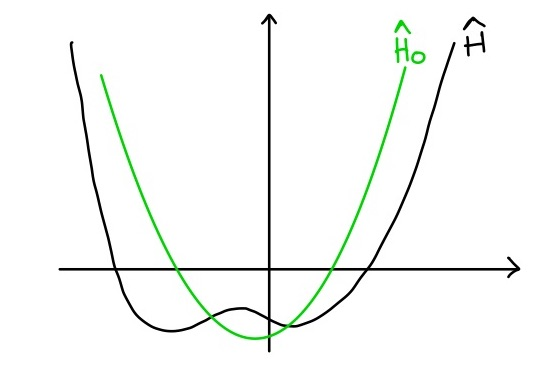
\includegraphics[scale=0.20]{img_1.jpg}
\caption{How to approximate an otherwise very difficult function with a known, simpler one.}
\label{fig:approximation}
\end{figure}
\textbf{1)} First we proceed by writing the S.E. with the truncated basis set.
\[
\hat{H}\bigg(\sum_{m=1}^{M}c_m^{(n)}\psi_m(x)\bigg)=E_n\bigg(\sum_{m=1}^{M}c_m^{(n)}\psi_m(x)\bigg)
\text{ where $c_m^{(n)}=\int dx\,\psi_m^*(x)\varphi_n(x)$}
\]
since the Hamiltonian operator is a function it can be propagated through the equation. Right now we are expanding $n$ and projecting it onto $m$.\\
\[
\sum_{m=1}^{M}c_m^{(n)}\,\hat{H}\psi_m=E_n\,\sum_{m=1}^{M}c_m^{(n)}\psi_m\]
\textbf{2)} We project both functions on the basis (scalar product). We multiply both sides for an arbitrary wave function $\psi_l$ (that we can supposedly solve).
\[\sum_{m=1}^{M}\,(\psi_l,\hat{H}\psi_m)c_m^{(n)}=E_n\,\sum_{m=1}^{M}c_m^{(n)}(\psi_l,\psi_m)
\]
The inner product between two functions gives an integer. \\
$H_{lm}=H_{ml}^*$ is an hermitian matrix that can be diagonalized to get the eigenvalues.\\
\[
\sum_{m}^{M}H_{lm}c_m^{(n)}=E^{(n)}c_l
\]
We reduced a complex problem to a conventional eigenvalue problem with a $H_{lm}$ matrix. The pain is to compute the $M$ integrals and to find an appropriate "problem B". As a results, this method is hardly applicable to any problems with more of 3 dimensions. \\

\section{Quantum tunneling - The Landau problem}
\begin{figure}[htbp!]
	\centering
	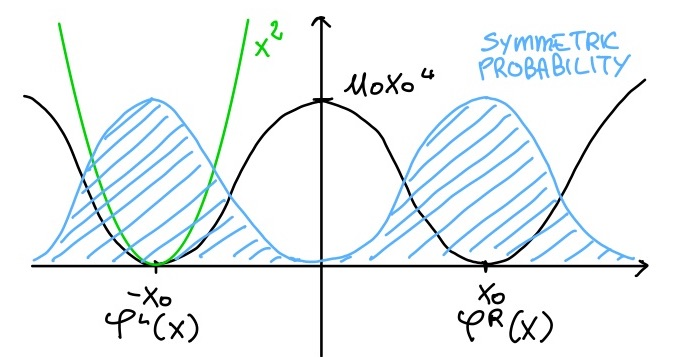
\includegraphics[scale=0.30]{img_2.jpg}
	\label{fig:ass}
	\caption{ass problem}
\end{figure}
The ass problem (because the potential kinda looks like an ass) is the gate to the understanding of quantum tunneling (necessary for quantum bonds, which are a reflection of the quantum tunneling behaviour). \\
The potential is: $U(x)=U_0(x^2-x_0^2)^2$.\\

The Hamiltonian for the wave function: $\hat{H}=-\frac{\hbar^2}{2m}\,\frac{d^2}{dx^2}+U_0\cdot(x^2-x_0^2)^2$
Note that this is a symmetric function, roughly composed by two gaussians, so we can approximate the function with an harmonic oscillator. Considering the potential to its lowest points it can be approximated and then expanded. \\

We have two basis elements, the two eigenstates $n=0,1$ (ground state and first excited state), and we whish to solve $hat{H}\varphi_n=E_n\varphi_n$, with $n=0,1$:

\[
\hat{H}\varphi_n=E_n\varphi_n
\begin{cases}
\varphi_0 \cong C_L^0\,\psi^L(x)+C_R^0\,\psi^R(x)\\
\varphi_1 \cong C_L^1\,\psi^L(x)+C_R^1\,\psi^R(x).
\end{cases}
\]
$C_L$ and $C_R$ are coefficients for each part of the function, one for each eigenstate. The values $\varphi_o$ adn $\varphi_1$ are the two eigenvalues of a $2 \times 2 $ matrix.\\
We then proceed to calculate the value of the matrices for the expansion.\\
\[
H_{RR}=(\psi_R,\hat{H}\,\psi_R)= \int\psi_R^*(x)\,\bigg[-\frac{\hbar^2}{2m}\,\frac{d^2}{dx^2}+U_0\cdot(x^2-x_0^2)^2\bigg]\,\psi_R(x)\,dx\]
\[
=\int\psi_R^*(x)\,\bigg[-\frac{\hbar^2}{2m}\,\frac{d^2}{dx^2}+\frac{1}{2}m\omega^2\cdot(x^2-x_0^2)^2\bigg]\,\psi_R(x)\,dx
\]
$U_0$ has been substitued with the potential energy of the harmonic oscillator approximation. The integral is computable with Taylor expansion because we consider the minimum of the function.
\[
U(x)=U(x_0)+U'(x_0)(x-x_0)+\frac{1}{2}\,U''(x_0)(x-x_0)+\dots\]
The final result is
\[
H_{RR}=\frac{1}{2}\hbar\omega
\]
and since this is a symmetrical problem we can also foresee that $H_{LL}\cong\frac{1}{2}\hbar\omega$.\\
The result of $H_{LR}=H_{RL}$ is expected to be very small because the probability of finding the particle in the middle of the harmonic oscillator is very small, i.e. when $\psi_L(x)$ is large, $\psi_R(x)$ is going o be small and viceversa.
\[
H_{RL}=H_{LR}=\int dx\,\psi_L(x)\hat{H}\psi_R(x) = \varepsilon
\]
Now we can calculate the matrix
\[
H_{mn}=
\begin{pmatrix}
E_0 & -\varepsilon\\
-\varepsilon & E_0
\end{pmatrix}
=
\begin{pmatrix}
\frac{1}{2}\hbar\omega & -\varepsilon\\
-\varepsilon & \frac{1}{2}\hbar\omega
\end{pmatrix}
=
E_0
\begin{pmatrix}
1 & -\frac{\varepsilon}{E_0}\\
-\frac{\varepsilon}{E_0} & 1
\end{pmatrix}
\]
\textbf{NB:} $E_0>>>\varepsilon$ because of the energy barrier due to $H_{mn}$.
\newline
We reduced a complex problem to a linear algebra problem: $\hat{H}\psi=E\psi \rightarrow H_{mn}C_n^{(l)}=E_lC_n^{(l)}$.\\
\newline
\textbf{Ansatz 1}: In the ground state I have 50\% probability of finding the particle
\[
\text{G.s.:}
\begin{pmatrix}
1 & -\frac{\varepsilon}{E_0}\\
-\frac{\varepsilon}{E_0} & 1
\end{pmatrix}
\begin{pmatrix}
1\\1
\end{pmatrix}
=
\frac{1}{\sqrt{2}}
\begin{pmatrix}
1-\frac{\varepsilon}{E_0}\\1-\frac{\varepsilon}{E_0}
\end{pmatrix}
\]
This ground state has slightly lower energy than the normal ground state
\[
\text{$1^{st}$ ex. st.:}
\begin{pmatrix}
1 & -\frac{\varepsilon}{E_0}\\
-\frac{\varepsilon}{E_0} & 1
\end{pmatrix}
\begin{pmatrix}
1\\-1
\end{pmatrix}
=
\biggl(1+\frac{\varepsilon}{E_0}\biggr)\cdot E_0 \cdot
\begin{pmatrix}
1\\-1
\end{pmatrix}
\]
\textbf{NB:} If the barrier is infinite the ground state is trivially degenerate. I then have two independent quantum systems. The particle cannot change its state. Instead, if the barrier is finite (slightly determined end of the barrier at very high energies) it splits into two states (\textbf{splitting states}) that interact with each other. The particle goes back to a 100\% probability of being in either one or another system. This is called \textbf{quantum superposition}.
\newline
Since the barrier is at very high energy, we could expect to find the correspondance principle at some point. Classical interpretation of the system at this point says that the particle could "decay" from a state of very high energy into one of the two ground states (50\% probability for each state, fair game). Quantum interpretation gives the 100\% probability to the electron of being in both the states at the same time.\\
\[
\begin{cases}
\varphi_0(x) = \frac{1}{\sqrt{2}}[\psi^L(x)+C_R^0\,\psi^R(x)]\\
\varphi_1(x) = \frac{1}{\sqrt{2}}[\psi^L(x)+C_R^0\,\psi^R(x)]
\end{cases}
\]
\newline
So, if at $t=0$, the  particle is on the left $\ket{\psi_0}=\ket{\psi_L}$, the function immediately after will be $\psi_L(x)$. However, if we wait long enough, the probability to find it in each state will be 50\% - 50\%. \\
What is the probability of finding the particle on the right at given time $t$? \\
$(P_R(t>0)=\,?$)\\
$P_L(t>0)=1-P_R(t>0)$\\
By definition $E_0=0, E_1= \varepsilon$. Consequently, $\varepsilon = E_1-E_0$\\
To find the probability of the particle being on the right/left, ($P_{R/L}(t)=|\braket{\psi_{R/L}\,|\,\varphi(t)}|^2$), we will use the time evolution operator.\\
\[
P_R(t)=|\braket{\psi_R\,|\,e^{-\frac{i}{\hbar}\cdot t \hat{H}}\,|\,\psi_L}|^2
\]
Minding that $\psi_R$ occurs at time $t$ whilst $\psi_L$ occurs at $t=0$.\\
If I want to check whether the particle is still on the left
\[
P_L(t)=|\braket{\psi_L\,|\,e^{-\frac{i}{\hbar}\cdot t \hat{H}}\,|\,\psi_L}|^2
\]
Let's first compute the probability for a small $t$. We perform the Taylor expansion of $e^{-\frac{i}{\hbar}\cdot t \hat{H}} = \mathds{1} -\frac{i}{\hbar}\cdot t\hat{H}$
\[
\ket{\psi_L}=\begin{pmatrix}
1\\0
\end{pmatrix}
\text{, }
\ket{\psi_R}=
\begin{pmatrix}
0\\1
\end{pmatrix}
\text{, }
\hat{H}=
\begin{pmatrix}
0 & \varepsilon\\ \varepsilon & 0
\end{pmatrix}
\]
\[
P_R(t)\cong\bigg|\braket{\psi_R\,|\,1-\frac{i}{\hbar}\cdot t \hat{H}\,|\,\psi_L}\bigg|^2 \cong
\bigg|(1,\,0) \cdot \mathds{1}
\begin{pmatrix}
0\\1
\end{pmatrix}
-\frac{i}{\hbar}\cdot t \cdot (1,\,0)
\begin{pmatrix}
0 & \varepsilon\\ \varepsilon & 0
\end{pmatrix}
(0,\,1)\bigg|^2
\]
\[
\cong \frac{t^2}{\hbar^2}\varepsilon
\]
but since $\frac{t\varepsilon}{\hbar}<<1$ we get $t << \frac{\hbar}{\varepsilon}$.\\
This is telling us that by waiting a little time the probability of finding the particle on the other side increases. This phenomenom is called \textbf{quantum tunneling}.\\
The conclusion up until this point is
\begin{itemize}
	\item A quantistic particle can cross an energy barrier, and the probability (or 		rate at which the transitions happen) is given by
	\[
	k=\frac{\varepsilon}{\hbar}
	\]
	which is an exponentially small amount.\\
	There is an analogy between thermal kinetic activation and quantum tunneling, both 	happen because of stochastic fluctuations. ($K\propto e^{\frac{\Delta V}{K_B T}}$)		. The difference is that in a quantum system this happens in quantum time and is 		not influenced by the temperature of the system.\\
	\item In quantum tunneling, the superposition between the higher energy levels 			that is caused by the lowering of the potential barrier causes the splitting of 		the lower energy levels. This is remarkably important when considering the 				\textbf{formation of the hydrogen bond $\rightarrow$ electron sharing is quantum 		tunneling!}\\
	At infinite distance we don't have any sharing because it's like having an 				infinite energy barrier. When the two atoms get close to each other, they share an 	electron via quantum tunneling, because of this then the energy levels split and 		create the two orbitals (bonding, antibonding).\\
\end{itemize}

For the final $t$ we cannot expand the exponent like we did before. Given $e^{-\frac{it}{\hbar}\hat{H}}\ket{\psi_R}$, we don't know $H\psi_R$, but can rewrite $\psi_R$ as linear combination of eigenstates of $H$:
\[
\text{ground state:} \ket{0}=\bigg(\frac{\ket{L}+\ket{R}}{\sqrt{2}}\bigg) \rightarrow \sqrt{2}\ket{0}= \ket{L}+\ket{R}
\]
\[
\text{first excited state:} \ket{1}=\bigg(\frac{\ket{L}-\ket{R}}{\sqrt{2}}\bigg) \rightarrow \sqrt{2}\ket{1}= \ket{L}-\ket{R}
\]
By summing and dividing,
\[
\begin{cases}
\ket{L}=\frac{1}{\sqrt{2}}\ket{\ket{0}+\ket{1}}\\
\ket{R}=\frac{1}{\sqrt{2}}\ket{\ket{0}-\ket{1}}
\end{cases}
\]
so we can substitute them:
\[
e^{-\frac{it}{\hbar}\hat{H}}\ket{R}=\frac{e^{-\frac{it}{\hbar}\hat{H}}}{\sqrt{2}}\cdot \ket{\ket{0}-\ket{1}}=\frac{1}{\sqrt{2}}\ket{0}-\frac{e^{-\frac{it}{\hbar}\varepsilon}}{\sqrt{2}}\ket{1}
\]
where $e^{-\frac{it}{\hbar}\varepsilon}$ is the relative weight of quantum superposition.\\
\newline
\[
P_L=|\braket{L\,|\,\psi(t)}|^2=\bigg|\bra {L}\bigg(\frac{1}{\sqrt{2}}\ket{0}-\frac{1}{\sqrt{2}}\cdot e^{-\frac{it}{\hbar}\varepsilon} \ket{1} \bigg)\bigg|^2
\]
Knowing that $\braket{L\,|\,L}=\frac{1}{\sqrt{2}}$ and $\braket{L\,|\,R}=0$,
\[
= \bigg|\frac{1}{2}\cdot \frac{1}{\sqrt{2}}\cdot e^{-\frac{it}{\hbar}\varepsilon} \cdot \braket{L\,|\,1}\bigg|^2=\bigg(\frac{1}{2}-\frac{1}{2}\cdot e^{-\frac{it}{\hbar}\varepsilon}\bigg)^2=\bigg[\frac{1}{2}-\frac{1}{2}\bigg(\cos\frac{\varepsilon t}{\hbar}+i\sin\frac{\varepsilon t}{\hbar}\bigg)\bigg]^2
\]
\[
P_L=\frac{1}{2}\bigg(1-\cos^2\frac{\varepsilon}{\hbar}t\bigg)
\]
For $t=0$, $P=0$ then $\cos^2x$ grows with a $t^2$ rate. There is an oscillation (figure \ref{fig:pulsation}) with a given period $T=\frac{\hbar}{2\varepsilon}$.\\
\begin{figure}[htbp!]
	\centering
	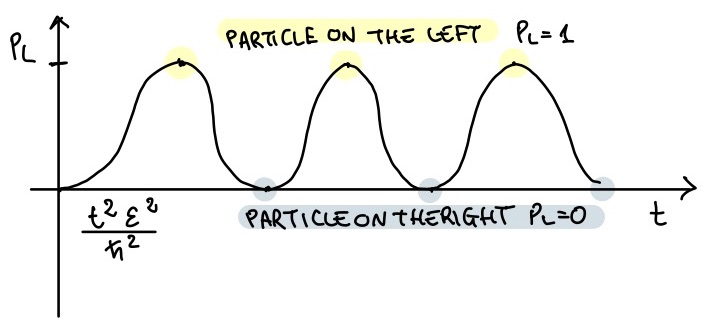
\includegraphics[scale=0.30]{img_3.jpg}

	\caption{The oscillatory behaviour here represented is called \textbf{quantum pulsation}.}
	\label{fig:pulsation}
\end{figure}
\newline

\section{Ritz-Rayleigh variational principle}
Suppose we want to estimate the ground state energy $E_0$ and corresponding wave function of the stationary Schr\"{o}dinger equation.\\
We define $\varphi(x)$ as a function approximating $\psi_0(x)$. Remember that it can always be written as:
\[
\varphi(x)=\sum_{n}^{\infty}c_n\psi_n(x),\;\;\; \hat{H}\psi_n=E_n\psi_n\, \text{ furthermore} \;\; \sum_{n=0}|c_n|^2=1
\]
We need to find any function approximating $\psi_0^{(x)}$, and we also assume that the wave function is already normalized. The expectation value for $\varphi$ is:
\[
\frac{\braket{\varphi\,|\,\hat{H}\,|\,\varphi}}{(\braket{\varphi \,|\, \varphi})}=
\sum_{n,m}c_n^{*}c_m\braket{\psi_n\,|\,\hat{H}\,|\,\psi_m}=\sum_{n,m}c_n^{*}c_mE_m\delta_{nm}=
\sum_{n}|c_n|^2E_n
\]
By assuming $c_n \geq 0$, the whole operation is $\geq E_0$ but this is true only if $\psi_n=\psi_0$.\\
\newline
TRIVIAL NOTE: if $\varphi(x)=\psi_0$ then we have a projection on a vector on itself:
\[
\begin{cases}
c_n=0, & n \neq 0\\
c_n=1, & n=0
\end{cases}
\]
\newline
The point here is that if we guess a function, compute the eigenvalues, and do the same with another function, the one that lowers the energy the most is the most accurate approximation of the wavefunction. E.g.:\\
Function 1 $\rightarrow$ Expected value $E_0$\\
Function 2 $\rightarrow$ Expected value $E_1$\\
$\rightarrow$ if $E_0 < E_1$ then $E_0$ is a better approximation of the wave function.\\
\newline
\noindent\rule{4cm}{0.1pt}
\newline
\textit{Example: Given $\varphi(x, \alpha)$, which is a family of wave functions, find $\psi_0(x)$ such as it is the best approximation of the family.} In other words, we need to evaluate the following equation\\
\[
\braket{\varphi_{\alpha}(x)\,|\,\hat{H}\,|\,\varphi_{\alpha}(x)}=E(\alpha)
\]
for whih $E$ is minimum. We must find the minimum of the function (derivative = 0).
\[
\frac{\partial}{\partial\alpha}E(\alpha)=0\, \text{  solve for  }\, \alpha=\alpha_{min}
\]
Find $\alpha$ such as $E_{\alpha min}$ is the best approximation of $E_0$ and $\varphi_{\alpha min}(x)$ is the best approximation of $\psi_0$. Putting it formally, if we have multiple parameters: $\varphi_{\alpha \dots \alpha_n(x)}$
\[
\braket{\varphi_{\alpha \dots \alpha_n(x)}\,|\,\hat{H}\,|\,\varphi_{\alpha \dots \alpha_n(x)}} = E_{\alpha \dots \alpha_n}
\]
We need to calculate the minimum of the multidimensional function:
\[
\nabla_{\alpha}E=0 \rightarrow
\begin{cases}
\frac{\partial}{\partial \alpha_1}=0 \rightarrow \alpha_1=\alpha_{1, min}\\
\dots\\
\frac{\partial}{\partial \alpha_n}=0 \rightarrow \alpha_n= \alpha_{n, min}\\
\end{cases}
\]
Doing so we find a collection of energies and wavefunctions. The more parameters we have, the more we can explore the space, but  we have no guarantee of finding the exact solution. Indeed, the probability of getting the right ground state is very low.
\newline
\noindent\rule{4cm}{0.1pt}
\newline
\\
So which are the steps of this approximation method? Let's go through them using the quantum harmonic oscillator.\\

Given the Hamiltonian equation for harmonic oscillator: $\hat{H}=-\frac{\hbar^2}{2m}\frac{d^2}{dx^2}+\frac{1}{2}m\omega^2x^2$\\
1) \textbf{Variational Ansatz}: We "guess" a normalized (the $4$ term is used for normalization) gaussian to best represent the harmonic oscillator: $\varphi_{\alpha}(x)=\bigg(\frac{1}{\sqrt{2\pi}\alpha}\bigg)^{1/2}e^{-{\frac{x^2}{4\alpha^2}}}$\\

2) \textbf{Computation of $E(\alpha)$} by first evaluating the hamiltonian function of $\varphi_{\alpha}(x)$ (first fragment, so to say)
\[
-\frac{\hbar^2}{2m}\frac{d^2}{dx^2}\varphi_{\alpha}(x)=\]
\[=\,-\frac{\hbar^2}{2m}\bigg(\frac{1}{\sqrt{2\pi}\alpha}\bigg)^{1/2}\frac{d}{dx}e^{-{\frac{x^2}{4\alpha^2}}}\]
\[
=\,\frac{\hbar^2}{2m}\bigg(\frac{1}{\sqrt{2\pi}\alpha}\bigg)^{1/2}\cdot\frac{2x}{4\alpha^2}e^{-{\frac{x^2}{4\alpha^2}}}
\]
\[
=\,\frac{\hbar^2}{2m}\bigg(\frac{1}{\sqrt{2\pi}\alpha}\bigg)^{1/2}\cdot\frac{d}{dx}\frac{x}{2\alpha^2}e^{-{\frac{x^2}{4\alpha^2}}}
\]
\[
=\,\frac{\hbar^2}{2m}\bigg(\frac{1}{\sqrt{2\pi}\alpha}\bigg)^{1/2}\cdot\bigg(\frac{1}{2\alpha^2}e^{-{\frac{x^2}{4\alpha^2}}}-\frac{x^2}{2\alpha^2}e^{-\frac{x^2}{4\alpha^2}}\bigg)
\]
\[
=\,\frac{\hbar^2}{2m}\bigg(\frac{1}{\sqrt{2\pi}\alpha}\bigg)^{1/2}\cdot\frac{1}{2\alpha^2}\cdot\bigg(1-\frac{x}{2\alpha^2}\bigg)e^{-{\frac{x^2}{4\alpha^2}}}
\]
Which ultimately results in (also quantum oscillation period?):
\[
T=\frac{\hbar^2}{4m\alpha^2}\bigg[1+\frac{x^2}{2\alpha^2}\bigg]e^{-{\frac{x^2}{4\alpha^2}}}\cdot\frac{1}{(\sqrt{2\pi}\alpha)^{1/2}}
\]
And go on with the evaluation of $E(\alpha)$.
\[
E(\alpha)=\frac{1}{\sqrt{2\pi}\alpha}\cdot \int dx\, e^{\frac{x^2}{2\alpha^2}}\bigg[\frac{\hbar^2}{4m\alpha}\bigg(1+\frac{x^2}{2\alpha^2}\bigg)+\frac{1}{2}m\omega^2x^2\bigg]=
\]
\[
=\frac{1}{\sqrt{2\pi}\alpha}+\bigg(\frac{\hbar^2}{8m\alpha^4}+\frac{1}{2}m\omega^2\bigg)\cdot \int\,dx\,\frac{e^{\frac{x^2}{2\alpha^2}}}{\sqrt{2\pi}\alpha}x^2
\]
The integrand is called \textbf{gaussian variance} and it is equal to $\mathbf{\alpha^2}$. So
\[
E(\alpha)=\bigg(\frac{1}{4}+\frac{1}{8}\bigg)\frac{\hbar^2}{m\alpha^2}+\frac{\alpha^2}{2}m\omega^2 = \frac{3}{8}\frac{\hbar^2}{m\alpha^2}+\frac{\alpha^2}{2}m\omega^2
\]
The latter sum is a sum of two energy values.
\begin{figure}[htbp!]
	\centering
	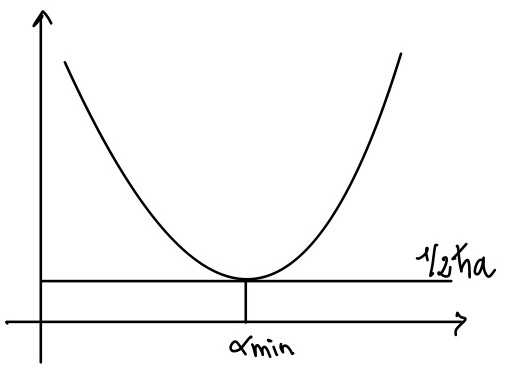
\includegraphics[scale=0.20]{img_4.jpg}
	\caption{In this picture we can see a point of intersection becuase we get the exat result.}
	\label{fig:intersect}
\end{figure}
To find $\alpha_{min}\rightarrow\frac{\partial}{\partial \alpha}E(\alpha)=0$
\[
\frac{\partial}{\partial \alpha}E(\alpha)=-2\cdot\frac{3}{8}\frac{\hbar}{m\alpha^{3}}+\alpha m\omega^2=0
\]
Multiply by $\alpha^3$ both sides:
\[
\frac{\partial}{\partial \alpha}E(\alpha)=-\frac{\hbar}{m}+\alpha^4m\omega^2=0
\]
%notare che il prof aveva sbagliato a mettere il fattore della gaussiana
\[
\alpha^2=\sqrt{\frac{\hbar^2}{m^2\omega^2}}
\]
This is the same result we got for the quantum harmoni oscillation problem! Keep in mind that this method \underline{only} applies to the ground state.

    \graphicspath{{chapters/06/}}
\chapter{Atomic physics}
\section{Quantum theory of the Hydrogen atom}
\subsection{Evaluation of conservation of energy}
Remember that when talink about classical theory of the hydrogen atom we simplified the problem by switching from Cartesian to polar coordinates and, by applying the conservation laws, we obtained:
\[
E=\frac{1}{2}m\bigg(\frac{d}{dt}n\bigg)^2+\frac{L^2}{2mr^2}+U(r)
\]
that can be represented in quantum mechanics with the hamiltonian. The hamiltonian in polar coordinates is written as
\[
\hat{H}=(-\frac{\hbar^2}{2m^2}\, \nabla - \frac{e^2}{r})
\]
The best evaluation of the hamiltonian for the quantum analysis of the hydrogen atom is obtained by using the \textbf{spherical coordinates}. Nabla (the Laplacian) in spherical coordinates $(r,\theta,\varphi)$ is hence written as:
\[
\nabla^2=\frac{1}{r^2}\frac{\partial^2}{\partial r^2}+\frac{1}{r^2}\cdot\bigg(\frac{\partial^2}{\partial \theta^2}+\frac{1}{\tan\theta}\frac{\partial}{\partial\theta}+\frac{1}{\sin\theta}\frac{\partial^2}{\partial\varphi^2}\bigg)
\]
The hamiltonian so becomes:
\[
\hat{H}=\frac{\hbar^2}{2mr^2}\frac{\partial^2}{\partial r^2}+\frac{\hbar^2}{2mr^2}\cdot\bigg(\frac{\partial^2}{\partial \theta^2}+\frac{1}{\tan\theta}\frac{\partial}{\partial\theta}+\frac{1}{\sin\theta}\frac{\partial^2}{\partial\varphi^2}\bigg)-\frac{e^2}{r}
\]
The first part is called \textbf{radial part} because it's $r$-dependent only, the other is the \textbf{angular part}.\\
Now we can consider the angular momentum in classical mechanics and quantum mechanics:
\[
\vec{L}=\vec{r}\times\vec{p}=\vec{r}\times(-i\vec{\nabla}\hbar)
\]
\[
\textit{Fact} \rightarrow \vec{\hat{L^2}}=\hat{L_x}\hat{L_x}+\hat{L_y}\hat{L_y}+\hat{L_z}\hat{L_z}
\]
This is corresponding to the angular part of the hamiltonian that can be rewritten in sperical coordinates with the inclusion of the angular momentum multiplied by $\hbar^2$.
\[
\hat{H}=\frac{\hbar^2}{2mr^2}\frac{\partial^2}{\partial r^2}+\frac{\hat{L^2}}{2mr^2}-\frac{e^2}{r}
\]
The fact that the angular momentum is not present in the radial part of the hamiltonian means that the two operators must commute $[\hat{H},\,\hat{L^2}]=0$ and they must also share the same eigenstates. It's also important to note that the invidual components of the angular momentum only commute with $\hat{L^2}$ but not with each other.\\
\[
\begin{cases}
[\hat{L_i},\,\hat{L_j}]\neq0 & i,j=1, 2, 3, ...\\
[\hat{L_i},\,\hat{L^2}]=0
\end{cases}
\]
\\
These are called \textbf{spherical harmonics}, they depend on two quantum numbers because they use two different operators and are only part of the angular part of the hamiltonian.\\
\[
\begin{cases}
\hat{L_z}Y_{lm}(\theta,\varphi)=\hbar mY_{l,m}(\theta,\varphi) & m = l, -l+1,..., 0,..., -l \,\text{(projection)}\\
\hat{L^2}Y_{lm}(\theta,\varphi)=\hbar^2 l(l+1)Y_{l,m}(\theta,\varphi) & l = 0, 1, 2, ... \,\text{(max length,)}\, m < l^2
\end{cases}
\]
\textbf{N.B.:} in this way we obtain the quantization of $\hat{L_j}$ and $\hat{L^2}$.\\
Where $m$ represents the projection (bounded to $l$), and $l$ the length. Note that we wrote $l(l+1)$ and not $l^2$, the difference only matters in the quantum realm and it is noticeable when $l$ is small. For larger $l$ we go back to the classical realm (correspondence principle).\\
The wave function can then undergo variables separation, this implies the fact that eigenstates of the hamiltonian are also eigenstates of the square of the angular momentum.
\[
\Psi_{n,l,m}(r,\theta,\varphi)=R(r)\cdot Y_{l,m}(\theta,\varphi)
\]
I can calculate the hamiltonian of the newly obtained wave function.
\[
\hat{H}\psi_{n,l,m}=\bigg[\frac{-\hbar^2}{2mr^2}\frac{\partial^2r}{\partial r^2}R_nY_{l,m}+\frac{\hbar^2l(l+1)}{2mr^2}R_nY_{l,m}-\frac{e^2}{r}R_nY_{l,m}\bigg]=E_{n,m,l}R_nY_{l,m}
\]
By eliminating $Y_{l,m}$ we obtain the \textbf{one-dimensional Schr\"odinger equation}, I obtain one equation for each value of $l$. Each equation is referred to a different expression of energy.
\[
\frac{-\hbar^2}{2mr^2}\frac{\partial^2r}{\partial r^2}R_n+\frac{\hbar^2l(l+1)}{2mr^2}R_n-\frac{e^2}{r}R_n=E_{n,m,l}R_n
\]
\\

\subsection{Angular momentum conservation}
We can also rewrite kinetic energy in a polar form.\\
\[
-\frac{\hbar^2}{2m}\nabla^2 \rightarrow-\frac{\hbar^2}{2m}\frac{1}{r}\frac{\partial^2}{\partial r^2}\dot{r}+\frac{\hat{L^2}}{2mr^2} = \hat{T_r}+\hat{T}_{(\theta,\varphi)}
\]
Where $\hat{T_r}$ is the radial component of kinetic energy, $\hat{T}_{(\theta,\varphi)}$ is the angular component of kinetic energy. Note that if the radial part is applied to a radial function $rR(r)$, the second derivative applies to the product of $r$ and the function, not just to $r$.
\[
R(r)=\frac{1}{r}\frac{\partial^2(r\cdot R(r))}{\partial r^2}
\]
As we said before, the hamiltonian commutes with the square of the angular momentum $[\hat{H},\,\hat{L^2}]=0$ because the angular momentum doesn't have any derivatives with respect to $r$. By considering the hamiltonian as $\hat{H}=\hat{T_r}+\hat{V}$ with $\hat{V}$ as describing the coulomb potential, these commutations are possible:\\
\[
[\hat{T_r}\,,\,\hat{L^2}]=0\,,\,\,\,[\hat{V}\,,\,\hat{L}]=0\,,\,\,\,[\hat{L^2}\,,\,\hat{L^2}]=0
\]
All these have common sets of eigenstates. Note that $\hat{T_r}\,,\,\hat{L^2}]=0$ is possible beacuse $\hat{T_r}$ doesn't depened on $\theta$ \\
\newline
We can implement the fact that the operators, as said above, share a common set of eigenstate by pluggin the following:
\[
\psi_{nml}(r, \theta, \varphi) = R_n(r)Y_{lm}(\theta, \varphi)
\]
in the Schr\"odinger equation, obtaining a family of equations, one for each unit of angular momentum:
\[
\frac{-\hbar^2}{2mr^2}\frac{\partial^2r}{\partial r^2}R_n+\frac{\hbar^2l(l+1)}{2mr^2}R_n-\frac{e^2}{r}R_n=E_{n,m,l}R_n
\]
$l=0 \rightarrow$ \textbf{s-state}: $\frac{-\hbar^2}{2mr^2}\frac{\partial^2r}{\partial r^2}R_n-\frac{e^2}{r}R_n=E_{n,l}R_n$\\
\\
$l=1 \rightarrow$ \textbf{p-state}: $\frac{-\hbar^2}{2mr^2}\frac{\partial^2r}{\partial r^2}R_n+\frac{3\hbar^2}{2mr^2}R_n-\frac{e^2}{r}R_n=E_{n,m,l}R_n$\\
\\
$l=2 \rightarrow$ \textbf{d-state}: $\frac{-\hbar^2}{2mr^2}\frac{\partial^2r}{\partial r^2}R_n+\frac{6\hbar^2}{2mr^2}R_n-\frac{e^2}{r}R_n=E_{n,m,l}R_n$\\
\\
We can infer from these equation that we get stronger repulsions between states as $l$ grows (graphs of such functions shown in figure \ref{fig_swaves}).\\
\begin{figure}[htbp!]
	\centering
	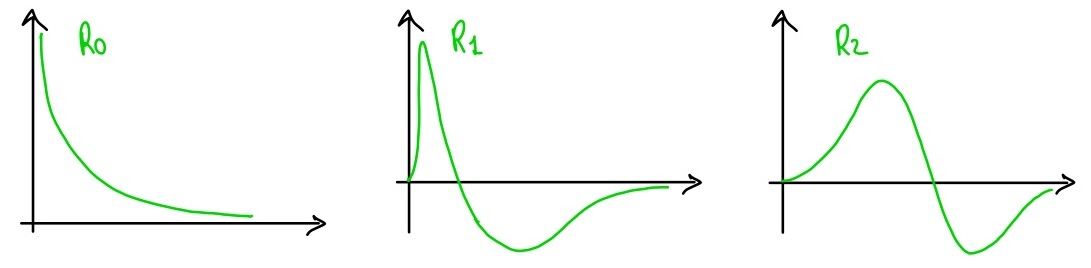
\includegraphics[scale=0.30]{img_5}
	\caption{Representation of s-waves}
	\label{fig_swaves}
\end{figure}
\textbf{N.B.}: defining $U(r) \equiv rR(r)$ implies
\[
-\frac{\hbar}{2m} \frac{d^2}{dr^2} U(r) + \frac{\hbar l(l+1)}{2mr^2} U(r) - \frac{e^2}{r} u(r) = E U(r)
\]
Where $u(r)$ is not a potential. When we tried to solve the h-atom with classical mechanics, the analogy with the kinetic energy was perfect. This is not quite the case?
Finally we want to calculate the probability of a particle to be at distance $r$.
\[
drProb(r)=|R(r)|^2r^2dr
\]
\[
P(\vec{r},\vec{r}+dr)=\int_{\vec{r}}^{\vec{r}+dr}dr\,r^2\iint d\theta\,d\varphi\,|R(r)\,Y(\theta,\varphi)|^2=\int_{\vec{r}}^{\vec{r}+dr}dr\,r^2R^2(r)\iint_{sph}\,d\theta\,d\varphi|Y|^2
\]
Since the function is not dependent on $\theta$ or $\varphi$, the integral equals 1.
\[
P(\vec{r},\vec{r}+dr)=\vec{r}^2R^2(r)dr
\]
Depending on the value of $l$ I can get the probability of the electron depending on $\theta$ and $\varphi$. At $l=0$ the probability is more concentrated on the centre and then fades out (s orbital). At $l=1$ the function depends on $\theta$ but not on $\varphi$, the function is cylindrically symmetrical (p orbital). It is important to remember that there is no orbit in an atom, for the concept of trajectory breaks down on a quantum level.\\
\\

\section{Relationship between spin and statistics: Quantum many-body systems}
\subsection{The importance of spin}
Spin statistics can explain chemistry, quantum entanglement, and quantum computers.\\
Stern Gerlach experiments confirm the fact that electrons have a magnetic moment, which is quantised in integers or half integers, because they can interact with a magnetic field. Generally, particles behave differently and may have different states of being.\\
What we know is that we cannot measure more than one component of the magnetic moment (quantum uncertainty) and this \textbf{intrinsic} magnetic moment behaves like an angular momentum.\\
The rotation of the electron upon itself generates a magnetic field and a magnetic moment. This is called \textbf{spin}, $\hat{S^2},\hat{S_z}$ a property of particles that \textbf{doesn't change with time} and that can distinguish a particle from one another.\\
\newline
We assume that:
\[ [\hat{S_x}\,,\,\hat{S_y}]=i\hbar\hat{S_z} \]
\[ [\hat{S_z}\,,\,\hat{S^2}]=\hat{0} \]
The values of $\hat{S^2}$ characterize the behaviour of the particle.\\
\[\hat{L^2}\,\rightarrow\,l=0, 1, 2, ...\]
\[\hat{S^2}\,\rightarrow\,s=0, \frac{1}{2}, 1, \frac{3}{2}, ...\]
Electrons, neutrons, and protons have $s=1/2$. Photons, for instance, have $s=1$.\\

\subsection{Spin-Statistics theorem (in identical particles}
Let's consider a wave function of many identical particles $\psi$, for instance $n$ identical electrons with spin $s$, $\hat{S_z}$, and position $r$. All the particles have the same velocity.\\
\[
\Psi(\vec{r_1}, s_1^z, \vec{r_2}, s_2^z, ..., \vec{r_n}, s_n^z) \text{   ,with } \vec{q}=(\vec{r},\vec{s_z})
\]
\[\Psi(\vec{q_1},\vec{q_2}, ..., \vec{q_n}) \]
\textbf{antisymmetric wave-function (fermions)}: wave-function that under the exchange of pairs of identical particles has a total spin, $s$, that is an \textbf{half integer} (1/2, 3/2, ...). Swapping the wave function \textbf{changes} it.\\
\[\Psi(\vec{q_1},\vec{q_2}, ..., \vec{q_n})=-\Psi(\vec{q_1},\vec{q_2}, ..., \vec{q_n})\]
The particles that have an antisymmetric wavefunction are called \textbf{fermions}.\\
\newline
\textbf{symmetric wave-function (bosons)}: wave function that under the exchange of pairs of identical particles has a total spin, $s$, that is an \textbf{integer} (1, 2, 3, ...). Swapping the wave function \textbf{doesn't change} it.\\
\[\Psi(\vec{q_1},\vec{q_2}, ..., \vec{q_n})=\Psi(\vec{q_1},\vec{q_2}, ..., \vec{q_n})\]
The particles that have an antisymmetric wavefunction are called \textbf{bosons}.
\begin{quote}
"A fermion once, a fermion forever".
"fermions and bosons are like Montecchi and Capuleti. They don't want anyhing to do with each other"
- Pietro Faccioli
\end{quote}
\noindent
\textbf{Corollary}: In a quantum wave function, there cannot be two fermions with identical state or else two identical fermions cannot be found in the same quantum state.
\[\Psi(q_1, q_2)= -\Psi(q_2,q_1)\] the two electrons are the same, $q_1=q_2=q$
\[\Psi(q,q)=-\Psi(q,q) \]
The only condition for which this equality is true is for  $\Psi = 0$. This is called \textbf{Pauli's exclusion principle}.
\\
\subsection{Mean Field Approximation}
Solving the S.E. for more than one particle rapidly becomes challenghing, even resorting to High Performance Computing. However, much of the global, qualitative structure of the Mondelyev table can be understood within a simple \textbf{mean field} picture: instead of accounting for all pairwise Coulomb interactinos, we assume that the effect on each electron, due to all other electrons and the protons can be represented by an overall confining potential.\\
Suppose we are dealing with two electrons:
\[
\bigg(-\frac{\hbar^2}{2m}\sum_{i}^{N}\nabla^2_i+U(\vec{r_1}...\vec{r_n})\bigg)\Psi(\varphi_1 ... \varphi_n)=E\Psi(q_1 ... q_n)
\]
The solution to the eigenvalue problem that is also antisymmetric to the potential depends on the position.
\[
U(\vec{r_1}...\vec{r_n})=\sum_{i,j}\frac{e^2}{|\vec{r_i}-\vec{r_j}|}-e^2\frac{\mathbb{Z}}{r_i}
\]
Instead of keeping track of all the interactions of particles on one another, we consider the average of the whole many-body system, e.g., mean coulombic repulsion. I calculate the interaction between single electron and average electron density. The larger symmetry is the ground state, which for the H-atom this is \textbf{1s}, as shown in figure \ref{fig:spin1}.\\
\begin{figure}[htbp!]
	\centering
	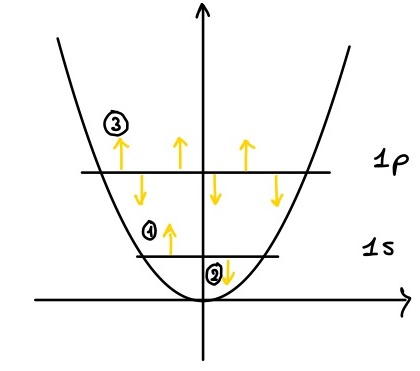
\includegraphics[scale=0.20]{img_6}
	\caption{Position of electrons in the 1p and 1s states with relative spin (up pr down)}
	\label{fig:spin1}
\end{figure}
\\
The structure of the wave function is influenced by spin even if it doesn't appear in the hamiltonian and can be used not only for electrons but for all subatomic/subnuclear particles. \\
We may ask ourselves: is there any stable nucleus? For clarity, a nucleus is divided into two different type of nucleons, protons and neutrons. Nucleons can have two different states: spin up (protons) and spin down (neutrons). Actually, the spin is really the only thing that allow us to differentiate the two, since their mass is basically the same (neutrons have a little heavier mass). For each spin there's an isospin up and an isospin down (isospin measures the charge). An example of (impossible) nucleus decay is shown in figure \ref{fig:decay}.\\
\begin{figure}[htbp!]
	\centering
	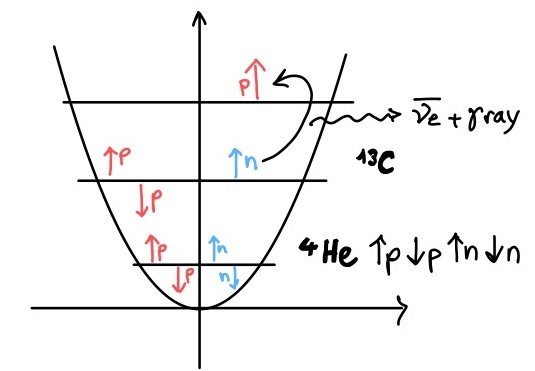
\includegraphics[scale=0.20]{img_7}
	\caption{In this picture the $He^4$ nucleus is represented. It it the most stable nucleus ($\alpha$particle). The thing is that the difference in mass ($m_n > m_p$) $\Delta m \rightarrow \text{energy}$ is not sufficient to reach the higher energy state and become a proton. Is there any other way? No, because of the spin theory. So, even if in principle a neutron could decay into a proton, ultimately Pauli's exclusion principle does not allow to have the same spin.}
	\label{fig:decay}
\end{figure}\\


\subsection{Quantum Entanglement}
In an external/mean potential, the Schr\"odinger equation has a potential of a single coordinate that depends on where that potential is located, thanks to the mean field approximation.
\[
\hat{H}=-\frac{\hbar^2}{2m}\sum_{i}\nabla_i^2+\sum_{i=1}^NU(q_i)=\sum_i h_i
\]
When $\hat{H}$ is separable into two parts, the wave function is the product of these two parts.\\
Consider N identical spin-0 bosons (simplest system that represents the sum of all possible permutations for N > 2):\\
\[
\Psi(r_1, ..., r_n)= \prod_K^n\varphi_n(r_i)=\varphi_1(r_1)\cdot ... \cdot \varphi_n(r_n)
\]
If I swap two excited states eg., $\varphi_s(r_3)$ and $\varphi_p(r_1)$, I do not obtain the same wave function (I get $\varphi_s(r_1)$ and $\varphi_p(r_3)$) so they are antisymmetric. If I swap two ground states they stay the same (they are symmetric). This system is also used for distinguishable particles (boltzmanions) or identical particles in semiclassic regimes.\\
\newline
Consider now two identical fermions described by single-electron wave functions.\\
\[
\Psi(r_1, s_1^2, r_2, s_2^2)=\varphi_{\uparrow}(r_1)\varphi_{\downarrow}(r_2)
\]
We can prove that the wave function of the two different fermions (hence each one is described by a different spin state) system is antisymmetric. This is called \textbf{Slater determinant} for N>2 fermions.
\[
\Psi=\frac{1}{\sqrt{2}}\big(\varphi_{\uparrow}(r_1)\varphi_{\downarrow}(r_2)+\varphi_{\uparrow}(r_2)\varphi_{\downarrow}(r_1)\big)
\]
by swapping their indices
\[
\Psi'=\frac{1}{\sqrt{2}}\big(\varphi_{\uparrow}(r_2)\varphi_{\downarrow}(r_1)-\varphi_{\uparrow}(r_1)\varphi_{\downarrow}(r_2)\big)
\]
and it's noticeable how $\Psi = -\Psi'$. The two functions are antisymmetric.\\
This represents a quantum superposition of states. In order to follow Pauli's principle, each state has a 50\% of probability to occur and when $r_1$ is $\uparrow$,  $r_2$ must necessarily be $\downarrow$. We found out that Pauli's principle \textbf{entangles}particles. In our case with two fermions, the state of particle n.2 is entangled to the state of particle 1.

\begin{center}
\textbf{Quantum entanglement}: a physical phenomenon that occurs when a group of particles are generated, interact, or share spatial proximity in a way such that the quantum state of each particle of the group cannot be described independently of the state of the others, including when the particles are separated by a large distance.
\end{center}

The two particles are said to be an \textbf{EPR pair} (Einstein-Podolsky-Rosen) and the state of the two particles is called a \textbf{Bell state}.
If I measure spin 1, the wave function collapses into spin value 1 and spin 2 consequently collapses into spin value 2.\\
The concept of \textbf{quantum entanglement} has no correspondences in classical mechanics and is used to develop quantum computers.\\
In classical computers the iformation is carried on in one single state out of two (either the gate is open or is closed, binary system). In quantum computers I have N states, I have $2^N$ states entangled with each other at the same time. I can store much more information in $2^N$ compared to 1 \footnote{It may confuse a little, beacause we know that in a classical architecture, N bits can represent $2^N$ numbers. This formulation is not very correct and I will provide my own understanding on the matter. That is, with N bits we can ultimately have just one number, even if we have N possible ways to arrange the bits. Instead, a quantum architecture supports $2^N$ states \textit{simultaneously}. This more expressive power contributes to the idea of "quantum supremacy".}. \\
\newline
The antisymmetric equation is the determinant of this matrix:
\[
\frac{1}{\sqrt{2}}
\begin{pmatrix}
\varphi_1(r_1)&\varphi_2(r_1)\\
\varphi_1(r_2)&\varphi_2(r_2)
\end{pmatrix}
\]
that can be generalized into
\[
\frac{1}{\sqrt{2}}
\begin{pmatrix}
\varphi_1(r_1)&...&\varphi_n(r_1)\\
... & &...\\
\varphi_1(r_m)&...&\varphi_n(r_m)
\end{pmatrix}
\]
This latter matrix is called \textbf{Slater matrix} and I can calculate Slater determinant that guarantees that the wave function is antisymmetric.\\
\newline
The spin $\hat{S^2}$ doesn't have a classical correspondence, we cannot directly obtain a formula for $\hat{S^2}$ in classical mechanics. I must find objects that have two states.\\
Consider spin $1/2$ only and choose an Hillbert space and an operator that acts on it. Since a particle with $s=1/2$ can have two different states, the most natural choice for a Hillbert space would be \emph{$L^2$}.\\
The eigenstates of the z-components are:
\[\ket{\uparrow}=\begin{pmatrix}1\\0\end{pmatrix}\, \ket{\downarrow}=\begin{pmatrix}0\\1\end{pmatrix}\]
$\hat{S_x}$, $\hat{S_y}$, and $\hat{S_z}$ are represented by 2x2 matrices that must obey the commutation rule of $[\hat{S^2}\,,\,\hat{S_z}]=0$ and $[\hat{S_x}\,,\,\hat{S_y}]=i\hbar\hat{S_z}$.
\\
\textbf{Pauli matrices:}
\[
\hat{S_x}=\frac{\hbar}{2}\begin{pmatrix}0&1\\1&0\end{pmatrix}\;\,
\hat{S_y}=\frac{\hbar}{2}\begin{pmatrix}0&-i\\i&0\end{pmatrix}\;\,
\hat{S_z}=\frac{\hbar}{2}\begin{pmatrix}1&0\\0&-1\end{pmatrix}
\]
The normalized eigenstates for the x-component are:
\[
\ket{\rightarrow}=\frac{1}{\sqrt{2}}\begin{pmatrix}1\\1\end{pmatrix}\;\,
\ket{\leftarrow}=\frac{1}{\sqrt{2}}\begin{pmatrix}1\\-1\end{pmatrix}\,
\]
We can find the conditional probability of finding spin up with the condition of being in a state of spin left (but also spin up given spin up, etc.).
\[
P(\ket{\uparrow}|\ket{\leftarrow})=\bigg(\frac{1}{\sqrt{2}}\begin{pmatrix}1&0\end{pmatrix}\begin{pmatrix}1\\-1\end{pmatrix}\bigg)^2=\frac{1}{2}
\]
\[
P(\ket{\uparrow}|\ket{\uparrow})=\bigg(\frac{1}{\sqrt{2}}\begin{pmatrix}1&0\end{pmatrix}\begin{pmatrix}1\\0\end{pmatrix}\bigg)^2=1
\]
\[
P(\ket{\leftarrow}|\ket{\uparrow})=\bigg(\frac{1}{\sqrt{2}}\begin{pmatrix}1&-1\end{pmatrix}\begin{pmatrix}1\\0\end{pmatrix}\bigg)^2=\frac{1}{2}
\]
This is also the mathematical formalism that represents the Stern Gerlach experiment. In fact, if we calculate $P(\ket{\uparrow}|\ket{\leftarrow}) = \frac{1}{2}$, then $P(\ket{\uparrow}|\ket{\uparrow}) = 1$, we will get again $P(\ket{\uparrow}|\ket{\leftarrow}) = \frac{1}{2}$.  \\
We can calculate $\hat{S^2} = \hat{S_x}^2+\hat{S_y}^2+\hat{S_z}^2$ that results in a sum of identity matrices, in fact
\[\hat{S^2}=\frac{3}{4}\hbar^2\big(\mathds{1}_e\big)\]
The identity matrix $\\mathds{1}_e$ allows $\hat{S^2}$ to commute with every component of the spin operator.

\subsection{Tensor product states}
Up until now, we learned how to deal with spin's degrees of freedom only. But how do we integrate spin in the $L_2$ space of the wave function? We'll use the tensor product. Given two vectors, the definition of tensor product is:
\[
\begin{pmatrix}a_1\\a_2\\...\\a_n\end{pmatrix}\otimes\begin{pmatrix}b_1\\b_2\\...\\b_n\end{pmatrix}=\begin{pmatrix}a_1b_1\\a_1b_2\\...\\a_1b_n\\a_2b_1\\a_2b_2\\...\\a_mb_n\end{pmatrix}
\]
Tensor product is obtained by multiplying each $a$ term with every $b$ term. It creates another vector space (a larger Hillbert space) that is used to combine spins for many particles, spin and particle space of one particle ect.\\
Tensor product is used to describe the \emph{combination of two quantum states}.
\[\text{Quantum state of particle 1: } \begin{pmatrix}\alpha_1\\\alpha_2\end{pmatrix}=\alpha_1\begin{pmatrix}1\\0\end{pmatrix}+\alpha_2\begin{pmatrix}0\\1\end{pmatrix}=\alpha_1\ket{\uparrow}+\alpha_2\ket{\downarrow}=\vec{\ket\alpha}\]
\[\text{Quantum state of particle 2: } \begin{pmatrix}\beta_1\\\beta_2\end{pmatrix}=\beta_1\begin{pmatrix}1\\0\end{pmatrix}+\beta_2\begin{pmatrix}0\\1\end{pmatrix}=\beta_1\ket{\uparrow}+\beta_2\ket{\downarrow}=\vec{\ket{\beta}}\]
\marginpar{\textit{These single quantum states represent qubits}}
\[\text{Combination of the two states: }
\vec{\ket{\alpha}}\otimes\vec{\ket{\beta}}\equiv{\ket{\vec{\alpha}\vec{\beta}}}=\begin{pmatrix}\alpha_1\beta_1\\\alpha_1\beta_2\\\alpha_2\beta_1\\\alpha_2\beta_2\end{pmatrix}
\]
The combination of the two states creates a wavefunction which amplitude corresponds to the observation of all the combinations of the particles. For example, $\alpha_1\,\beta_1$ is the amplitude of observing the first particle $\uparrow$ and the second particle $\uparrow$ \\
We can build the basis for a vector product of two particles and with this we can describe four different states since $\mathbb{R}^2\otimes\mathbb{R}^2=\mathbb{R}^4$
\[
\begin{pmatrix}1\\0\\0\\0\end{pmatrix}=\ket{\uparrow\uparrow}\begin{matrix}\alpha_1=1\\\beta_1=1\end{matrix}\bigg| \;\;
\begin{pmatrix}0\\1\\0\\0\end{pmatrix}=\ket{\uparrow\downarrow}\begin{matrix}\alpha_1=1\\\beta_2=1\end{matrix}\bigg| \;\;
\begin{pmatrix}0\\0\\1\\0\end{pmatrix}=\ket{\downarrow\uparrow}\begin{matrix}\alpha_2=1\\\beta_1=1\end{matrix}\bigg| \;\;
\begin{pmatrix}0\\0\\0\\1\end{pmatrix}=\ket{\downarrow\downarrow}\begin{matrix}\alpha_2=1\\\beta_2=1\end{matrix}\bigg|
\]
We can also derive the most general quantum mechanical state description of the EPR pair:
\[
\ket{\vec{\alpha}\vec{\beta}}=\alpha_1\beta_1\ket{\uparrow\uparrow}+\alpha_1\beta_2\ket{\uparrow\downarrow}+\alpha_2\beta_1\ket{\downarrow\uparrow}+\alpha_2\beta_2\ket{\downarrow\downarrow}
\]
In this way I can carry on information about multiple state simultaneously.\\
\newline
Given $\varphi(x)$ wavefunction lives in a \emph{$L^2$} Hillbert space.\\
\[
\varphi(x)\otimes(\alpha\ket{\uparrow}+\beta\ket{\downarrow})=\begin{pmatrix}\alpha\varphi(x)\\\beta\varphi(x)\end{pmatrix}=\begin{pmatrix}\varphi_{\uparrow}(x)\\\varphi_{\downarrow}(x)\end{pmatrix}
\]
This latter matrix is called a \textbf{spinor}, which is a wavefunction that includes spin amplitude (usually wavefunction doesn't have information about spin of the particle).\\
Let's consider a \underline{non-entangled state}.
\[
\ket{\Psi}=\frac{1}{\sqrt{2}}\ket{\uparrow\uparrow}+\frac{1}{\sqrt{2}}\ket{\uparrow\downarrow}=\ket{\alpha\uparrow}
\]
The two measures are independent of each other, I can find particle 2 with a probability which is independent of the measurement of particle 1. It is said to be factorizable.\\
Let's now condier an \underline{entangled state}:
\[
\ket{\Psi}=\frac{1}{\sqrt{2}}\big(\ket{\uparrow\downarrow}+\ket{\downarrow\uparrow}\big) = \begin{pmatrix}0\\\frac{1}{\sqrt{2}}\\\frac{1}{\sqrt{2}}\\0\end{pmatrix}
\]
Note that the expression cannot be factorized now. We can generate an operator that generates entangled states:
\[
\frac{\big(\ket{\uparrow\downarrow}+\ket{\downarrow\uparrow}\big)}{2}=\frac{1}{\sqrt{2}}\begin{pmatrix}0\\1\\1\\0\end{pmatrix}\bigg(U\bigg)\begin{pmatrix}1\\0\\0\\0\end{pmatrix}
\]
U is called \textbf{quantum gate} in quantum computing.\\
Quantum gates can be defined as a \textbf{time evolution operators} that acts on the function to solve time-dependent Schr\"odinger equation.\\
$\hat{U}(\Delta t) = e^{i\hat{H}\Delta t}$ at state $\ket{\Psi(0)}$ can be approximated with $(1-\hat{H}\Delta t)$ and this latter can be solved by a quantum gate to give out $\ket{\Psi(t)}$. This operation cannot be solved by classical computers, dynamics is naturally given out by quantum computers.\\

\subsubsection{Three-electrons system}
Remember that thanks to the mean fiel approximation (nedeed for many-body calculations) we have the advantage that:
\[
\sum_{i<j} U(r_{ij}) \simeq \sum_i \bar{U}(r_i)
\]
making the computation piece-wise and therefore, muche easier to solve.
The Hamiltonian becomes the sum of many small hamiltonians:
\[
H = \sum_{ij} h_i \rightarrow \phi(q_1, ... , q_n) = \prod_i \phi(q_i)
\]
with $q_i = (\bar{r}_i, S^z_i)$ representing the position. The thing is that a simple product generally does not respect the spin and its rules (e.g. Pauli blocking). This factorization works well for distinguishable particles, like in Boltzmanions systems. These are almost classical settings. \\
Let's assume we have he following systems:
\[
\textbf{Bosons} \;\; \frac{1}{\sqrt{2}}(\phi_0(r_1)\phi_1(r_2) + \phi_0(r_2)\phi_1(r_1))
\]
\[
\textbf{Fermions} \;\; \frac{1}{\sqrt{2}}(\phi_0(r_1)\phi_1(r_2) + \phi_0(r_2)\phi_1(r_1))
\]
While for bosons for systems with $N>2$ the sum of permutations is sufficient (symmetry), for fermions we'll need to calculate the Slater determinant (since it's guaranteed that the wave-function is antisymmetric). \\
For this application ($N = 3 $) we need two energy levels. Indeed if we try to force the three particles in the same s-state, the Slater determinant will eventually go to zero.\\
\[
\det\frac{1}{\sqrt{N!}}
\begin{pmatrix}
\phi_s^\uparrow(r_1)&\phi_s^\uparrow(r_2)&\phi_s^\uparrow(r_3)\\
\phi_s^\downarrow(r_1)&\phi_s^\downarrow(r_2)&\phi_s^\downarrow(r_3)\\
\phi_p^\uparrow(r_1)&\phi_p^\uparrow(r_2)&\phi_p^\uparrow(r_3)\\
\end{pmatrix}=
\]
\[
=\frac{1}{\sqrt{N!}}\big[
\phi_s^\uparrow(r_1)\phi_s^\downarrow(r_2)\phi_p^\uparrow(r_3)
-\phi_s^\uparrow(r_1)\phi_s^\downarrow(r_3)\phi_p^\uparrow(r_2)
-\phi_s^\uparrow(r_2)\phi_s^\uparrow(r_3)\phi_p^\uparrow(r_1)\]
\[+\phi_s^\uparrow(r_2)\phi_s^\downarrow(r_1)\phi_p^\uparrow(r_3)
+\phi_s^\uparrow(r_3)\phi_s^\downarrow(r_1)\phi_p^\uparrow(r_2)
-\phi_s^\uparrow(r_3)\phi_s^\downarrow(r_2)\phi_p^\uparrow(r_1)
\big]
\]
Six-terms determinant, complicated to evaluate!\\
\newline
\underline{Application of the mean field approximation to calculate the density of electrons in a point ($N=2$)}\\
\newline
We can define a \textit{density operator}
\[
\hat{\rho}(x)=\sum_i\delta(x-r_i)
\]
and apply it to a wave function that defines a point with two electrons (basically we want to calculate how much space these electrons occupy). We want to calculate $\braket{\Psi\,|\,\hat{\rho}(x)\,|\,\Psi}$
The wave function is:
\[
\Psi(\vec{r_1},\vec{r_2},s_1^z,s_2^z)=\frac{1}{\sqrt{2}}\big(\phi_\uparrow(r_1)\phi_\downarrow(r_2)-\phi_\downarrow(r_1)\phi_\uparrow(r_2)\big)
\]
\marginpar{\textit{This is a 6-dim integral}}
\[
\braket{\Psi\,|\,\hat{\rho}(x)\,|\,\Psi}=\frac{1}{2}\int d\vec{r_1}d\vec{r_2} \Psi^*(\vec{r_1},\vec{r_2},s_1^z,s_2^z)\cdot\bigg(\sum_i \delta(\vec{x}-\vec{r_i})\bigg)\cdot\Psi(\vec{r_1},\vec{r_2},s_1^z,s_2^z)=
\]
\[
=\frac{1}{2}\int d\vec{r_1}d\vec{r_2}\big(\phi^*_\uparrow(r_1)\phi^*_\downarrow(r_2)-\phi^*_\downarrow(r_1)\phi^*_\uparrow(r_2)\big)\cdot\big(\delta(\vec{x}-\vec{r_1})+\delta(\vec{x}-\vec{r_2})\big)\cdot\big(\phi_\uparrow(r_1)\phi_\downarrow(r_2)-\phi_\downarrow(r_1)\phi_\uparrow(r_2)\big)
\]
\[
=\frac{1}{2}\int_1\int_2\bigg[
\phi_1^{*\uparrow}\phi_2^{*\downarrow}\delta_1\phi_1^\uparrow\phi_2^\downarrow
+\phi_1^{*\uparrow}\phi_2^{*\downarrow}\delta_2\phi_1^\uparrow\phi_2^\downarrow
-\phi_1^{*\uparrow}\phi_2^{*\downarrow}\delta_1\phi_2^\uparrow\phi_1^\downarrow
-\phi_1^{*\uparrow}\phi_2^{*\downarrow}\delta_2\phi_1^\downarrow\phi_2^\uparrow -\]
\[
-\phi_1^{*\downarrow}\phi_2^{*\uparrow}\delta_1\phi_1^\uparrow\phi_2^\downarrow
-\phi_1^{*\downarrow}\phi_2^{*\uparrow}\delta_2\phi_1^\uparrow\phi_2^\downarrow
+\phi_1^{*\downarrow}\phi_2^{*\uparrow}\delta_1\phi_1^\downarrow\phi_2^\uparrow
+\phi_1^{*\downarrow}\phi_2^{*\uparrow}\delta_2\phi_1^\downarrow\phi_2^\uparrow
\bigg]d\vec{r_1}d\vec{r_2}
\]
Now note that when the operator acts, e.g., on the electron 1, the remaining $\int \phi_2^{*\uparrow}\phi_2^\uparrow d\vec{r_2}=1$
\[
=\frac{1}{2}\int \phi_1^{*\uparrow}\phi_1^\uparrow \,\delta_1\, d\vec{r_1}
+\int \phi_2^{*\downarrow}\phi_2^\downarrow\, \delta_2\, d\vec{r_2}
-\int \phi_1^{*\uparrow}\phi_1^\downarrow d\vec{r_1}
-\int \phi_2^{*\downarrow}\phi_2^\uparrow d\vec{r_2}-\]
\[
-\int \phi_1^{*\downarrow}\phi_1^\uparrow d\vec{r_1}
-\int \phi_2^{*\uparrow}\phi_2^\downarrow d\vec{r_2}
+\int \phi_1^{*\downarrow}\phi_1^\downarrow\, \delta_1\, d\vec{r_1}
+\int \phi_2^{*\uparrow}\phi_2^\uparrow\, \delta_2\, d\vec{r_2}
\]
We can recall the fact that by construction $\phi_1^{*\uparrow}\phi_1^\uparrow=|\phi_1^\uparrow|^2$  and this $|\phi_1^\uparrow|^2$ corresponds to the probability of finding electron 1 with spin $\uparrow$ ($P^\uparrow(x)$). Same applies to electron 2.\\
\[
=\frac{1}{2}\int |\phi_1^\uparrow|^2 \,\delta_1\, d\vec{r_1}
+\int |\phi_2^\downarrow|^2\, \delta_2\, d\vec{r_2}
-\int \phi_1^{*\uparrow}\phi_1^\downarrow d\vec{r_1}
-\int \phi_2^{*\downarrow}\phi_2^\uparrow d\vec{r_2}-\]
\[
-\int \phi_1^{*\downarrow}\phi_1^\uparrow d\vec{r_1}
-\int \phi_2^{*\uparrow}\phi_2^\downarrow d\vec{r_2}
+\int |\phi_1^\downarrow|^2\, \delta_1\, d\vec{r_1}
+\int |\phi_2^\uparrow|^2\, \delta_2\, d\vec{r_2}
\]
The integrals with an electron present with opposite spins $\int \phi_1^{*\uparrow}\phi_1^\downarrow d\vec{r_1}$ (aka the integrals with negative signs) represent the probablity of finding the particle in state $\uparrow$ \textbf{and} $\downarrow$ that is zero, so they cancel. Mind that the contribution from the entanglement of the two states doesn't occur within observables so the inner product is zero. Fermions, though, must be entangled to give an antisymmetric wavefunction.\\
By knowing that $\int\,dx\, g(x)\delta(x-x_0)=g(x_0)$ and by considering that there's no point in distinguishing the two electrons for anything but their spins (they have same mass and charge), we can say that:
\[P_1^\uparrow(x)=P_2^\uparrow(x)=P^\uparrow(x)\]
\[P_1^\downarrow(x)=P_2^\downarrow(x)=P^\downarrow(x)\]
Hence the probability density becomes
\[
\braket{\Psi\,|\,\hat{\rho}(x)\,|\,\Psi}=\frac{1}{2}\bigg[P^\uparrow(x)+P^\uparrow(x)+P^\downarrow(x)+P^\downarrow(x)\bigg]=P^\uparrow(x)+P^\downarrow(x)
\]
Either a particle is spin up or spin down in x.

    \graphicspath{{chapters/07/}}
\chapter{Molecular physics}

\section{The Born-Oppenheimer Approximation}
Molecular physics expalins the origin of chemical bonds and makes it possible to understand quantum chemistry calculations.
Chemistry can be represented by an "unsolvable" Schr\"odinger equation:

$$\bigg[-\sum_{q=1}^{N_{\alpha}}\frac{\hbar^2}{2m_{\alpha}}\cdot\nabla_{\alpha}^2-\sum_{i=0}^{N_e}\frac{\hbar^2}{2m_e}\cdot\nabla^2_i+V[\{\vec{R}\}_{\alpha},\{\vec{r_i}\}_i]\bigg]=E\psi[\{\vec{R}\}_{\alpha},\{\vec{r}\}_i]$$

$$V[\{\vec{R}\}_{\alpha},\{\vec{r}_i\}]=\bigg(\sum_{i<j}\frac{e^2}{|\vec{r_i}-\vec{r_j}|}+\sum_{\alpha<\beta}\frac{z_{\alpha}z_{\beta}e^2}{|\vec{R_{\alpha}}-\vec{R_{\beta}}|}-\sum_{i,\alpha}\frac{e^2z_{\alpha}}{|\vec{r_i}-\vec{R_{\alpha}}|}\bigg)$$

In order, the different parts of the equation represent:

\begin{multicols}{2}
	\begin{enumerate}
		\item $-\sum_{q=1}^{N_{\alpha}}\frac{\hbar^2}{2m_{\alpha}}\cdot\nabla_{\alpha}^2$,  Kinetics of nuclei.
		\item $-\sum_{i=0}^{N_e}\frac{\hbar^2}{2m_e}\cdot\nabla^2_i$,  Kinetics of electrons.
		\item $\sum_{i<j}\frac{e^2}{|\vec{r_i}-\vec{r_j}|}$,  Repulsive coulombic interaction between electrons
		\item $\sum_{\alpha<\beta}\frac{z_{\alpha}z_{\beta}e^2}{|\vec{R_{\alpha}}-\vec{R_{\beta}}|}$,  Repulsive coulombic interaction between nuclei.
		\item $-\sum_{i,\alpha}\frac{e^2z_{\alpha}}{|\vec{r_i}-\vec{R_{\alpha}}|}$,  Attractive coulombic interaction between nucleus and electrons.
		\item Curly brackets represent the collection of all $r$ and $R$.
	\end{enumerate}
\end{multicols}

This equation can be approximated by considering that protons are much bigger and slower than electrons, and therefore are fixed.
The Born-Oppenheimer approximation divides these operations in two (\textbf{decoupling}).

	\subsection{Decoupling approach}
	We can implement a \textit{divide et impera} approach.

		\subsubsection{Fixed nuclear configuration}
		First the electronic problem is studied at fixed nuclear configuration (i.e. ignoring the kinetic energy of the nuclei).
		The first fragment is ignored (no motion, no kinetic energy) and the coulombic repulsion becomes constant consequently.
		Nuclei bind only when they are close to each other.

		$$\bigg[-\sum_{i=0}^{N_e}\frac{\hbar^2}{2m_e}\cdot\nabla^2_i+\sum_{i<j}\frac{e^2}{|\vec{r_i}-\vec{r_j}|}-\sum_{i,\alpha}\frac{e^2z_{\alpha}}{|\vec{r_i}-\vec{R_{\alpha}}|}\bigg]\cdot\psi[\{\vec{R}\}_{\alpha},\{\vec{r}\}_i] =E[\{R_{\alpha}\}]\psi[\{\vec{R}\}_{\alpha},\{\vec{r}\}_i]$$

		Where $E[\{R_{\alpha}\}]$ is the energy of the system at a fixed nuclear position, ${R_{\alpha}}$ represents the contributions of the electrons to the potential energy.
		The energy eigenvalue describes the electron density around the nuclei at fixed nuclei positions.
		The fact that there are electrons moving increases the overall potential energy (repulsive interactions), electrons can lower their higher potential energy by tunneling to another nucleus with Pauli symmetry.
		This lowers the total energy of the system and creates bonds.
		Note that this is not a "charge-driven" attraction, but a phenomenon driven by quantum tunnelling and Pauli's symmetry.

		\subsubsection{Dynamics of the nuclei}
		The second step is to solve the dynamics of the nuclei based on their own coulombic interactions and electrons effec.

		$$\bigg[-\sum_{q=1}^{N_{\alpha}}\frac{\hbar^2}{2m_{\alpha}}\cdot\nabla_{\alpha}^2+\sum_{\alpha<\beta}\frac{z_{\alpha}z_{\beta}e^2}{|\vec{R_{\alpha}}-\vec{R_{\beta}}|}+E|\{R_\alpha\}| \bigg]\varphi(|R|)=\varepsilon\varPhi(\{R\})$$

		Note that $\varepsilon$ is a value, not a function, it does not depend on any parameter.
		The quantum effect becomes weaker as the weight of the system increases.

	\subsection{Many-body systems}
	To describe a many-body system, I can replace this Schr\"odinger equation with a Newtonian equation.

	$$M_\alpha\frac{d^2}{dt^2}R_\alpha(t)=-\nabla_\alpha(E(R)+E_t(R))$$

	This equation is fine for describing \textbf{classical molecular simulations}.
	We loose the quantum effects of the nuclei (protonation - quantum tunneling of protons, chemical reactions, $\dots$), and often for molecules a classical formulation is enough.

\section{The H$_2$ molecule}
We are given two protons $(a,b)$ and two electrons $(1,2)$.
Consider the structure of the electronic wave function as $\psi(\vec{r_1},\vec{r_2},s_1^z,s_2^z,(\vec{R_a},\vec{R_b}))$ where $(\vec{R_a},\vec{R_b})$ is a fixed external parameter because of the Born-Oppenheimer approximation and is the distance between nuclei.
A schematic draw of the problem is depicted in figure \ref{fig:h2}.

\begin{figure}[htbp!]
	\centering
	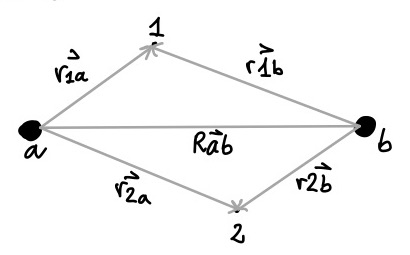
\includegraphics[scale=0.30]{img_8}
	\caption{A representation of the $H_2$ molecule given the Born-Oppenheimer approximation.}
	\label{fig:h2}
\end{figure}

	\subsection{Representation}
	The system can be firstly represented as two atoms at a large distance that approach slowly to each other, generating a linear combination of mean wave functions.
	The electrons are in a superposition of states when they start interacting, so the resulting H-H chemical bond is actually an entangled electron tunnelling.

	$$\psi(\vec{r_1},\vec{r_2},s_1^z,s_2^z,(\vec{R_a},\vec{R_b}))=\psi_{\text{spatial}}(\vec{r_1},\vec{r_2})\otimes\psi_{\text{spin}}(s_1^z,s_2^z)=\Phi\otimes\mathcal{X}$$

	The wave-function can be factorized, as the Hamiltonian is separable (i.e. does not depend on the spin).

	\subsection{Spin}
	Spins can be $\ket{\uparrow\uparrow}$, $\ket{\downarrow\downarrow}$, $\ket{\uparrow\downarrow}$, and $\ket{\downarrow\uparrow}$.
	Since electrons are fermions, the two spins' product must be antisymmetric, hence one of the two spins must be antisymmetric and the other one must be symmetric (the two possibilities are \textit{i}) spatial symmetry and spin antisymmetric, \textit{ii}) spatial antisymmetry and symmetric spin).
	Symmetry can be evaluated in entangled states, too.

	\begin{multicols}{2}
	\begin{itemize}
		 \item \textbf{Symmetric spin ($J=1$)}: $\ket{\uparrow\uparrow}$, $\ket{\downarrow\downarrow}$, $\frac{\ket{\uparrow\downarrow}+\ket{\downarrow\uparrow}}{\sqrt{2}}$ also called \textbf{triplet state} (quantum state of a system with a spin quantum number $s=1$), molecule bends in Stern-Gerlach.
		 \item \text{Antisymmetric spin ($J=0$)}: $\frac{\ket{\uparrow\downarrow}-\ket{\downarrow\uparrow}}{\sqrt{2}}$ also called \textbf{singlet state} (total spin angular moment $s=0$), molecule doesn't bend in Stern-Gerlach.
	\end{itemize}
	\end{multicols}

	The result is that a combination of two spin-$\frac{1}{2}$ particles can carry a total spin of $1$ or $0$, depending on whether they occupy a triplet or singlet state.

	\subsection{Model}
	Now we can generate now a model through a variational ansatz:

	$$\psi=\Phi \mathcal{X}=\begin{cases}\psi_1=\Phi_S \mathcal{X}_A = \frac{1}{\sqrt{2}} \big(\varphi_a(r_{1a}) \varphi_b (r_{1b})+\varphi_a (r_{2a}) \varphi_b (r_{2b})\big) \otimes\frac{\ket{\uparrow\downarrow}-\ket{\downarrow\uparrow}}{\sqrt{2}}\\\psi_2=\Phi_A\mathcal{X}_S = \frac{1}{\sqrt{2}} \big(\varphi_a(r_{1a}) \varphi_b (r_{1b})+\varphi_a (r_{2a}) \varphi_b (r_{2b})\big) \otimes\frac{\ket{\uparrow\downarrow}+\ket{\downarrow\uparrow}}{\sqrt{2}}\\\end{cases}$$

	The latter is a mean field model where E1 lives in P1 and E2 lives in P2.
	By the variational principle, the wavefunction with the lowest value of energy is the one that best approximates the H$_2$ atom.

	$$\hat{H}=-\frac{\hbar^2}{2m}\nabla_n^2-\frac{\hbar^2}{2m}\nabla_e^2-\frac{e^2}{|r_1a|}-\frac{e^2}{|r_1b|}-\frac{e^2}{|r_2a|}-\frac{e^2}{|r_2b|}-\frac{e^2}{|R_ab|}$$

	Even if spin is not involved in the Hamiltonian and eventually results in $\braket{\hat{S}}{\hat{S}}=1$, the sign of the expected value of the Hamiltonian depends on the spin symmetry, because spatial value and spin symmetry are entangled.

	\begin{multicols}{2}
		\begin{itemize}
			\item $E_1=\langle{\psi_1\,|\,\hat{H}\,|\,\psi_1}\rangle =\langle{\Phi_S\,|\,\hat{H}\,|\,\Phi_S}\rangle$
			\item $E_2=\langle{\psi_2\,|\,\hat{H}\,|\,\psi_2}\rangle=\langle{\Phi_A\,|\,\hat{H}\,|\,\Phi_A}\rangle$
		\end{itemize}
	\end{multicols}

	We must solve, then,

	$$E_1=\frac{1}{2}\int d\vec{r_1}\int d\vec{r_2}\,\big[\varphi(|\vec{r_1}-\vec{R_a}|)\varphi(|\vec{r_2}-\vec{R_b}|)+\varphi(|\vec{r_1}-\vec{R_b}|)\varphi(|\vec{r_2}-\vec{R_a}|)\big](\hat{H})(\Phi_S)$$

	And same for $E_2$.
	I have two 6-dimensions functions in 6-dimensions integrals.
	Results are different whether I solve for the first or second electron.

		\subsubsection{Distance of the atoms}
		This is the result that is obtained when the two atoms are infinitely far.

		$$\braket{\,|\,\hat{H}\,|\,}_{S/A}=2E_0\pm\text{stuff}$$

		Else, if the two atoms start to approach,

		$$\braket{\,|\,\hat{H}\,|\,}_{S/A}=\frac{e^2}{R_{ab}}\pm\text{separated ground states}$$

	\subsection{Results}
	We obtain two different functions, depicted in figure \ref{fig:variational}:

	\begin{multicols}{2}
	\begin{itemize}
		\item \textbf{Symmetric spatial function}: spin $0$ state, has a lower energy value that corresponds to an optimal distance between the two nuclei $\bar{R}$.
	It allows different calculable energy levels, bond oscillations and strength.
	Important to notice is that \textbf{quantum symmetry} (state $s=0$) is key to the binding of atoms.
		\item \textbf{Antisymmetric spatial function}: goes against the variational approximation, but technically is a right solution from a quantum mechanical point of view.
	\end{itemize}
	\end{multicols}

	\begin{figure}[htbp!]
		\centering
		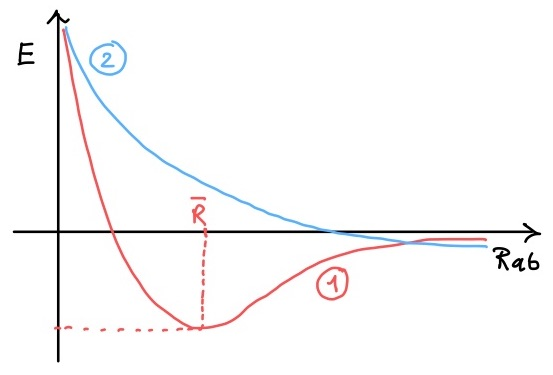
\includegraphics[scale=0.30]{img_9}
		\caption{The total energy is: $|E \rangle = \langle \psi | H | \psi \rangle = 2E_0 + \frac{e^2}{R_{ab}} \text{+ other factors}$.
							$E_0$ corresponds tot the energy of two atoms infinitely far away from each others, while $\frac{e^2}{R_{ab}}$ acts when the two atoms start to approach.}
		\label{fig:variational}
	\end{figure}

\section{Electronic structure calculation methods}
When choosing the best method to obtain an electronic structure, some evaluations have to be made regarding the accuracy of the calculation vs the computational cost of the operation.
The first approximation to be chosen is always the most important, as it determines the further steps that need to be taken.

\begin{figure}[htbp!]
	\centering
	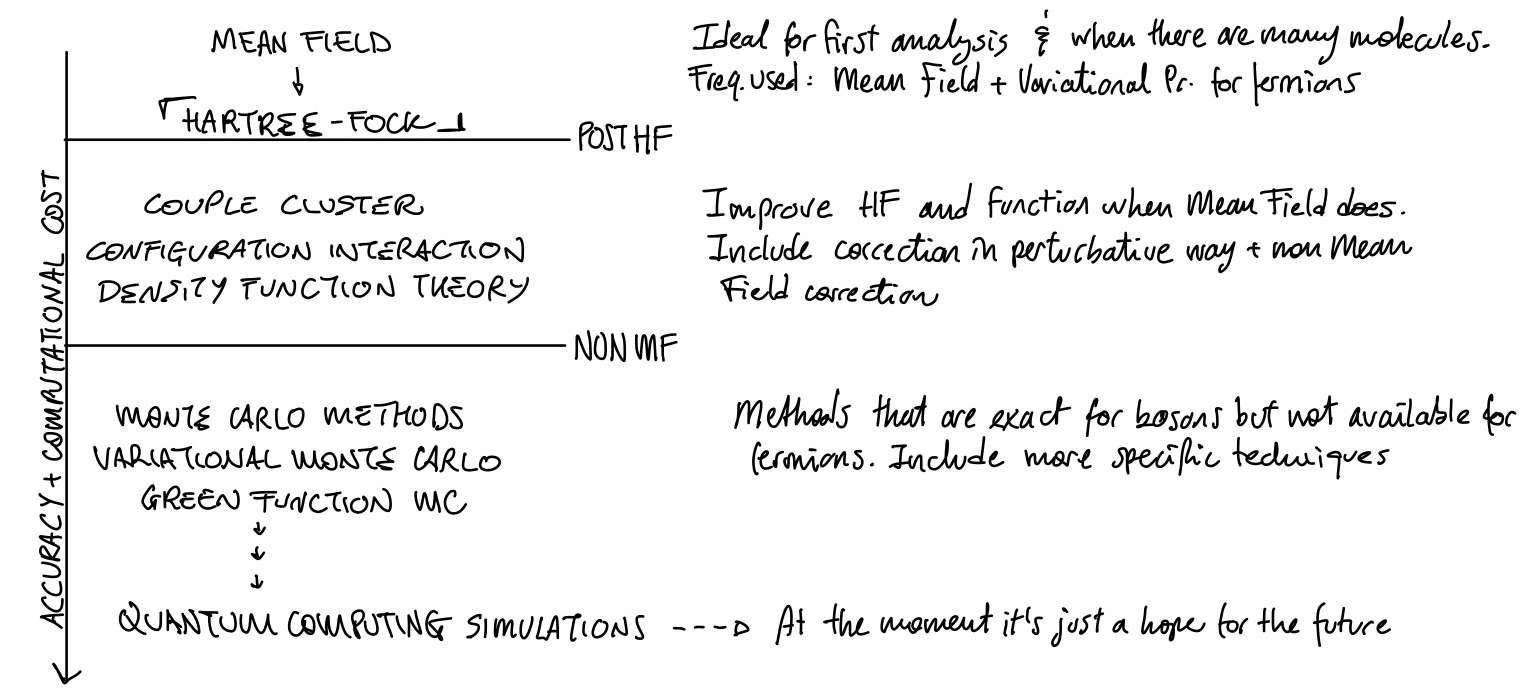
\includegraphics[scale=0.30]{img_13}
\end{figure}

	\subsection{Exact Diagonalization}
	The exact diagonalization with truncated basis technique is very precise, but it can't be used with system with more than 5 or 6 particles at the same time.
	For biological system, chemical accuracy is important as long as the error is not dramatic (keep in mind that a slight change of temperature can drastically change the system).
	A simulation is acceptable when $K_BT < 1.5\text{ KJ/mol} \div 2.4 \text{ KJ/mol}$.
	For macromolecules in biology, very accurate DFT are performed.
	The problem is that it's very difficult to predict Van Der Waals forces, since they are polynomial and DFT employs exponentials.
	The general goal is using classical equations to predict quantum-mechanics-descripted movements.

	\subsection{Hartree-Fock Method}
	Hartree-Fock method is a method of approximation for the determination of the wave function and the energy of a quantum many-body system in a stationary state that combines Mean Field Approximation, Fermi symmetry, and the Variational Principle.

		\subsubsection{Slater matrix}
		The method uses the Slater matrix's determinant to approximate a set of $N$ fermions.

		$$\psi(q_1\cdots q_n)=\frac{1}{\sqrt{2}}\begin{pmatrix}\phi_1(r_1)&\cdots&\phi_n(r_1)\\\cdots & &\cdots\\\phi_1(r_m)&\cdots&\phi_n(r_m)\end{pmatrix}$$

		We do not expect to find $\psi(q_1\cdots q_n)$.
		We can say it is the result of an equation and calculate the energy by using the Variational Principle with $E=\braket{\psi\,|\,E\,|\,\psi}$ and minimize $E$ with respect to $\psi(q)$ (a single-particle function) under the constraint of normalization ($\braket{\psi\,|\,\psi}=1$).
		Constraint minimization is operated with \textbf{Lagrange multipliers}: I consider a system of equations $f(x_1\cdots x_n)$ where I can calculate the minimum and the maximum with the application of the gradient $\nabla f=0$.

		\subsubsection{Hartree equation}
		We eventually obtain the \textbf{Hartree Equation}, representing \ul{one electron interacting with a probability cloud}.
		It is a symmetric system (valid for bosons, since they have classical limits and can be represented as shown without further additions):

		$$\bigg(-\frac{\hbar^2}{2m}\nabla^2_i-\frac{Z}{r_i}\bigg)\Phi_\lambda(\vec{r_i})+\sum_\mu \sum_{j \neq i} \int\,d^3\vec{r_j}\bigg(\Phi^*_\mu(\vec{r_j})\Phi_\mu(\vec{r_j})\frac{1}{|r_i-r_j|}\Phi_\lambda(\vec{r_i})\bigg)=E\Phi_\lambda(\vec{r_i})$$

		In particular:

		\begin{multicols}{2}
			\begin{itemize}
				\item $-\frac{Z}{r_i}$ is the coulombic attraction for a single nucleus (atomic physics version)
				\item $\Phi_\lambda(\vec{r_i})$ represents orbital position of the electron + spin.
			The number of electrons is the number of equations that need to be solved
				\item $\mu$ is the orbital index that changes the wave function
				\item $\Phi^*_\mu(r_j)\Phi_\mu(r_j) = \rho_\mu^{(i)}(r_j)$ is the electron density + density of charge around it (probability density) with sum of all electrons in all orbitals ($\mu$)
			\end{itemize}
		\end{multicols}

		\subsubsection{Fock equation}
		The Fermi symmetry introduces the Slater determinant, that is also called \textbf{exchange term} (\textbf{Fock equation}).
		This introduction implies that I cannot bring two electrons with the same spin in the same orbital.
		The wave function collapses to zero and I have repulsion between the electrons.

		$$\text{HARTREE EQN}+\sum_\mu \sum_{j \neq i} \int\,d^3\vec{r_j}\bigg(\Phi^*_{\mathcolorbox{yellow}{\mu}}(\vec{r_j})\Phi_{\mathcolorbox{yellow}{\lambda}}(\vec{r_j})\frac{1}{|r_i-r_j|}\Phi_{\mathcolorbox{yellow}{\mu}}(\vec{r_i})\bigg)=E\Phi_\lambda(\vec{r_i})$$

		This implies that the electron density factor of Hartree equation is not present anymore, the two particles are in a different state.
		At the same time, $\Phi_\mu(r_i)$ becomes Fock's generalization exchange term for fermions.
		This equation though is non linear ($\Phi^3$), so many quantum mechanics properties can't be applied to HF.
		The computational cost doesn't change over the introduction of the exchange term, even if it has a three-dimensional integral.

		\subsubsection{Algorithm}
		Since the equation cannot be expanded on a different basis, self consisted methods must be used.
		These are iterative procedures operated until the function converges:

		\begin{multicols}{2}
			\begin{enumerate}
				\item (Guess) $\Phi^{(t)}_\lambda (\vec{r})$.
				\item Compute $\rho_\mu^{(1)}(\vec{r})$ and $\rho_\mu^{(2)}(\vec{r})$, as they are numerical values.
				\item Insert $\rho_\mu^{(1)}(\vec{r})$ and $\rho_\mu^{(2)}(\vec{r})$ into HF equation, resulting in a conventional linear Schr\"odinger equation.
				\item Solve HF equation and get a more accurate wave function $\Phi^{(t+1)}_\lambda (\vec{r})$.
				\item Let $\Phi^{(t)}_\lambda = \Phi^{(t+1)}_\lambda$.
				\item Repeat until convergence (typically a single minimum is present).
			\end{enumerate}
		\end{multicols}

		I can use self consistent fields to compute the Hartree-Fock equation, but they are computationally expensive because they make heavy use of parallel computing.
		The Hartree-Fock equation can be used with semi empirical methods with coefficients in front of direct and exchange terms, that can weight the two terms in order to better match the experimental results.
		The Hartree-Fock equation is usually employed to build the expansion of the eigenfunction or in quantum computing.

	\subsection{Density Function Theory (DFT)}
	Variational in principle can yield the exact result, but they needs heuristic input and approximation to be feasible.
	Over the made assumptions, it is possible to achieve excellent results.
	Simple inputs are required for the perfect compromise between accuracy and computational cost.

		\subsubsection{Density function computation}
		The density function theory is based on density function computation instead of the wave function computation.
		Let the density operator:

		$$\hat{\rho}(\vec{r})=\sum_{i=1}^{N_0}\delta(\vec{r}-\vec{r_i})$$

		Now, its expected value assuming $\braket{\psi\,|\,\psi}=1$:

		$$\braket{\psi\,|\,\hat{\rho}(\vec{r})\,|\,\psi}=\sum_i \int\,d\vec{r_1}...d\vec{r_{N_e}}\bigg(\psi^*(\vec{r_1}-\vec{r_{N_e}})\delta(\vec{r}-\vec{r_i})\psi(\vec{r_1}-\vec{r_{N_e}})\bigg)\braket{\psi\,|\,\hat{\rho}(\vec{r})\,|\,\psi}=n(\vec{r})$$

		Which is the probability of finding any electron at the point $r$.
		This concept is shown in the following picture,  where blue is low electron density and red is high electron density.

		\begin{figure}[htbp!]
			\centering
			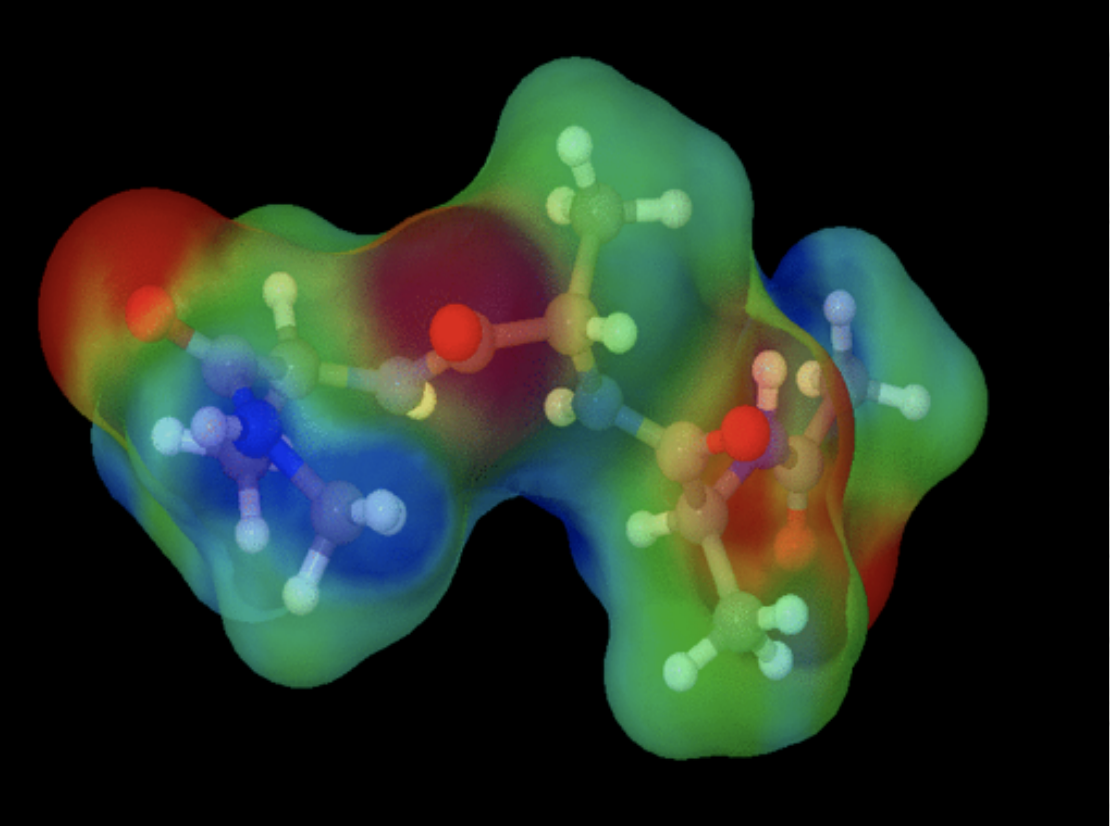
\includegraphics[scale=0.30]{img_14}
		\end{figure}

		\subsubsection{Single body density}
		$n(\vec{r})$ is a so-called single body density, representing different information with respect of the wave function (in fact $\hat{\rho}(\vec{r})$ reduces it when compared to $\psi$).
		For any Hamiltonian there is one and only single-body density.

		\subsubsection{Hochenberg and Kohn}
		Hochenberg and Kohn have elaborated two theorems that show that the ground state and excited states' properties of a system (quantum many-body system) are entirely determined by a single-body wave function $n(\vec{r})$.
		Mind that the quantum electronic structure calculation problem is:

		$$\hat{H}=-\frac{\hbar^2}{2m}\sum_i^{N_e}\nabla_i^2+\frac{1}{2}\sum_{i\neq j} \frac{e^2}{|r_i-r_j|}+\sum_i^{N_e}V_{ext}(\vec{r_i})$$

		The last term is the interaction between single electrons and nuclei.
		In the Born-Oppenheimer approximation, this was the external potential as nuclei were fixed.

			\paragraph{First theorem}
			For any system of interacting particles, the external potential is determined uniquely by the ground state one-body density.

			$$n_o(\vec{r})=\braket{\psi\,|\,\hat{\rho}(\vec{r})\,|\,\psi}$$

				\subparagraph{Corollary}
				All wave functions (ground state, first excited state and all eigenstates of $\hat{H}$) are fully determined by $n_0(\vec{r})$.

			\paragraph{Second theorem}
			A functional $E[n_0]$ can be defined such that the minimum of this functional with respect to $n_0(\vec{r})$ provides the exact $n_0(\vec{r})$ and $E_0$ (ground state energy).\\

		\subsubsection{Density function minimum}
		Given a function: $f: x \rightarrow f(x)$ where $x$ is a variable and $f(x)$ is a number), a functional $E[f]: f(x) \rightarrow E[f]$ is such where $f(x)$ is a function of operators and $E[f]$ is a number.
		Examples of functionals are definite integrals or the expectation values of operators.
		Ritz Theorem determines that the minimum of the functional of the wave function (the expectation value of the Hamiltonian) is the exact ground state.

			\paragraph{Solution}
			It is possible to define a functional such as the minimum of the functional is the exact value of the ground state energy.
			Differently from Ritz Theorem, the functional is not given and not referred to the wave function.
			The one body density functional minimum is the exact ground state energy of the problem for all the Hamiltonians.
			The theorems described above do not provide any solution, and they are usually complemented with ways to build the right functional to solve the problem.

\begin{figure}[htbp!]
	\centering
	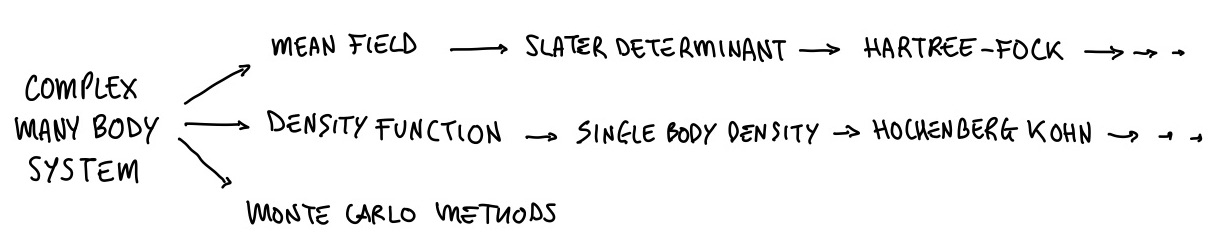
\includegraphics[scale=0.30]{img_15}
\end{figure}

	\subsection{QM-MM Schemes}
	QM-MM (Quantum mechanics - molecular mechanics) refers to hybrid systems used for large molecular models and chemical reactions studies like enzymatic reactions.
	Quantum mechanics is applied to the region of interest, while classical mechanics is used elsewhere.
	An hybrid method is used at the border of the two region of interest.
	This is done to focus the computational power strictly when needed, but still has problems when considering thermodynamics.


  \part{Quantum computing}

   \graphicspath{{chapters/08/}}
\chapter{Quantum computing}

\section{Qubits}
We can consider a quantum Hamiltonian $\hat{H_0}$ that describes a two-level system.
We can represent it with the same mathematical representation of spin even if it's not spin.
\begin{multicols}{2}
	\begin{itemize}
		\item $\ket{0}=\begin{pmatrix}1\\0\end{pmatrix}$
		\item $\ket{1}=\begin{pmatrix}0\\1\end{pmatrix}$
	\end{itemize}
\end{multicols}

With: $\hat{H_0}=-h\hat{\tau_x}$ and $\hat{\tau}_x$ Pauli matrix operator:

$$\hat{\tau_x}=\begin{pmatrix}0&1\\1&0\end{pmatrix}$$

Then:

$$\hat{H_0}=-h\begin{pmatrix}0&1\\1&0\end{pmatrix}$$

	\subsection{State of the Hamiltonian}
	The objective is to find:

	\begin{multicols}{2}
		\begin{itemize}
			\item$\ket{\hat{\Omega}}=\ket{\text{Ground state of }\hat{H_0}}$
			\item$\ket{\hat{\Sigma}}=\ket{\text{First excited state of }\hat{H_0}}$
		\end{itemize}
	\end{multicols}

	To find the possible states of the Hamiltonian first $\hat{H_0}\ket{\phi}=E\ket{\phi}$ is solved:

	\begin{align*}
		\det(H-\lambda \mathbb{1})&=0\\
		\det\begin{pmatrix}-\lambda&-h\\-h&-\lambda\end{pmatrix}&=0\\
		\lambda^2-h^2&=0 \rightarrow \lambda=\pm h
	\end{align*}

	$-h$ and $+h$ are the two possible energy eigenvalues and correspond to the ground state and first excited state, respectively.

		\subsubsection{Ground state}
		The ground state is computed: $E_\Omega=-h$

		$$\ket{\Omega}=\begin{pmatrix}a\\b\end{pmatrix}\rightarrow-h\begin{pmatrix}0&1\\1&0\end{pmatrix}\begin{pmatrix}a\\b\end{pmatrix}=-h\begin{pmatrix}a\\b\end{pmatrix}$$

		This is a two-variables system and can be resolved as such:

		$$\begin{cases}-ha=-ha\\-hb=-hb\end{cases}\rightarrow a=0\, \text{and}\, b=1\, \text{or}\, a=1\, \text{and}\, b=0$$

		$\ket{\Omega}$ can be rewrited as:

		$$\ket{\Omega}=\frac{1}{\sqrt{2}}\ket{1}+\frac{1}{\sqrt{2}}\ket{0}$$

		And since $\ket{1}=\begin{pmatrix}0\\1\end{pmatrix}$, the ket have to be normalized to get the $\begin{pmatrix}1\\1\end{pmatrix}$ that is the final result.
		$\ket{\Omega}$ is a quantum superposition of states.

		\subsubsection{First excited state}
		The first excited state: $E_\Sigma=+h$:

		$$[\ket{\Sigma}=\begin{pmatrix}a\\b\end{pmatrix}\rightarrow-h\begin{pmatrix}0&1\\1&0\end{pmatrix}\begin{pmatrix}a\\b\end{pmatrix}=+h\begin{pmatrix}a\\b\end{pmatrix}$$

		From this linear system we obtain the formulation for the first excited state.

		$$\ket{\Sigma}=\frac{1}{\sqrt{2}}\ket{1}-\frac{1}{\sqrt{2}}\ket{0}$$

		\subsubsection{Conclusion}
		Each of these two quantum states, $\ket{\Omega}$ and $\ket{\Sigma}$, represent a \textbf{qubit} that is in a linear superposition of states.\\

\subsection{Adiabatic Quantum Computing}
Putting energy in the system changes the probability of the particle of being still in a ground state.
The particle may be found in an excited state.
This doesn't happen if the system is switched in a slow manner and becomes an adiabatic system.
Doing so, according to the adiabatic system the system never ends up in an excited state and the transition is more likely to occur at time when $\Delta E$ is at its lowest.

	\subsubsection{Ground state of an arbitrary complex Hamiltonian}
	If $\hat{H_f}$ is complicated enough such that its ground state cannot be known, starting from $\hat{H_0}$ ground state and letting the system evolve in an adiabatic way to reach $\hat{H_f}$, $\hat{H_f}$ will reach the ground state spontaneously.
	Measuring the final state many times allows to discover the ground state of $\hat{H_f}$.

	\subsubsection{Final wave function through qubits}
	The final wavefunction can be obtained by means of qubits.
	Qubits are two level-systems that can thus have two levels of energy for which the two ground states are known.

\begin{figure}[htbp!]
	\centering
	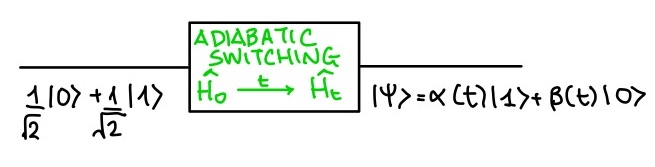
\includegraphics[scale=0.30]{img_10}
\end{figure}

The final solution can be computed by knowing the amount of values of $\alpha(t)$ and $\beta(t)$.
The time needed for the computation depends on:

\begin{multicols}{2}
	\begin{itemize}
		\item Triviality of the problem.
		\item The number of qubits $(n)$.
		\item The number of states ($2^n$).
		\item $\Delta E$.
	\end{itemize}
\end{multicols}

The time of computation depends on the function that regulated $\Delta E$ and corresponds to the clock of classical computers.

\section{Two qubits system}
Two qubits systems are interacting quantum systems.

	\subsection{Hamiltonian}
	The objective is to solve the Hamiltonian in the form:

	$$\hat{H}=\mathbf{J}_{12}\hat{\tau_1^z}\hat{\tau_2^z}+h(\hat{\tau_1^z}+\hat{\tau_2^z})$$

	This is a two-particles Hamiltonian that depends on the interaction of the two spins.
	If one of the two is down, $\hat{H}$ becomes negative and the energy is lowered.
	Hence I have a more favourable system.
	This can be obtained with a magnet that can properly align spins in order to have an overall negative energy.
	Implicitly, the Hamiltonian should be:

	$$\hat{H}=\mathbf{J}_{12}\hat{\tau_1^z}\hat{\tau_2^z}+h(\hat{\tau_1^z}\hat{\mathbb{1}_z}+\hat{\mathbb{1}_z}\hat{\tau_2^z})$$

	When using an operator on a particle, the other is multiplied by the identity matrix.

	$$\hat{\tau_1^z}\otimes\hat{\tau_2^z}=\begin{pmatrix}1&0&0&0\\0&-1&0&0\\0&0&-1&0\\0&0&0&1\end{pmatrix}\\hat{\tau_1^z}\otimes\hat{\mathbb{1}_z}=\begin{pmatrix}1&0&0&0\\0&1&0&0\\0&0&-1&0\\0&0&0&-1\end{pmatrix}\hat{\mathbb{1}^z}\otimes\hat{\tau_2^z}=\begin{pmatrix}1&0&0&0\\0&-1&0&0\\0&0&1&0\\0&0&0&-1\end{pmatrix}$$

	The Hamiltonian then becomes:

	$$\hat{H}=\mathbf{J}_{12}\begin{pmatrix}1&0&0&0\\0&-1&0&0\\0&0&-1&0\\0&0&0&1\end{pmatrix}+h\begin{pmatrix}2&0&0&0\\0&0&0&0\\0&0&0&0\\0&0&0&-2\end{pmatrix}=\begin{pmatrix}\mathbf{J}_{12}+2h&0&0&0\\0&-\mathbf{J}_{12}&0&0\\0&0&-\mathbf{J}_{12}&0\\0&0&0&-2h+\mathbf{J}_{12}\end{pmatrix}$$

	Each of the eigenvalues of the matrix can represent an eigenvector.

	\subsection{Quadratic unconstrained binary optimization problem}
	Suppose we have a function defined as a quadratic function of binary variables:

	$$T=\sum_{i,j=1}^N O_{ij}x_ix_j+\sum_i^N U_ix_i \text{ with } x_i\in \{0,1\} \text{ and } O_{ij},U_i\in \mathbb{R}$$

	The problem is finding the configuration of binary variables that minimises $T$.
	This is a discrete optimization problem that is called \textbf{Quadratic Unconstrained Binary Optimization (QUBO)} problem.
	We can reduce the two-particle problem to a QUBO problem.
	By definition $\hat{\tau_i^z}=2x_i-1$.
	When \[\begin{matrix}x_i=0&\hat{\tau_i^z}=-1\\x_i=1&\hat{\tau_i^z}=+1 \end{matrix}\]
	We can write the function $T$ as

	$$T=\sum_{i,j=1}^N \mathbf{J_{ij}}\tau_i^z\tau_j^z+\sum_i^N h_i\tau_i^z$$

	That is similar to the original Hamiltonian.
	This is the total number of combination of $2^N$.
	Values of $T$ are encoded in the Hamiltonian.
	Results of finding the minimum of $T$ and $\hat{H}$ are the same because the minimum value of the ground state corresponds to the ground eigenstate.
	The qubits corresponding to the ground eigenstate (eigenvectors) can be obtained from classical $T$ but not as a superposition.

	\subsection{Entangled states}
	Entangled states can be created by imposing a different spin direction on the particles.

	$$\hat{H}=\mathbf{J}_{12}\hat{\tau_1^z}\hat{\tau_2^z}+h(\hat{\tau_1^x}\hat{\mathbb{1}_x}+\hat{\mathbb{1}_x}\hat{\tau_2^x})$$
	$$\hat{\tau_1^x}\otimes\hat{\mathbb{1}_x}=\begin{pmatrix}0&0&1&0\\0&0&0&1\\1&0&0&0\\0&1&0&0\end{pmatrix}\hat{\mathbb{1}^x}\otimes\hat{\tau_2^x}=\begin{pmatrix}0&1&0&0\\1&0&0&0\\0&0&0&1\\0&0&1&0\end{pmatrix}\hat{H}=\begin{pmatrix}\mathbf{J}_{12}&h&h&0\\h&-\mathbf{J}_{12}&0&h\\h&0&-\mathbf{J}_{12}&h\\0&h&h&\mathbf{J}_{12}\end{pmatrix}$$

	The ground state is a vector correspondent to

	$$\begin{pmatrix}1\\0\\-\frac{\sqrt{4h^2+\mathbf{J}^2}+\mathbf{J}}{2h}\\1 \end{pmatrix}=\ket{0\,0}-\frac{\sqrt{4h^2+\mathbf{J}^2}+\mathbf{J}}{2h}\ket{1\,0}+\ket{1\,1}$$

	Where $c=\frac{\sqrt{4h^2+\mathbf{J}^2}+\mathbf{J}}{2h}$.
	Let the normalization factor:

	$$\frac{(1^2+c^2+1^2)}{N}=1 \rightarrow N=2+c^2$$

	$$G.S.=\frac{1}{\sqrt{2+c^2}}(\ket{0\,0}-c\,\ket{1\,0}+\ket{1\,1})$$

	Fix $c=1$ so the ground state becomes:

	$$G.S.= \frac{1}{\sqrt{3}}(\ket{0\,0}-\ket{1\,0}+\ket{1\,1})$$

	Compute the probability for $q_2=1$.
	$q_2$ can appear in two different states:

	\begin{align*}
		P_{1 1}&=\frac{1}{3}(\braket{1\,1\,|\,0\,0}-\braket{1\,1\,|\,1\,0}+\braket{1\,1\,|\,1\,1})^2=\bigg(\frac{1}{\sqrt{3}}\bigg)^2=\frac{1}{3}\\
		P_{0 1}&=\frac{1}{3}(\braket{0\,1\,|\,0\,0}-\braket{0\,1\,|\,1\,0}+\braket{0\,1\,|\,1\,1})^2=0
	\end{align*}

	This latter state never appears.
	The state is overall entangled because if $q_1=0$ the wave function collapses into $q_2=0$.
	If $q_1=1$, $q_2$ doesn't collapse because it can be either $q_2=0$ or $q_2=1$ with $50\%$ probability.
	$q_2$ is in a linear superposition of states if $q_1=1$.

\section{Quantum circuits}
Quantum circuits are models for \textbf{quantum computation},
where a computation is a sequence of quantum gates, measurements, and initialization of qubits to known values.
Circuits are written such as the horizontal axis is time and they are read from left to right.
Horizontal lines represent qubits, doubled lines are classical bits.
The items that connect the elements represents the operations performed on qubits.

	\subsection{Elementary logic gates}
	The elementary logic gates are model of computation or physical electronic devise that implements a boolean function on one or more binary input.
	They are irreversible: the input cannot be recovered from the output.

	\subsection{Universaility}
	Quantum computers can achieve universality, the complete conversion of an input of an arbitrary set of items into a corresponding output.
	Usually in quantum computation the output is a rotation of the input, all the operations used to perform such rotation $f(x)$ on input $x$ can be expressed as a single unitary matrix, for example

	$$U=\sum_j\ket{f(x)}\bra{x}$$

	The ability to implement any unitary matrix would mean the achievement of universality in the sense of standard digital computers.
	A strictly physical example would be the simulation of the dynamics of a system, where the time evolution is the unitary matrix and the Hamiltonian is the associated hermitian matrix.
	Achieving any unitary matrix would therefore correspond to simulating any time evolution, and engineering the effects of any Hamiltonian.

	\subsection{Quantum logic gates}
	Quantum logic gates are reversible unitary transformations on at least one qubit.

		\subsubsection{Qubits}
A qubit (the quantized version of classical \textit{n}-bit space $\{0,1\}^n$) is the Hilbert space $H_{QB(n)}=L^2(\{0,1\}^2)$, that can be interpreted as a linear combination or superposition of classical bit strings.
$H_{QB(n)}$ is a vector space over the complex numbers of dimension $2^n$ and elements of this vector space are possible state of \textit{n}-qubits quantum registers.
Quantum logic gates require a reversible function called unitary mapping which is linear transformation of a complex inner product space that preserves the Hermitian inner product.

	\subsection{Types of quantum circuits}
	There are three main types of quantum circuits:

	\begin{multicols}{2}
		\begin{itemize}
		\item \textbf{Phase gate (S gate)}: single-qubit operation defined by the matrix $S=\begin{pmatrix}1&0\\0&i \end{pmatrix}$, it represents a $90^\circ$ rotation around the $z$-axis.
		\item \textbf{Hadamard gate}: single-qubit operation that maps the basis state $\ket{0}$ to $\frac{\ket{0}+\ket{1}}{\sqrt{2}}$ and $\ket{1}$ to $\frac{\ket{0}-\ket{1}}{\sqrt{2}}$ thus creates a superposition of the two basis states.
			It can be represented by the matrix $H=\frac{1}{\sqrt{2}}\begin{pmatrix} 1&1\\1&-1\end{pmatrix}$.
			It represents a $90^{\circ}$ rotation around the $y$-axis followed by a $180^{\circ}$ rotation around the $x$-axis.
		\item \textbf{CNOT gate}: two-qubit operation.
			The first qubit is the control qubit, the second qubit is the target qubit.
			This gate leaves the control qubit unchanged and performs a Pauli-X gate on the target qubit if control is $\ket{1}$.
			If control is $\ket{0}$ the target qubit is unchanged.
			The CNOT gate is represented by the matrix $C_{NOT} = \begin{pmatrix}1&0&0&0\\0&1&0&0\\0&0&0&1\\0&0&1&0 \end{pmatrix}$
		\end{itemize}
	\end{multicols}

	\begin{figure}[htbp!]
		\centering
		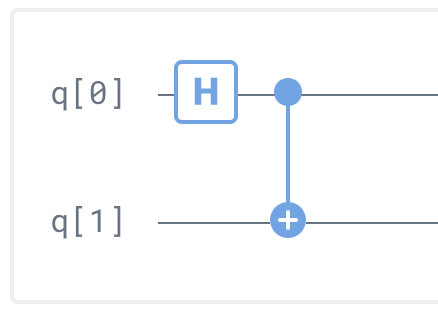
\includegraphics[scale=0.30]{img_11}
	\end{figure}

	The figure represents the execution of Hadamard gate on qubit 0 to create a superposition state and then the execution of CNOT gate to create an entangled state of the two qubits.

	\subsection{Prove that Hadamard gate is the reverse of itself}

	\begin{align*}
		H&=\frac{1}{\sqrt{2}}\begin{pmatrix}1&1\\1&-1\end{pmatrix}\,\,\ket{0}=\begin{pmatrix}1\\0\end{pmatrix}\,\,\ket{1}=\begin{pmatrix}0\\1\end{pmatrix}\\
		H\,\ket{0}&=\frac{1}{\sqrt{2}}\begin{pmatrix}1&1\\1&-1\end{pmatrix}\begin{pmatrix}1\\0\end{pmatrix}=\frac{1}{\sqrt{2}}\begin{pmatrix}1+0\\1+0\end{pmatrix}=\begin{pmatrix}1/\sqrt{2}\\1/\sqrt{2}\end{pmatrix}\\
		H\,(H\,\ket{0})&=\frac{1}{\sqrt{2}}\begin{pmatrix}1&1\\1&-1\end{pmatrix}\begin{pmatrix}1/\sqrt{2}\\1/\sqrt{2}\end{pmatrix}=\frac{1}{\sqrt{2}}\begin{pmatrix}1/\sqrt{2}+1/\sqrt{2}\\1/\sqrt{2}-1/\sqrt{2}\end{pmatrix}=\frac{1}{\sqrt{2}}\begin{pmatrix}2/\sqrt{2}\\0\end{pmatrix}=\begin{pmatrix}1\\0\end{pmatrix}
	\end{align*}

	It's pointless to put two Hadamard gates in a row from a mathematical point of view.
	From a physical point of view it means that I am restoring the cat in an aline/dear definite state that is technically not possible.

	\subsection{Example of a $HC_{NOT}$}
	Application of the two gates on different entangled states of qubits $\ket{0}$ and $\ket{1}$.

	\begin{align*}
		C_{NOT}(H\,\ket{0\,0})&=C_{NOT}(H\,\ket{0}\otimes\ket{0})=C_{NOT}\bigg(\frac{1}{\sqrt{2}}\begin{pmatrix}1&1\\1&-1\end{pmatrix}\begin{pmatrix}1\\0\end{pmatrix}\otimes\begin{pmatrix}1\\0\end{pmatrix}\bigg)=\\
													&=C_{NOT}\bigg(\frac{1}{\sqrt{2}}\begin{pmatrix}1\\1\end{pmatrix}\otimes\begin{pmatrix}1\\0\end{pmatrix}\bigg)=\\
													&=C_{NOT}\frac{1}{\sqrt{2}}\begin{pmatrix}1\\0\\\mathcolorbox{yellow}{1}\\\mathcolorbox{yellow}{0}\end{pmatrix}=\frac{1}{\sqrt{2}}\begin{pmatrix}1&0&0&0\\0&1&0&0\\0&0&0&1\\0&0&1&0\end{pmatrix}\begin{pmatrix}1\\0\\1\\0\end{pmatrix}=\\
													&=\frac{1}{\sqrt{2}}\begin{pmatrix}1+0+0+0\\0+0+0+0\\0+0+0+0\\0+0+1+0\end{pmatrix}=\frac{1}{\sqrt{2}}\begin{pmatrix}1\\0\\\mathcolorbox{yellow}{0}\\\mathcolorbox{yellow}{1}\end{pmatrix}=\\
													&=\frac{\ket{0\,0}+\ket{1\,1}}{\sqrt{2}}=\ket{\phi^+}
	\end{align*}
	As foreseen in the theory, the second qubit changes when the $C_{NOT}$ gate is applied.
	The result is an entangled state of the two qubits called Bell state.
	All Bell states resulting from the combinations are orthogonal to each other.

	$$\frac{\ket{0\,0}-\ket{1\,1}}{\sqrt{2}}=\ket{\phi^-}\,\,\frac{\ket{0\,1}+\ket{1\,0}}{\sqrt{2}}=\ket{\psi^+}\,\,\frac{\ket{0\,1}-\ket{1\,0}}{\sqrt{2}}=\ket{\psi^-}$$

	$$\braket{\psi^+\,|\,\psi^-}=0$$

\section{The Elitzur-Vaidman bomb tester}
The Elitzur-Vaidman bomb tester is a quantum mechanics thought experiment that uses interaction-free mechanism to verify that a bomb is functional without having to detonate it.
This experiment uses two characteristics of elementary particles: \textbf{nonlocality} and \textbf{wave-particle duality}.
The fundamentals of this experiment can be explained with an example: if we have two closed boxes and we know that in one of the two there is an object, by opening one and finding it empty, we know that the object is in the other one without opening it.
The particle, during the experiment, is in a superposition of states/locations, it can be anywhere in any moment.
The particle's wave can be collapsed by observing it to obtain its local information.
Information about previous positions of the particle can be obtained before the collapse and even in cases where the particle was never in those positions.

\begin{figure}[htbp!]
	\centering
	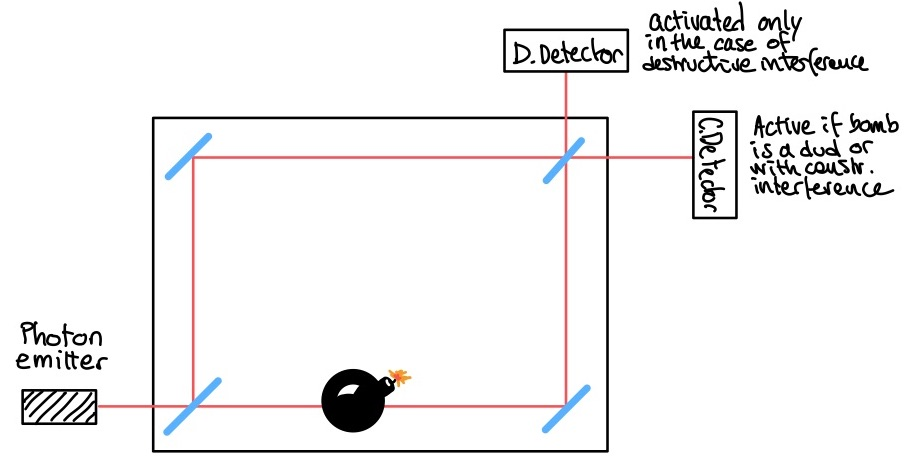
\includegraphics[scale=0.30]{img_12}
\end{figure}


	\subsection{Bomb not inserted}
When the photon is emitted and it reaches the first beam splitter, a superposition of states is created, the photon can either go to the upper path or to the lower path with a $50\%$ probability each.
The photon encounters two mirrors that reflect the beam and the two meet at a second beam splitter that directs the beam to two detectors with the same probability:

\begin{multicols}{2}
	\begin{itemize}
		\item C Detector: reached by the transmitted beam.
	Activated by the constructive interference of the two photons behaving as waves.
		\item D Detector: reached by the reflected beam.
	Never activated in normal conditions (destructive interference happens hence no signal)
	\end{itemize}
\end{multicols}

	\subsection{Dud bomb}
	When the bomb is dud, $C$ detector has a $100\%$ probability of detecting a signal.
	The superposition of states created by the first beam splitter create a constructive interference that is detected by $C$.
	In $D$ there is destructive interference so nothing is detected.

	\subsection{Bomb inserted and live}
	Three things may happen when the bomb is inserted and live:

	\begin{multicols}{2}
		\begin{itemize}
			\item $50\%$ the bomb explodes: The photon took the lower path and activated the bomb.
				The activation of the bomb can be considered as a collapse of the wave function, the photon never arrives at the detector and no signal is present.
			\item $25\%$ photon detected at $C$: The photon took the upper way and was transmitted by the second beam splitter.
			\item $25\%$ photon detected at $D$: The photon took the upper way and was reflected by the second beam splitter.
				The presence of a signal at detector $D$ is the only way to know whether the bomb is live without its explosion.
		\end{itemize}
	\end{multicols}


  \part{Mathematical Background}

    \chapter{Complex numbers}
A broad range of problems can be solved within real numbers, however it is easy to find some that are not solvable in $\mathbb{R}$.
For example the equation $x^2+1=0$ has no solution in the real numbers.
Because of this reason, the real number set is extended, trying to develop a coherent framework in which these problems can be solved.
Following this procedure a new variable $i$ is defined, such that:

$$i := \sqrt{-1}\not\in\mathbb{R}$$

This quantity is called the imaginary unit and it is used to define a new kind of numbers or complex numbers, defined in standard form as:

$$z := \underbrace{a}_{\text{Real part, }\Re{z}} + \underbrace{bi}_{\text{Imaginary part, }\Im{z}}$$

Where $a\land b\in\mathbb{R}$.
Thus we can define a new set of numbers $\mathbb{C}$ such that $z\in\mathbb{C}$ and $\mathbb{R}\subset\mathbb{C}$.
In fact any real number is a complex number where $b=0$.

\section{Argand plane}
Complex numbers can be seen as ordered pairs of reals and they can be naturally plotted on the complex or argand plane.
The horizontal direction represents the real axis while the vertical one represents the imaginary one.

\section{Operations}

	\subsection{Addition}
	Let $z, w\in\mathbb{C}$ be two complex numbers such that $z = a+bi$ and $w = c+di$, where $a,b,c,d\in\mathbb{R}$.
	The addition is defined as:

	$$z+w = (a+c) + (b+d)i$$

	\subsection{Subtraction}
	Let $z, w\in\mathbb{C}$ be two complex numbers such that $z = a+bi$ and $w = c+di$, where $a,b,c,d\in\mathbb{R}$.
	The subtraction is defined as:

	$$z-w = (a-c) + (b-d)i$$

	\subsection{Multiplication}
	Let $z, w\in\mathbb{C}$ be two complex numbers such that $z = a+bi$ and $w = c+di$, where $a,b,c,d\in\mathbb{R}$.
	Remembering that $i^2 = -1$, the multiplication of two complex number is:

	\begin{align*}
		z\cdot w &= (a+bi)(c+di) = \\
						 &=ac+adi+bci+bdi^2 =\\
						 &= ac+(ad+bc)i -bd =\\
						 &= (ac-bd)+(ad+bc)i
	\end{align*}

	\subsection{Complex conjugate}
	Let $z\in\mathbb{C}$ be a complex number such that $z=a+bi$, where $a,b\in\mathbb{R}$.
	The complex conjugate is defined as:

	$$z^*=a-bi$$

	So we take the opposite of the imaginary part.

	\subsection{Division}
	Let $z, w\in\mathbb{C}$ be two complex numbers such that $z = a+bi$ and $w = c+di$, where $a,b,c,d\in\mathbb{R}$.
	The complex conjugate can be used to define a division operation that brings the result in standard form.
	The operation is similar to the rationalization of a fraction: the nominator and the denominator are multiplied by the complex conjugate of the denominator.
	This is because the product of a complex number and its conjugate is always real.
	So the division is defined as:

	\begin{align*}
		\frac{z}{w} &= \frac{a+bi}{c+di} = \\
								&=\frac{a+bi}{c+di}\frac{c-di}{c-di}=\\
								&=\frac{ac - adi + bci +bd}{c^2+d^2}=\\
								&= \frac{(ac + bd) + (bc - ad)i}{c^2+d^2} = \\
								&=\frac{ac +bd}{c^2+d^2} + \frac{bc-ad}{c^2+d^2}i
	\end{align*}

\section{Polar form}

	\subsection{Complex numbers as vectors}
	Complex numbers can be plotted as points in the Argand plane, using as coordinates the real and the imaginary parts.
	In this way a complex number can be seen as a vector of modulus:

	$$\rho = |z| = \sqrt{a^2+b^2}$$

	Due to Pitagora's theorem.
	Complex number are added and subctrated as such.

	\subsection{Definition}
	The polar form is useful to have a simple interpretation of multiplication and division and it is defined as:

	$$z :=\rho(\cos\theta + i\sin\theta)$$

	The variables used for this representation are the modulus $\rho$ and the argument $\theta$, the angle between the positive direction of the real axis and the vector itself.
	The modulus of a complex number is always positive.
	Complex numbers in polar form are periodic with the argument $\theta$ with periodicity $2k\pi$, $\forall k\in\mathbb{Z}$.

	\subsection{Conversion between polar form and standard form}
	Any complex number written in standard form can be written in polar form, where:

	$$\begin{cases}
		\theta = \arctan \frac{b}{a}\\
		\rho = \sqrt{a^2 + b^2}
	\end{cases}$$

	Likewise, you can pass from polar form to standard form using:

	$$\begin{cases}
		a = \rho\cos\theta\\
		b = \rho\sin\theta
	\end{cases}$$
   
	\subsection{Operations}

		\subsubsection{Multiplication}
		Let $z, w\in\mathbb{C}$ be two complex numbers such that $z = \rho_z(\cos\theta_z + i\sin\theta_z)$ and $w = \rho_w(\cos\theta_w + i\sin\theta_w)$.
		The multiplication between $w$ and $z$ is:

		\begin{align*}
			zw &= \rho_z\rho_w(\cos\theta_z +i \sin\theta_z)(\cos\theta_w +i \sin\theta_w) =\\
				 &= \rho_z\rho_w[\cos\theta_z\cos\theta_w - \sin\theta_z\sin\theta_w + i(\sin\theta_z\cos\theta_w + \cos\theta_z\sin\theta_w)]
		\end{align*}

		Using now the addition formulas for cosine and sine:

		$$zw = \rho_z\rho_q[\cos(\theta_z+\theta_w) + i\sin(\theta_z+\theta_w)]$$

		\subsubsection{Division}
		Let $z, w\in\mathbb{C}$ be two complex numbers such that $z = \rho_z(\cos\theta_z + i\sin\theta_z)$ and $w = \rho_w(\cos\theta_w + i\sin\theta_w)$.
		In a similar way as the multiplication, the division will be:

		$$\frac{z}{w} = \frac{r_z}{r_w}[\cos(\theta_z-\theta_w) + i\sin(\theta_z-\theta_q)]$$

		\subsubsection{Power}
		According to the de Moivre theorem, for every $n\in\mathbb{N}$ positive integer and $z\in\mathbb{C}$, where $z = \rho(\cos\theta + i\sin\theta)$:

		$$z^n = \rho^n(\cos n\theta + i\sin n\theta)$$

		\subsubsection{N-th root}
		For every $n\in\mathbb{N}$ positive integer and $z\in\mathbb{C}, z = \rho(\cos\theta + i\sin\theta)$:

		$$\sqrt[n]{z} = \rho^{\frac{1}{n}}\biggl[\cos\biggl(\frac{\theta+2k\pi}{n}\biggr) + i\sin\biggl(\frac{\theta+2k\pi}{n}\biggr)\biggr]$$

		Where $k$ is an integer.
		Note that $k$ and $k=k+n$ produce identical solutions, so $k$ can be limited to the set $\{0,1,\dots, n-1\}$.
		In conclusion there are $n$ distinct roots, each with modulus $r^{\frac{1}{n}}$, that when represented together on the Argand plane lie on the circle of radius $\rho$. The roots are equally spaced and they create a regular polygon when joined.

\section{Complex valued functions}
Real functions can be extended to complex valued functions.
Taken $f$ from an interval $A\subset\mathbb{R}$ to $\mathbb{C}$, the function can then be written as:

$$f(x) = u(x) + v(x)i$$

Where $u$ and $v$ are real valued functions.
The limit of a complex valued function exists if the limits of the real and the complex component exist.
    
    \subsection{Complex conjugate}
    The complex conjugate of a composite function propagates through each of the components, meaning you have to change the sign before each imaginary unit $i$. For example:

    $$(\sin(ix) + ie^{3x + 2i})^* = (\sin(ix))^* + (ie^{3x + 2i})^* = \sin(-ix) - ie^{3x - 2i}$$

	\subsection{Derivative}
	The derivative of a complex valued function is obtained differentiating its real and imaginary parts:

	$$f'(x) = u'(x) + v'(x)$$

	The properties of the derivatives can be extended to this case: if $f$ and $g$ are two complex valued functions differentiable at some point $x_0$ in the domain of both functions, $f\pm g$, $fg$ and $\frac{f}{g}$ ($g(x_0)\neq 0$) are differentiable and the values of these functions are, just like in the real case:

	$$(f\pm g)'(x_0) = f'(x_0) + g'(x_0)$$

	$$(fg)'(x_0) = f'(x_0)g(x_0) + f(x_0)g'(x_0)$$

	$$\frac{f}{g}'(x_0) = \frac{f'(x_0)g(x_0)-f(x_0)g'(x_0)}{g^2(x_0)}$$

\section{Complex exponential}
Due to its properties and applications it is desirable to extend the exponential function to the complex field.
A complex exponential function is in the form $e^{a+bi}$.
From the case $a = 0$:

$$e^{ti} = \cos t + i\sin t$$

If $a, b\neq 0$;

\begin{align*}
	e^{a+bi} &= e^ae^{bi} =\\
					 &=e^a(\cos b + i\sin b)
\end{align*}

	\subsection{Properties}
	Not only the product of two complex exponentials meets the classical properties of the real exponentials, the derivatives maintains them too.
	Let $t\in\mathbb{R}$ and $y(t) = e^{(a+bi)t} = e^{at}(\cos t b + i\sin b)$, its derivative with respecto to $t$ is:

	\begin{align*}
		\frac{dy(t)}{dt} &= \frac{de^{(a+bi)t}}{dt}=\\
										 &= (a+bi)e^{(a+bi)t}
	\end{align*}

	It can be demonstrated that given $z\in\mathbb{C}$, $\frac{de^z}{dz} = e^z$.

	\subsection{Roots of a complex number}
	The complex exponential allows to write the $n$ roots of a complex number $z = r(\cos\theta + i\sin\theta)$ as:

	$$w_k = r^\frac{1}{n}e^{i\frac{\theta+2kn}{n}}$$

	Where $k\in\{0, 1, \dots, n-1\}$.

    \chapter{Partial derivatives}

\section{First order derivatives}
The concept of derivative can be used to explore function of $n\ge 2$ variables.
Let $f:\mathbb{R}^2\supseteq A\rightarrow \mathbb{R}$, where $A$ is an open set of $\mathbb{R}^2$ a function of two variables: $f(x, y)$.
The partial derivative of $f(x,y)$ with respect to $x$ in the point $(x_0, y_0)$ is defined as:

$$\frac{\partial f(x_0, y_0)}{\partial x} := \lim\limits_{h\rightarrow 0}\frac{f(x_0+h, y_0) -f(x_0, y_0)}{h}$$

With $h\in\mathbb{R}$ when the limit exists.
Equivalently the partial derivative of $f(x, y)$ with respect to $y$ in $(x_0, y_0)$ is:

$$\frac{\partial f(x_0, y_0)}{\partial y} := \lim\limits_{h\rightarrow 0}\frac{f(x_0, y_0+h) -f(x_0, y_0)}{h}$$

With $h\in\mathbb{R}$ when the limit exists.
That is the derivative of $f(x,y)$ with respect to a variable is computed as if other variables are held constant.
The existence of the partial derivative with respect to one variable does not imply the existence of the partial derivatives along any other direction.
The derivative along a general direction $\vec{v}$ is called directional derivative and is defined as:

$$D_{\vec{v}}f(x_0, y_0) := \lim\limits_{t\rightarrow 0}\frac{f((x_0, y_0) + t\vec{v}) - f(x_0, y_0)}{t}$$

With $t\in\mathbb{R}$ where the limit exists.

	\subsection{Differentiability}
	The concept of differentiability is introduced because the existence of the derivative along one direction does not imply the existence of directional derivatives along different directions.
	Let $\mathbb{R}^2\supseteq A\rightarrow\mathbb{R}$, with $A$ an open set of $\mathbb{R}^2$, a function of two variables $f(x,y)$ is differentiable if the partial derivatives exist in $(x_0, y_0)$ and:

	$$\lim\limits_{*h,k)\rightarrow(0,0)}\frac{f(x_0+h, y_0+k) - f_x(x_0, y_0)h - f_y(x_0, y_0)k}{\sqrt{h^2+k^2}} = 0$$

	Where $f_x$ and $f_y$ are the partial derivative with respect to $x$ or $y$.

	\subsection{Tangent plane}
	The tangent plane of $f(x,y)$ in the point $(x_0, y_0)$ has the following form:

	$$g(x,y) = f(x_0, y_0) + f_x(x_0, y_0)(x-x_0) + f_y(x_0, y_0)(y-y_0)$$

	\subsection{Determine if a function is differentiable}
	A function if differentiable in a point if the following condition holds true.
	Let $f:\mathbb{R}^2\supseteq A\rightarrow \mathbb{R}$ with $A$ an open set of $\mathbb{R}^2$.
	If in a neighbourhood of $(x_o, y_0)$ all the partial derivatives of $f(x, y)$ exists and are continuous in $(x_0, y_0)$ then $f(x,y)$ are differentiable in $(x_0, y_0)$.
	If a function has all the partial derivatives in a point and they are continuous, the function is differentiable.
	That means that exists the tangent plane in that point.

\section{Higher order derivatives}
Let $f:\mathbb{R}^2\supseteq A\rightarrow\mathbb{R}$, with $A$ an open set of $\mathbb{R}^2$, a function of two variables $f(x,y)$.
Supposing that the partial derivatives exist in a neighbourhood $I$ of $(x_0, y_0($, the two functions $g(x,y) = \frac{\partial f(x,y)}{dx}:\mathbb{R}^2\supseteq I\rightarrow\mathbb{R}$ and $h(x,y) = \frac{\partial f(x,y)}{dy}:\mathbb{R}^2\supseteq I\rightarrow\mathbb{R}$ can be seen as the analogous of $f$ and there is a possibility of taking the partial derivatives of $g$ and $h$ in a point $(x_0, y_0)$.
This means applying the $g$ and $h$ the operators $\frac{\partial }{\partial x}$ and $\frac{\partial}{\partial y}$.
The second order derivatives are defined as:

\begin{table}[H]
	\begin{tabular}{c c}
		$\frac{\partial^2 f}{\partial x^2}: \frac{\partial}{\partial x}g = \frac{\partial}{\partial x}\frac{\partial f}{\partial x}$ &
		 $\frac{\partial^2 f}{\partial y\partial x}: \frac{\partial}{\partial y}g = \frac{\partial}{\partial y}\frac{\partial f}{\partial x}$ \\
		$\frac{\partial^2 f}{\partial x\partial y}: \frac{\partial}{\partial x}h = \frac{\partial}{\partial x}\frac{\partial f}{\partial y}$ &
		 $\frac{\partial^2 f}{\partial y^2}: \frac{\partial}{\partial y}h = \frac{\partial}{\partial y}\frac{\partial f}{\partial y}$\\
	\end{tabular}
	\centering
\end{table}

When the partial derivative is taken two times in the same direction the second partial derivatives are named pures, when is taken along a different direction with respect to the first time they are named mixed.

	\subsection{Schwartz's theorem}
	Let $f(x, y)$ be a function defined in $\mathbb{R}^2$ and $I$ a neighbourhood of $(x_0, y_0)$ and $\partial x\partial y f$ and $\partial y\partial x f$ be continuous in $I$, then:

	$$\frac{\partial^2 f}{\partial x\partial y} = \frac{\partial ^2 f}{\partial y\partial x}$$

	All of this can be extended to higher order partial derivatives and to functions from $\mathbb{R^n}$ to $\mathbb{R}$ with an increasing number of combinations of derivatives.
	This theorem is useful form many reasons, one of which the fact that if the four order mixed partial derivatives are continuous at $(x_0, y_0)$ the order of the first order partial derivatives can be rearranged as preferred.

    \chapter{Differential operators}

\section{Definition}
An operator is a mapping of a certain set of structured objects such as a functions onto itself:

$$\hat{A}\cdot f = g$$

Operators can map functions to function or vectors to vectors.
These two cases are conceptually the same, because functions are elements of a vector space called the Hilbert space.
A differential operator is an operator which acts on functions and it is defined as some combination of differentiation operations.

\section{Properties}

	\subsection{Sum and difference}
	Given two operators $\hat{A}$ and $\hat{B}$ acting on some function $f$:

	$$(\hat{A} \pm\hat{B})f = \hat{A}f\pm \hat{B}f$$

	\subsection{Product}
	Given two operators $\hat{A}$ and $\hat{B}$ acting on some function $f$:

	$$(\hat{A}\hat{B})f = \hat{A}(\hat{B}f)$$

	Basically you apply the operators in subsequent order.

	\subsection{Power}
	Given an operator $\hat{A}$

	$$\hat{A}^n = \prod\limits_{i=1}^n\hat{A}$$

	\subsection{Equality}
	Given two operators $\hat{A}$ and $\hat{B}$ acting on some function $f$, they are defined equal if:

	$$\hat{A} = \hat{B} \Leftrightarrow \hat{A}f = \hat{B}f$$

	\subsection{Identity operator}
	The identity operator $\hat{1}$ is an operator such that:

	$$\hat{1}f = f$$

	\subsection{Commutability}
	Two operators are said to commute when the order of their consecutive application does not matter:

	$$\hat{A}\hat{B} = \hat{B}\hat{A}$$

	If this is the case their commutator is zero:

	$$[\hat{A}, \hat{B}] = \hat{A}\hat{B}-\hat{B}\hat{A} = 0$$

	Note that:

	$$\forall \hat{A}, \hat{B}: [\hat{A}, \hat{B}] = -[\hat{B}, \hat{A}]$$

	Two partial derivatives commute for $\mathbb{C}^2$ functions.

	\subsection{Linearity}
	Linear operators are operators which respect the property of linearity: given an operator $\hat{A}$ acting on $f$ and $g$, and given a constant multiplier $c$:

	$$\hat{A}(f\pm g) = \hat{A}f\pm \hat{A}g$$
	$$\hat{A}(cf) = c\hat{A}f$$

\section{Gradient, divergence and curl}

	\subsection{Nabla operator}
	The nabla operator defined in the $3D$ cartesian coordinate system is the $3$-component vector of partial derivatives over each axis:

	$$\vec{\nabla} = \begin{pmatrix} \frac{\partial}{\partial x} & \frac{\partial}{\partial y} & \frac{\partial}{\partial z}\end{pmatrix}$$

	The nabla operator is a linear differential operator which acts on functions and works as a $3D$ vector in space.

	\subsection{Scalar fields and vector fields}
	Single-valued functions of coordinate $f(\vec{x})$ are called scalar fields.
	They may represent a distribution of some density or the distribution of electrostatic charge in spece.
	$3D$ vectors which depend on coordinates, for example $3$-valued functions of coordinates $\vec{f}(\vec{x})$ are called vector fields.
	They can represent quantities such as currents flow in a fluid, or the electric and magnetic fields in space.

	\subsection{Gradient}
	Let $f:\mathbb{R}^3\supseteq A\rightarrow\mathbb{R}$, with $A$ an open set of $\mathbb{R}^3$, a function of three variables $f(x,y,z)$.
	Be the function derivable.
	The gradient of $f$ in Cartesian coordinates is defined as:

	$$\grad f = \nabla f := \frac{\partial f(x,y,z)}{\partial x}\hat{i} + 
							\frac{\partial f(x,y,z)}{\partial y}\hat{j} + 
							\frac{\partial f(x,y,z)}{\partial z}\hat{k}$$

	The gradient of a scalar function is defined as nabla acting on it and producing a vector field of its derivatives.
	The gradient is then the vector that takes as components along the axes directions the first order partial derivatives.
	The gradient is the vector of major increment of the function with respect to the variations in the variables and it has magnitude equal to the maximum rate of increase at the point.

		\subsubsection{Directional derivatives}
		Directional derivatives for $\mathbb{C}^1$ functions can be written as the scalar product of the gradient of the function and the vector $\vec{v}$:

		$$\vec{\nabla}_{\vec{v}}f(\vec{x}) = \vec{v}\vec{\nabla}f(\vec{x})$$

	\subsection{Divergence}
	Suppose now to have a derivable vectorial field $\vec{V}:\mathbb{R}^3\supseteq A \rightarrow\mathbb{R}^3$, with $A$ being an open set of $\mathbb{R}^3$.
	This vectorial field is defined by means of its components along the axes directions: $\vec{V} = v_1\hat{i} + v_2\hat{j} + v_3\hat{k}$.
	Basically, the vectorial field associates a vector to each point of $A$.
	The gradient, if it exists and if it is derivable, is a vectorial field.
	The divergence of $\vec{V}$ in Cartesian coordinates is:

	$$div\vec{V} = \nabla\cdot\vec{V} := \frac{\partial v_1(x,y,z)}{\partial x} + \frac{\partial v_2(x,y,z)}{\partial y} + \frac{\partial v_3(x,y,z)}{\partial z}$$

	It is thus defined as nabla acting on a vector field via the scalar product.
	This gives information on where a vectorial field has source or sink or, when the vectorial field represents a fluid flux, if the fluid is incompressible or solenoidal.

	\subsection{Curl}
	Suppose now to have a derivable vectorial field $\vec{V}:\mathbb{R}^3\supseteq A \rightarrow\mathbb{R}^3$, with $A$ an open set of $\mathbb{R}^3$.
	The application of the curl to $\vec{V}$ is:

	$$rot\vec{V} = \nabla\times\vec{V} := \biggl(\frac{\partial v_3}{\partial y} - \frac{\partial v_2}{\partial z}\biggr)\hat{i} + \biggl(\frac{\partial v_1}{\partial z} - \frac{\partial v_3}{\partial x}\biggr)\hat{j} + \biggl(\frac{\partial v_2}{\partial x} - \frac{\partial v_1}{\partial y}\biggr)\hat{k}$$

	It is thus defined as nabla acting on a vector field via the vector or cross product.
	The application of the curl to a vectorial field gives information on whether the field rotates around a point and on the verse of that rotation.
	The output of the curl is the modulus of the rotation, and the direction is linked by means of the right hand rule to the verse of rotation.

	\subsection{Properties}

	\begin{multicols}{3}
		\begin{itemize}
			\item $\nabla\times\nabla f = \vec{0}$
			\item $\nabla\cdot\nabla\times\vec{V} = 0$
			\item $\nabla\cdot f = \nabla^2 f$
		\end{itemize}
	\end{multicols}

	\subsection{Laplacian}
	The Laplacian is an operator defined as:

	$$\Delta f = \nabla^2 f = \frac{\partial^2}{\partial x^2}f + \frac{\partial^2}{\partial y^2}f + \frac{\partial^2}{\partial z^2}f$$

	It is the scalar product of two nabla operators.
	In spherical coordinates:

	$$\Delta f = \frac{1}{r^2}\frac{\partial}{\partial r}\biggl(r^2\frac{\partial}{\partial r}f\biggr) + \frac{1}{r^2\sin\theta}\frac{\partial}{\partial\theta}\biggl(\sin\theta\frac{\partial}{\partial\theta}f\biggr) + \frac{1}{r^2\sin^2\theta}\frac{\partial^2}{\partial\phi^2}f$$

\section{Hessian matrix: maxima and minima}
A matrix of $n$ order partial derivatives can be built to study functions from $\mathbb{R}^n$ to $\mathbb{R}$. We will only consider Hessian matrices where $n = 2$
Let $f:\mathbb{R}^2\supseteq A\rightarrow{R}$, with $A$ an open set of $\mathbb{R}^2$ a function $f(x,y)$.
If $(x_0, y_0)$ is a local extremum if exists $\nabla f = \vec{0}$ (the point is a local extremum is the gradient of the function in that point is null).
To find local extrema are considered points in which $\nabla f = \vec{0}$.
Let $f:\mathbb{R}^2\supseteq A\rightarrow{R}$, with $A$ an open set of $\mathbb{R}^2$ and $f\in \mathbb{C}^2$, where $\mathbb{C}^2$ means that all second order partial derivatives exist and are continuous.
Then the Hessian matrix is defined as:

$$H_f(x_0, y_0) = \begin{pmatrix} \partial_{xx} f(x_0, y_0) & \partial_{yx}f(x_0, y_0) \\ \partial_{xy} f(x_0, y_0) & \partial_{yy}f(x_0, y_0)\end{pmatrix}$$

This matrix is useful to determine the nature of the extrema.
Let $f\in \mathbb{C}^2$ and $(x_0, y_0)$ be a critical point of $f$, then:

\begin{multicols}{2}
	\begin{itemize}
		\item If the determinant of $H_f(x_0, y_0) >0$ and $\partial_{xx}f(x_0, y_0) > 0$ then $(x_0, y_0)$ is a minimum.
		\item If the determinant of $H_f(x_0, y_0) >0$ and $\partial_{xx}f(x_0, y_0) < 0$ then $(x_0, y_0)$ is a maximum.
		\item If the determinant of $H_f(x_0, y_0)<0$ then $(x_0, y_0)$ is a saddle point.
		\item If the determinant of $H_f(x_0,y_0) = 0$ further analysis is necessary.
	\end{itemize}
\end{multicols}

\section{Jacobian matrix}
With a vectorial function the concept of gradient can be extended and applied to each component of the function.
Let $f:\mathbb{R}^2\supseteq A\rightarrow\mathbb{R}^2$ be a function of two variables $f = (f_1(x, y), f_2(x, y))$ for which all the derivatives exist and are continuous.
The jacobian matrix is defined as:

$$J_f = \begin{pmatrix} \partial_x f_1 & \partial_y f_1\\\partial_x f_2 & \partial_y f_2\end{pmatrix} = \begin{pmatrix} \nabla f_1\\\nabla f_2\end{pmatrix}$$

Due to the fact that we have a function that takes as input two variables and gives as output two variables, this can be thought as a change of coordinates:

$$f = (f_1(x, y), f_2(x, y)) = (u, w)\qquad (x, y)\rightarrow (u, w)$$

The Jacobian matrix allows to determine the domain of the transformation.
The change of variables is $1\leftrightarrow 1$ (a bijective function) only if the determinant of the Jacobian matrix is not null.
The Jacobian determinant also allows to consistently define the change of volume while changing the coordinates.
Given a transformation from $(x, y)$ to $(u, v)$ the change in the expression of the area with respect to the coordinates is:

$$dA = dxdy = \biggl| det\frac{\partial(x, y)}{\partial(u, v)}\biggr|dudv$$

Where $dx, dy, du, dv$ are small coordinates intervals.

\section{Chain rule}
Let $u(x, y)$ be a differentiable function of two variables which are differentiable functions of two variables each $x(s, t)$ and $y(s, t)$, then the composite function is differentiable and the partial derivatives are:

$$\frac{\partial u}{\partial s} = \frac{\partial u}{\partial x}\frac{\partial x}{\partial s} + \frac{\partial u}{\partial y}\frac{\partial y}{\partial s}\qquad\frac{\partial u}{\partial t} = \frac{\partial u}{\partial x}\frac{\partial x}{\partial t} + \frac{\partial u}{\partial y}\frac{\partial y}{\partial t}$$

	\subsection{Gradient in polar coordinates}
	Suppose to have $g(x, y)$, a function of two variables in Cartesian coordinates.
	If $(\rho, \theta)$ are the usual polar coordinates related to $(x, y)$ by $x = \rho\cos\theta$ and $y =\rho\sin\theta$, then by substituting these for $x$ and $y$, $g$ becomes a function of $\rho$ and $\theta$:

	$$g(x, y) = f(\rho(x, y), \theta(x, y))$$

	With $\rho(x,y) =\sqrt{x^2+y^2}$ and $\theta(x, y) = \arctan\frac{y}{x}$.
	The objective is to compute the gradient $\nabla g(x,y)$ and express it in terms of $\rho$ and $\theta$.
	The chain rule can be used to compute the partial derivatives of $g$ with respect to $x$ and $y$:

	$$\frac{\partial g}{\partial x} = \frac{\partial f}{\partial \rho}\frac{\partial \rho}{\partial x} + \frac{\partial f}{\partial \theta}\frac{\partial \theta}{\partial x}\qquad\frac{\partial g}{\partial y} = \frac{\partial f}{\partial \rho}\frac{\partial \rho}{\partial y} + \frac{\partial f}{\partial \theta}\frac{\partial \theta}{\partial y}$$

	To fill these relations one must compute:

	\begin{align*}
		\frac{\partial\rho}{\partial x} &= \frac{\partial\sqrt{x^2+y^2}}{\partial x} = \frac{1}{2}\frac{2x}{\sqrt{x^2}{y^2}} = \frac{x}{\sqrt{x^2+y^2}} = \frac{\rho\cos\theta}{\rho} = \cos\theta\\
		\frac{\partial\rho}{\partial y} &= \frac{\partial\sqrt{x^2+y^2}}{\partial y} = \frac{1}{2}\frac{2y}{\sqrt{x^2}{y^2}} = \frac{y}{\sqrt{x^2+y^2}} = \frac{\rho\sin\theta}{\rho} = \sin\theta\\
		\frac{\partial\theta}{\partial x} &= \frac{\partial\arctan\frac{y}{x}}{\partial x} = -\frac{y}{x^2+y^2} = -\frac{\rho\sin\theta}{\rho^2} = -\frac{\sin\theta}{\rho}\\
		\frac{\partial\theta}{\partial y} &= \frac{\partial\arctan\frac{y}{x}}{\partial y} = \frac{x}{x^2+y^2} = \frac{\rho\cos\theta}{\rho^2} = \frac{\cos\theta}{\rho}\\
	\end{align*}

	Hence:

	$$\frac{\partial g}{\partial x} = \frac{\partial f}{\partial\rho}\cos\theta + \frac{\partial f}{\partial\theta}\frac{-\sin\theta}{\rho}\qquad \frac{\partial g}{\partial y} = \frac{\partial f}{\partial \rho}\sin\theta + \frac{\partial f}{\partial \theta}\frac{\cos\theta}{\rho}$$

	The gradient of $g$ using Cartesian versors will be:

	\begin{align*}
		\nabla g = g_x\hat{e}_x + g_y\hat{e}_y 
		    &= \biggl(\frac{\partial f}{\partial\rho}\cos\theta + \frac{\partial f}{\partial \theta}\frac{-\sin\theta}{\rho}\biggr)\hat{e}_x +\biggl(\frac{\partial f}{\partial\rho}\sin\theta + \frac{\partial f}{\partial \theta}\frac{\cos\theta}{\rho}\biggr)\hat{e}_y=\\
		    &=\biggl(\frac{\partial f}{\partial\rho}\cos\theta\biggr)\hat{e}_x + \biggl(\frac{\partial f}{\partial \theta}\frac{-\sin\theta}{\rho}\biggr)\hat{e}_x +\biggl(\frac{\partial f}{\partial\rho}\sin\theta\biggr)\hat{e}_y + \biggl(\frac{\partial f}{\partial \theta}\frac{\cos\theta}{\rho}\biggr)\hat{e}_y=\\
		    &=\frac{\partial f}{\partial\rho}(\cos\theta\hat{e}_x + \sin\theta\hat{e}_y) + \frac{1}{\rho}\frac{\partial f}{\partial\theta}(-\sin\theta\hat{e}_x + \cos\theta\hat{e}_y)
	\end{align*}

	The unit versors $\hat{e}_\rho$ and $\hat{e}_\theta$ are introduced.
	They have unitary modulus and direction that change from point to point.
	In particolar for polar coordinates they have the components $\hat{e}_\rho = (\cos\theta, \sin\theta)$ and $\hat{e}_\theta = (-\sin\theta, \cos\theta)$.
	So finally the explicit gradient in polar coordinates is:

	$$\nabla g = f_\rho\hat{e}_\rho + \frac{f_\theta}{\rho}\hat{e}_\theta$$

    \chapter{Spherical coordinates}

\section{Definition}
An important change of coordinates is the one that takes the cartesian coordinates and maps them into the spherical ones $(\rho, \theta, \phi)$.
This transformation allows to simplify working on systems with spherical symmetry.
The relationship between cartesian and spherical coordinates can be defined as:

\begin{multicols}{3}
	\begin{itemize}
		\item $x = x_0 + \rho\cos\theta\sin\phi$
		\item $y = y_0 + \rho\sin\theta\sin\phi$
		\item $z = z_0 + \rho\cos\phi$
	\end{itemize}
\end{multicols}

With the following conditions:

\begin{multicols}{3}
	\begin{itemize}
		\item $0\le \rho\le \infty$
		\item $0 \le \theta\le 2\pi$
		\item $0 \le \phi\le \pi$
	\end{itemize}
\end{multicols}

Computing all the first order partial derivatives, we obtain the following jacobian matrix:

\begin{align*}
	J_f &= \begin{pmatrix}\nabla(x(\rho, \theta, \phi))\\\nabla(t(\rho, \theta, \phi))\\\nabla(z(\rho,\theta,\phi))\end{pmatrix} = \begin{pmatrix} x_\rho & x_\theta & x_\phi\\y_\rho & y_\theta & y_\phi\\z_\rho & z_\theta & z_\phi\end{pmatrix}=\\
			&=\begin{pmatrix} \cos\theta\sin\phi & -\rho\sin\theta\cos\phi & \rho\cos\theta\cos\phi\\ \sin\theta\sin\phi & \rho\sin\theta\cos\phi & \rho\sin\theta\cos\phi\\\cos\phi & 0 & -\rho\sin\phi\end{pmatrix}
\end{align*}

With the jacobian determinant $-\rho^2\sin\phi$.
So for spherical coordinates:

$$dV = dxdydz = \biggl|det\frac{\partial(x,y,z)}{\partial(\rho,\theta,\phi)}\biggr|d\rho d\theta d\phi = \rho^2\sin\phi d\rho d\theta d\phi$$

\section{The sphere volume}
To compute the volume of a ball $B$ with radius $\rho\le R$, the simplest way is to rewrite the problem in spherical coordinates with the following conditions:

\begin{multicols}{3}
	\begin{itemize}
		\item $0\le \rho\le R$
		\item $0 \le \theta\le 2\pi$
		\item $0 \le \phi\le \pi$
	\end{itemize}
\end{multicols}

So that the integral to compute is:

\begin{align*}
	Vol(B) &= \int\limits_0^\pi\int\limits_0^{2\pi}\int\limits_{0}^R \rho^2\sin\phi d\rho d\theta d\phi=\\
				 &=\int\limits_0^\pi\int\limits_0^{2\pi}\biggl[\frac{\rho^3}{3}\biggr]_0^R\sin\phi d\theta d\phi = \int\limits_0^\pi\int\limits_0^{2\pi}\frac{R^3}{3}\sin\phi d\theta d\phi=\\
				 &=\int\limits_0^\pi[\theta]_0^{2\pi}\frac{R^3}{3}\sin\phi d\phi = \int\limits_0^\pi\frac{2\pi R^3}{3}\sin\phi d\phi = \\
				 &= [-\cos\phi]_0^\pi\frac{2\pi R^3}{3}=\\
				 &=\frac{4\pi R^3}{3}
\end{align*}

    \chapter{Multidimensional integrals}
In many dimension the domain can have a shape that can produce effects on the integration procedure.
Another difficulty introduced by solving integrals in many dimensions is the choice of order of integrations.

\section{Definition}
The integral of a function $f(x,y)$ in two dimension is the volume under the surface $z = f(x,y)$.
Supposing that the function is defined over a rectangular domain $(a,b)\times (c,d)$ the domain can be divided in many smaller rectangles with dimension $\Delta x\times \Delta y$.
These subdomains cover the whole original domain.
In each subdomain the infimum and the supremum.
The infimum of the function is the greatest element of $\mathbb{R}$ that is less than or equal to all elements of the function on the corresponding subdomain.
The supremum is the least element of $\mathbb{R}$ that is less than or equal to all elements of the function on the corresponding subdomain.
A specific division of the domain is denoted as $P$.
The Darboux sums are defined as:

$$L(f,P)= \sum\limits_{\Delta x_k\times \Delta y_k}\sup\limits_{[\Delta x_k\times \Delta y_k]} f(x,y)(\Delta x_k\times \Delta y_k)$$

$$U(f,P)= \sum\limits_{\Delta x_k\times \Delta y_k}\inf\limits_{[\Delta x_k\times \Delta y_k]} f(x,y)(\Delta x_k\times \Delta y_k)$$

Where the sum is over all the subdomain labelled by $k$.
The function $f(x,y)$ is Riemann-integrable if:

$$\sup L(f,P) = \inf U(f,P) = I$$

Varying the partition, so

$$I = \int\limits_c^d\int\limits_a^bf(x,y)dxdy$$

\section{Properties}

	\subsection{Differentiability}
	Let $f(x,y)$ be a continuous function from $(a,b)\times (c,d)$ then the function is integrable.
	This result can be extended with different kind of integrals.
	Also this definition can be easily extended in more dimension.

	\subsection{Order of integration}
	If $f(x,y)$ is continuous on $(a,b)\times (c,d)$ then:

	$$\int\limits_c^d\biggl(\int\limits_a^b f(x,y)dx\biggr)dy = \int\limits_a^b\biggl(\int\limits_c^d f(x,y)dy\biggr)dx$$

	\subsection{x-simple and y-simple domains}
	IN some cases the domain of the function is not defined over a rectangular domain.
	One case of easy integration is when the domain is x-simple or y-simple.
	In the case of a y-simple domain, the function is bounded on the $x$ axis by two numerical values and on the $y$ axis by two continuous function $y = g_1(x)$ and $y = g_2(x)$.
	The case of a x-simple domain is the symmetric of the y-simple one.
	Let $f(x,y)$ be a continuous function defined on an x-simple domain $\Omega$:

	$$\Omega = \{(x,y)\in\mathbb{R}, c\le y\le d, h_1(y)\le x\le h_2(y)\}$$

	The integral can be computed as:

	$$\iint\limits_{\Omega} f = \int\limits_c^ddy\biggl(\int\limits_{h_1(y)}^{h_2(y)}f(x,y)dx\biggr)$$

	In the same way for an y-simple domain:

	$$\Omega = \{(x,y)\in\mathbb{R}, g_1(x)\le y\le g_2(x), a\le x\le b\}$$

	$$\iint\limits_\Omega f = \int\limits_a^bdx\biggl(\int\limits_{g_1(x)}^{g_2(x)}f(x,y)dy\biggr)$$

	\subsection{Change of variables}
	The absolute value of the jacobian determinant gives the change in the volume element when passing from a set of coordinate to another.
	In two dimension, given $f(x,y)$ defined on $\Omega$ and supposing to change the integral variables from $x$ and $y$ to $u$ and $v$:

	$$\iint\limits_\Omega f(x,y)dxdy = \iint\limits_{\Omega^*} f(x(u,v), y(u,v))|J|dudv$$

	Where $\Omega^*$ is the new region of integration in the $(u,v)$ plane.

    \chapter{Wave equations}

\section{Definition}
In mathematical physics, a propagating wave is described by a function retaining its shape while shifting in time and space.
In one dimension this is formalized as:

$$f(x,t)\dot{=}\begin{cases}f_+(x-v t) &\text{forward propagating}\\f_-(x+vt) &\text{backward propagating}\end{cases}$$

The functions $f_\pm$ are solution of:

$$\frac{\partial^2{}}{\partial{t^2}}f_\pm(x\pm vt) = v^2f''(x\pm vt)$$

$$\frac{\partial^2{}}{\partial{x^2}}f_\pm(x\pm vt) = k^2f''(x\pm vt)$$

So the wave equation is:

$$\biggl(\underbrace{\frac{1}{v^2}}_{\text{speed of the wave}}-\frac{\partial^2{}}{\partial{t^2}}-\frac{\partial^2{}}{\partial{x^2}}\biggr)]f_\pm = 0$$

  \subsection{Three-dimensional case}
  To get the corresponding form for a wave in three dimension note that a function $f(kx + \omega t)$ is still a function of $(x,t)$ in the form $x+vt$:

  $$f(kx+\omega t) = f\biggl(k\biggl(x+\underbrace{\frac{\omega}{k}}_{=v}t\biggr)\biggr)$$

  Consequently, $f(kx\pm\omega t)$ satisfies as a wave equation:

  $$\frac{\partial^2{}}{\partial{t^2}}f_(kx+ \omega t) = \omega^2f(kx+ \omega t)$$

  $$\frac{\partial^2{}}{\partial{x^2}}f(kx + vt) = k^2f(kx + \omega t)$$

  And: 

  $$\biggl(\frac{1}{vr^2}\frac{\partial^2{}}{\partial{t^2}} - \frac{\partial^2{}}{\partial{x^2}}\biggr)f = 0$$

  If $\frac{\omega^2}{v^2} = k\Rightarrow |k| = \frac{\omega}{v}\Rightarrow \omega|k|v$.
  To generalize to three dimensions:
  \begin{itemize}
    \item $k\rightarrow \vec{k}$
    \item $x\rightarrow \vec{r}=(x,y,z)$
    \item $\frac{\partial^2{}}{\partial{x^2}}\rightarrow \frac{\partial^2{}}{\partial{x^2}}+\frac{\partial^2{}}{\partial{y^2}}+\frac{\partial^2{}}{\partial{z^2}}\equiv\nabla^2$
  \end{itemize}

  So the three dimensional wave equation becomes:

  $$\biggl(\nabla^2 - \frac{1}{v^2}\frac{\partial^2{}}{\partial{t^2}}\biggr)f(\vec{r},t) = 0$$

\section{Plane waves}
Plane waves are oscillatory waves in the form:

$$f(\vec{k}\vec{x}\pm\omega t) = A_{\pm}e^{i(\overbrace{\vec{k}}^{\text{wave vector}}\vec{x}\pm\overbrace{\omega}^{\text{pulsation}} t)}$$

Fixing $t = 0$ in one dimension:

$$f(kx) = Ae^{ikx} = A(\cos kx + i\sin kx)$$

Fixing $x = 0$:

$$f(\omega t) = Ae^{i\omega t} = A(\cos\omega t + i\sin\omega t)$$

Where $\nu = \frac{\omega}{2\pi} = \frac{1}{T}$.
In a plane wave the amplitude is constant throughout a plane perpendicular to $\vec{k}$.
Assuming $\vec{k} = k_0\hat{z}$: $\vec{r}\vec{k} = z\cdot k$ and:

$$f_\pm (\vec{r}\cdot \vec{k}\pm\omega t) = f(zk\pm \omega t)$$

So it does not depend on $x$ nor $y$.
Any wave can be locally approximated by a plane wave.


 

    \chapter{Hilbert spaces}

\section{From vector to hilbert spaces}

	\subsection{Definition}

		\subsubsection{Classical mechanics}
		In classical mechanics the instantaneous state of a single particle is specified by the vector position $\vec{r}(t)$ and its momentum $\vec{p}(t)$ in the real vector spaces.
		In these vector spaces linearity holds: any linear combination of elements arbitrarily chosen inside the vector space $\mathcal{V}$ is still an element of the same vector space:

		$$\forall \vec{v}, \vec{w}\in\mathcal{V}\land\forall a, b\in\mathbb{R}: a\vec{v}+b\vec{w}\in\mathcal{V}$$

		Imposing that $a,b\in\mathbb{R}$ restricts the discussion to real vector spaces.
		These have an operation called inner or scalar product that takes as input two vectors and gives as output a scalar.
		This is a real number for real vector spaces:

		$$(\vec{v}, \vec{w})\equiv \vec{v}\cdot\vec{w} = \vec{w}\cdot\vec{v}\in\mathbb{R}$$

		This operation is bi-linear:

		$$(a_1\vec{v}_1 + a_2\vec{v}_2)\cdot(b_1\vec{w}_1 + b_2\vec{w}_2) = \sum\limits_{i, k=1}^2 a_ib_k\vec{v}_i\vec{w}_k$$

		\subsubsection{Quantum mechanics}
		In quantum mechanics the instantaneous state of a particle is described by a quantum state $|\psi(t)\rangle$ that belongs to a hilbert space or $\mathcal{H}$, which provides a suitable generalization for the notion of vector spaces.
		In a hilbert space any linear combination of quantum states is still inside the hilbert space:

		$$\forall |\psi\rangle,|\phi\rangle\in\mathcal{H}\land \alpha,\beta\in\mathbb{C}: \alpha|\psi\rangle + \beta|\phi\rangle\in\mathcal{H}$$

		A scalar product can be then defined as:

		$$\langle\psi|\phi\rangle = (\langle\phi|\psi\rangle)^*\in\mathbb{C}$$

		In hilbert spaces, reversing the order of the elements of an inner product leads to the complex conjugate result.
		The inner product is bi-linear:

		$$\begin{cases}|\xi\rangle \equiv \alpha_1|\psi_1\rangle + \alpha_2|\psi_2\rangle\\|\omega\rangle \equiv \beta_1|\phi_1\rangle + \beta_2|\phi_2\rangle\end{cases}\Rightarrow \langle\xi|\omega\rangle = \sum\limits_{i=1}^2\alpha_i^*\beta_i\langle \psi_i|\phi_i\rangle$$

	\subsection{Complete orthonormal bases}

		\subsubsection{Standard vector spaces}
		When talking about standard vector spaces, orthonormal basis vectors are a set form of elements which are mutually orthogonal and have unitary norm:

		$$\vec{e}_i\cdot\vec{e}_j = \delta_{ij}$$

		Where $\delta_{ij}$ is the Kronecker-Delta and it is defined as:

		$$\delta_{ij} = \begin{cases}1\qquad i = j\\ 0\qquad i\neq j\end{cases}$$

		It also has the property that:

		$$\sum\limits_j\delta_{ij}A_j = A_i$$

		A set of $N$ versors is said to form a complete orthonormal basis of the vector space $\mathcal{V}$ if, for any vector $\vec{v}\in\mathcal{V}$, there exists a unique set of $N$ real coefficient $\lambda_1, \dots, \lambda_N$ which enables to express $\vec{v}$ as a linear combination of the vectors of the basis:

		$$\vec{v} = \sum\limits_{k=1}^N\lambda_k\vec{e}_k$$

		$N$ is the dimension of the vector space.
		The set of coefficients is refferred to as coordinates of the vector $\vec{v}$ in the given complete orthonormal basis $\{e_k\}_{k = 1, \dots, N}$.

		\subsubsection{Hilbert space}
		A set of quantum states is said to be a complete orthonormal basis of a Hilbert space $\mathcal{H}$ if:
		\begin{multicols}{2}
			\begin{itemize}
				\item They are mutually orthogonal.
				\item They have unit norm.
				\item Any quantum state belonging to the Hilbert space can be written as linear combination of them.
			\end{itemize}
		\end{multicols}

		The elements of a complete orthonormal basis of a Hilbert space may form an infinite and dense set.
		Let's consider the set of position quantum states $|x\rangle$.
		Clearly two position can differ by an infinitesimal amount, therefore a continuous index $x$ is needed to label them.
		Two position states are said to obey the orthonormally condition if the following equality holds:

		$$\langle \vec{x}|\vec{y}\rangle = \delta(\vec{x}-\vec{y})$$

		$\delta(\vec{x}-\vec{y})$ denotes the Dirac-delta, defined as:

		$$\int d^3\vec{y} A(y)\delta(\vec{x}-\vec{y}) = A(\vec{x})$$

		The fact that position states form a basis of $\mathcal{H}$ expresses the fact that any quantum state in the Hilbert space can be obtained from a linear combination of the position states:

		$$|\psi\rangle = \int d^3 \vec{x}\phi(\vec{x})|\vec{x}\rangle\qquad \phi(\vec{x})\in\mathbb{C}$$

		The complex function $\phi(x)$ is called the wave function and can be regarded as a dense and infinite set of complex coefficients.
		Therefore Hilbert spaces are infinite dimension vector spaces.

	\subsection{Operators}
	Operators are defined by their action on the elements of the vector space:

	$$\vec{w} = \hat{O}\vec{v}$$

	In particular $\hat{O}$ is linear if:

	$$\hat{O}(\alpha_1\vec{v}_1 + \alpha_2\vec{v}_2) = \alpha_1\hat{O}\vec{v}_1 + \alpha_2\hat{O}\vec{v}_2$$

	Once a basis of an $N$-dimensional real vector space is defined, then to each linear operator can be assigned an $N\times N$ matrix, through the representation of the operator in the specific basis:

	$$\vec{w} = \hat{O}\vec{v}\rightarrow \vec{e}_j\cdot\vec{w} = \sum\limits_{i=1}^N(\vec{e}_i\cdot\vec{v})\vec{e}_j\cdot\hat{O}\vec{e}_i = \sum\limits_{i=1}^NO_{ji}v_j$$

	Where $v_i = \vec{e}_i\cdot \vec{v}$ and $O_{ij} = \vec{e}_i\cdot\hat{O}\vec{e}_j$.
	In a complete analogy, a linear operator $\hat{O}$ defined in an hilbert space $\mathcal{H}$ linearly maps a quantum state into another:

	$$|w\rangle = \hat{O}|v\rangle\qquad \hat{O}(\alpha_1|v_1\rangle + \alpha_2|v_2\rangle) = \alpha_1\hat{O}|v_1\rangle +  \alpha_2\hat{O}|v_2\rangle$$

	Just like what happens for real vector spaces, operators in hilbert spaces can be represented in a given orthonormal basis, like the position state basis, through a projection procedure:

	$$|\omega\rangle = \hat{O}|\psi\rangle\Rightarrow \omega(\vec{x} = \langle\vec{x}|w\rangle) = \int d^3\vec{y}\langle\vec{y}|\psi\rangle\langle\vec{x}|\hat{O}|\vec{y}\rangle = \int d^3\vec{y} O(\vec{x}, \vec{y})\psi(\vec{y})$$

	Where $\omega(\vec{x})$ and $\psi(\vec{x})$ denote the wave functions associated to the states $|\omega\rangle$ and $|\psi\rangle$ respectively.
	In most cases $O(\vec{x}, \vec{y})$ is a nearly local operator.

		\subsubsection{Multiplicative operator}
		A multiplicative operator is the potential energy operator: $U(\vec{x}, \vec{y}) = \delta(\vec{x}-\vec{y})u(y)$:

		$$\int d^3\vec{y}U(\vec{x}, \vec{y})\psi(\vec{y}) = u(\vec{x})\psi(\vec{x})$$.

		\subsubsection{Derivative operator}
		A derivative operator is the kinetic energy operator: $T(\vec{x}, \vec{y}) = -\frac{\hbar^2}{2m}\delta(\vec{x}-\vec{y})\nabla^2_{\vec{x}}$:

		$$\int d^3\vec{y}T(\vec{x}, \vec{y})\psi(\vec{y}) = -\frac{\hbar^2}{2m}\nabla^2\psi(\vec{x})$$

		\subsubsection{Exponential of an operator}
		Let $\hat{A}$ be an operator, then:

		$$e^{\hat{A}} \equiv\hat{\mathds{1}} + \hat{A} + \frac{1}{2}\hat{A}^2+\cdots = \sum\limits_{n=0}^\infty\frac{1}{n!}\hat{A}^n$$

		Notice that:

		$$e^{\hat{A} + \hat{B}} \neq e^{\hat{A}}e^{\hat{B}}$$

\section{Spectral theorem}
The spectral theorem is a fundamental result in the theory of linear operators in vector and hilbert spaces and specifies the general conditions under which operators can be diagonalized to yield a complete orthonormal basis.
The spectral theorem of standard linear algebra follows as a special case of this fundamental result.

	\subsection{Adjoint}
	The adjoint or hermitian conjugate operator $O^\dagger$ of a generic linear operator $\hat{O}$ is defined as:

	$$\langle \vec{v}\hat{O}^\dagger, \vec{w}\rangle = \langle\vec{v}, \hat{O}\vec{w}\rangle$$

	An operator is called hermitian if it is self-adjoint, meaning that it coincides with its hermitian conjugate: $\hat{O} = \hat{O}^\dagger$.
	Furthermore an operator $\hat{U}$ is called unitary if $\hat{U}^\dagger\hat{U} = \hat{\mathds{1}}$.
	Observables in quantum mechanics are associated to hermitian operators and the outcome of a measurement is one of its real eigenvalues.
	The expectation value of an observable $O$ in any state $\phi$ is:

	$$\frac{(\phi,O,\phi)}{(\phi,\phi)}$$

	\subsection{Statement of the spectral theorem}
	Let $\hat{O}$ be an hermitian operator defined on a hilbert space $\mathcal{H}$.
	Then there exists a complete orthonormal basis of $\mathcal{H}$ defined by the eigenstates of $\hat{O}$.
	Furthermore each eigenvalue is real.

	\subsection{Corollaries}

		\subsubsection{First corollary}
		Hermitian matrices are such that:

		$$(O^T)^* = O$$

		\subsubsection{Second corollary}
		Hermitian matrices in real vector spaces are symmetric.

		\subsubsection{Third corollary}
		Given a complete orthonormal basis of a hilbert space $\{|e_n\rangle\}$ possibly dense and a hermitian operator $\hat{O}$, it is possible to identify a unitary transformation which connects the $\{|e_n\rangle\}$ with the basis of eigenstates of $\hat{O}$, called $\{|o_n\rangle\}$.

\section{Fourier transform}
A special case of basis change is provided by the fourier transform.
Let $\phi(\vec{x})$ be the wave function in coordinate representation.
The unitary transformation to the momentum basis is called direct fourier transform and it is defined as:

$$\hat{F}[\phi(\vec{x})] = \tilde{\phi}(\vec{p}) = \int\limits_{-\infty}^\infty d^3\vec{x}e^{\frac{i}{\hbar}\vec{p}\cdot\vec{x}}\phi(\vec{x})$$

The inverse transformation from the momentum basis to the position one is called the inverse fourier transform:

$$\hat{F}^{-1}[\tilde{\phi}(\vec{p})] = \phi(\vec{x}) = \int\limits_{-\infty}^\infty \frac{d^3\vec{p}}{(2\pi)^3}e^{-\frac{i}{\hbar}\vec{p}\cdot\vec{x}}\tilde{\phi}(\vec{p})$$

The term $(2\pi)^3$ is introduced conventionally to guarantee the preservation of the normalization condition.
An important property of the fourier transform is that:

\begin{align*}
	F^{-1}[\vec{p}\tilde{\phi}(\vec{p})] &= \int\limits_{-\infty}^\infty \frac{d^3\vec{p}}{(2\pi)^3}e^{-\frac{i}{\hbar}\vec{p}\cdot\vec{x}}\vec{p}\tilde{\phi}(\vec{p})=\\
					     & = \biggl(-i\hbar\frac{\partial}{\partial \vec{x}}\biggr)\int\limits_{-\infty}^\infty \frac{d^3\vec{p}}{(2\pi)^3}e^{-\frac{i}{\hbar}\vec{p}\cdot\vec{x}}\tilde{\phi}(\vec{p})\\
					     & = \biggl(-i\hbar\frac{\partial}{\partial \vec{x}}\biggr)\phi(x)
\end{align*}

Where $\frac{\partial}{\partial\vec{x}}$ denotes the gradient operator.

    \chapter{Solved exercises}
% Exercises split over multiple files for ease of management.
  \section{Complex numbers}

  \subsection{Conversion to polar form}
  Rewrite $\cos(3-2i)$ in polar form.
  \begin{align*}
    \cos(3-2i) & = \frac{e^{i(3-2i)} + e^{-i(3-2i)}}{2}
               & \text{since }\cos\phi = \frac{e^{i\phi} + e^{-i\phi}}{2} \\
               & = \frac{e^{3i}e^{2} + e^{-3i}e^{-2}}{2}
               & \text{distributive property} \\
               & = \frac{(\cos3 + i\sin3)e^{2} + (\cos3 - i\sin3)e^{-2}}{2}
               & \text{since } e^{i\phi} = \cos\phi + i\sin\phi \\
               & = \cos3\left(\frac{e^2+e^{-2}}{2}\right) + i\sin3\left(\frac{e^2-e^{-2}}{2}\right)
               & \text{collecting } \cos3 \text{ and } i\sin3 \\
               & = \underbrace{\cos3\cosh2}_{\text{real part}} + \underbrace{i\sin3\sinh2}_{\text{immaginary part}}
               & \text{since } \cosh x = \frac{e^x+e^{-x}}{2}, \sinh x = \frac{e^x-e^{-x}}{2} \\
  \end{align*}

  \subsection{Multivalued functions}
  Compute $1^{\frac{1}{6}}$, i.e. find all roots of the equation $z^{6} = 1$ in $\mathbb{C}$.
  \begin{align*}
    1^{\frac{1}{6}} & = e^{\frac{1}{6}\ln(1)}
                    & \text{since } a^z = e^{z\ln(a)}\\
                    & = e^{\frac{1}{6}2i\pi k}
                    & \text{since } \ln(re^{i\phi}) = \ln(r) + i\phi + 2i\pi k, 
                                    r = |\sqrt1| = 1, 
                                    \phi = \arctan{0} = 0\\
                    & = e^{\frac{1}{3}i\pi k} \,\,\forall k \in \mathbb{N}^* \wedge k < 6
                    & \text{where } r = 1, \phi' = \frac{1}{3} \pi k
  \end{align*}
  When represented on an Argand plane, these complex numbers are vectors of lenght 1, and the corresponding angles are the ones obtained by substituting the values of k in $\phi'$, namely the set $\{0, \frac{\pi}{3}, \frac{2\pi}{3}, \pi, \frac{4\pi}{3}, \frac{5\pi}{3}\}$.

  Compute $i^i$.
  \begin{align*}
    i^i & = e^{i\ln i}
        & \text{since } a^z = e^{z\ln(a)} \\
        & = e^{i\left(\frac{i\pi}{2} + 2i\pi k\right)}
        & \text{since } \ln(re^{i\phi}) = \ln(r) + i\phi + 2i\pi k, 
                        r = |\sqrt1| = 1, 
                        \phi = \lim_{x \to \infty}\arctan{x} = \frac{\pi}{2} \\
        & = e^{-\frac{\pi}{2}-2\pi k}
        & \text{collecting } i\pi \text{ and simplifying } i^2 = -1 \\
        & = e^{-\frac{\pi}{2}}
        & \text{since } 2\pi = 0 \text{, thus you can simplify the k rotations} \\
        & \approx 0.2079
  \end{align*}
  Notice that $i^i$ is a unique real value, despite being defined using only $i$.

  Compute $1^i$.
  \begin{align*}
    1^i & = e^{i\ln 1}
        & \text{since } a^z = e^{z\ln(a)} \\
        & = e^{i0}
        & \text{since } \ln1 = 0 \\
        & = e^{0} = 1
  \end{align*}
  Notice the fact that "$1$ elevated to any power is equal to $1$" holds even in $\mathbb{C}$.
  \section{Partial derivatives}

  \subsection{Solving partial derivatives}
  Compute all first order partial derivatives of $f(x, y, z) = ze^{-x^2-y^2}$.
  \begin{align*}
    \frac{\partial f}{\partial x} & = -2xze^{-x^2-y^2} \\
    \frac{\partial f}{\partial y} & = -2yze^{-x^2-y^2} \\
    \frac{\partial f}{\partial z} & = e^{-x^2-y^2}\\
  \end{align*}

  Compute both first order partial derivatives of $f = e^{ix}(x^3 + y^3 + 1)$.
  \begin{align*}
    \frac{\partial f}{\partial x} & = ie^{ix}(x^3 + y^3 + 1) + e^{ix}(3x^2) \\
                                  & = e^{ix}(ix^3 + iy^3 + i + 3x^2) \\
    \frac{\partial f}{\partial y} & = 3y^2e^{ix} \\
  \end{align*}

  Compute $\frac{\partial^5f}{\partial^2x\partial^3y}$ with $f = xy^3e^{-\frac{1}{y}} + 5e^{ix^3}y^2$.
  \begin{align*}
    f                                           & = xy^3e^{-\frac{1}{y}} + 5e^{ix^3}y^2 \\
    \frac{\partial f}{\partial x}               & = y^3e^{-\frac{1}{y}} + i15x^2e^{ix^3}y^2\\
    \frac{\partial^2f}{\partial^2x}             & = i15y^2[(2x)(e^{ix^3}) + (x^2)(i3x^2e^{ix^3})]\\
                                                & = i15y^2xe^{ix^3}(2 + i3x^3)\\
    \frac{\partial^3f}{\partial^2x\partial y}   & = i30yxe^{ix^3}(2 + i3x^3) \\
    \frac{\partial^4f}{\partial^2x\partial^2y}  & = i30xe^{ix^3}(2 + i3x^3) \\
    \frac{\partial^5f}{\partial^2x\partial^3y}  & = 0 \\
  \end{align*}

  % TODO Add exercises on differential equations
  \section{Differential operators}
  
  % TODO Add exercises on differential equations (here or in previous section)

  \subsection{Computing the gradient of a function}
  Compute $\text{grad}(f)$ with $f = x^2 + y^2 + z^2$.
  \begin{align*}
    \text{grad}(f) = \vec\nabla f 
      & = \begin{pmatrix} 
            \frac{\partial f}{\partial x} &
            \frac{\partial f}{\partial y} &
            \frac{\partial f}{\partial z}
          \end{pmatrix} \\
      & = \begin{pmatrix}
            2x & 2y & 2z
          \end{pmatrix}
  \end{align*}
  % TODO Normalize result

  Compute $\text{grad}(f)$ with $f = \sin(x^2yz)$.
  \begin{align*}
    \text{grad}(f) = \vec\nabla f 
      & = \begin{pmatrix} 
            \frac{\partial f}{\partial x} &
            \frac{\partial f}{\partial y} &
            \frac{\partial f}{\partial z}
          \end{pmatrix} \\
      & = \begin{pmatrix}
            xyz\cos(x^2yx) & 
            x^2z\cos(x^2yx) &
            x^2y\cos(x^2yx)
          \end{pmatrix}
  \end{align*}

  \subsection{Computing the divergence of a function}
  Compute $\text{div}(\vec f \,)$ with $\vec f = \begin{pmatrix} xy & y & zx^2\end{pmatrix}$.
  \begin{align*}
    \text{div}(\vec f \,) = \vec\nabla \cdot \vec f 
      & = 
        \begin{pmatrix} 
          \frac{\partial}{\partial x} &
          \frac{\partial}{\partial y} &
          \frac{\partial}{\partial z}
        \end{pmatrix} \cdot
        \begin{pmatrix}
          f_x & f_y & f_z
        \end{pmatrix} \\
      & = 
        \frac{\partial f_x}{\partial x} +
        \frac{\partial f_y}{\partial y} +
        \frac{\partial f_z}{\partial z} \\
      & = 
        \frac{\partial (xy)}{\partial x} +
        \frac{\partial (y)}{\partial y} +
        \frac{\partial (zx^2)}{\partial z} \\
      & = y + 1 + x^2 \\
  \end{align*}

  \subsection{Computing the curl of a function}
  Compute $\text{rot}(\vec f \,)$ with $\vec f = \begin{pmatrix} y & -x & 0\end{pmatrix}$.
  \begin{align*}
    \text{rot}(\vec f \,) = \vec\nabla \times \vec f 
      & = 
        \begin{pmatrix} 
          \frac{\partial f_z}{\partial y} - \frac{\partial f_y}{\partial z} &
          \frac{\partial f_x}{\partial z} - \frac{\partial f_z}{\partial x} &
          \frac{\partial f_y}{\partial x} - \frac{\partial f_x}{\partial y} 
        \end{pmatrix} \\
      & = 
        \begin{pmatrix} 
          \frac{\partial (0)}{\partial y} - \frac{\partial (-x)}{\partial z} &
          \frac{\partial (y)}{\partial z} - \frac{\partial (0)}{\partial x} &
          \frac{\partial (-x)}{\partial x} - \frac{\partial (y)}{\partial y} 
        \end{pmatrix} \\
      & = 
        \begin{pmatrix}
          0 - 0 & 0 - 0 & -1 - -1 
        \end{pmatrix} \\
      & = 
        \begin{pmatrix}
          0 & 0 & -2
        \end{pmatrix} \\
  \end{align*}
  % TODO Standardize?
  
  \subsection{Curl of the grad of a function}
  Compute $\text{rot}(\text{grad}(\vec f))$.

  \begin{align*}
  \text{rot}(\text{grad}(\vec f \,)) = \vec\nabla \times \left(\vec\nabla \vec f\,\right) 
    & = 
      \vec\nabla \times
      \begin{pmatrix} 
        \frac{\partial f}{\partial x} &
        \frac{\partial f}{\partial y} &
        \frac{\partial f}{\partial z} 
      \end{pmatrix} \\
    & = \det
      \begin{vmatrix} 
        \vec e_x & \vec e_y & \vec e_z \\[6pt]
        \frac{\partial}{\partial x} & 
        \frac{\partial}{\partial y} & 
        \frac{\partial}{\partial z} \\[6pt]
        \frac{\partial f}{\partial x} &
        \frac{\partial f}{\partial y} &
        \frac{\partial f}{\partial z} 
      \end{vmatrix} \\
    & = 
      \begin{pmatrix} 
        \frac{\partial^2 f}{\partial y \partial z} - \frac{\partial^2 f}{\partial z \partial y} &
        \frac{\partial^2 f}{\partial z \partial x} - \frac{\partial^2 f}{\partial x \partial z} &
        \frac{\partial^2 f}{\partial x \partial y} - \frac{\partial^2 f}{\partial y \partial x}
      \end{pmatrix} \\
    & \text{since you can change the order of derivation} \\
    & = 
      \begin{pmatrix}
        0 & 0 & 0
      \end{pmatrix}
  \end{align*}
  Notice that $\text{rot}(\text{grad}(\vec f))$ is equal to the zero vector regardless of $f$.

  \subsection{Divergence of the curl of a function}
  Compute $\text{div}(\text{rot}(\vec f))$.

  \begin{align*}
  \text{div}(\text{rot}(\vec f \,)) = \vec\nabla \cdot \left(\vec\nabla \times \vec f\,\right) 
    & = 
      \vec\nabla \cdot
      \begin{pmatrix} 
        \frac{\partial f_z}{\partial y} - \frac{\partial f_y}{\partial z} &
        \frac{\partial f_x}{\partial z} - \frac{\partial f_z}{\partial x} &
        \frac{\partial f_y}{\partial x} - \frac{\partial f_x}{\partial y} 
      \end{pmatrix} \\
    & = 
      \begin{pmatrix}
        \frac{\partial f}{\partial x} &
        \frac{\partial f}{\partial y} &
        \frac{\partial f}{\partial z}
      \end{pmatrix}
      \cdot
      \begin{pmatrix} 
        \frac{\partial f_z}{\partial y} - \frac{\partial f_y}{\partial z} &
        \frac{\partial f_x}{\partial z} - \frac{\partial f_z}{\partial x} &
        \frac{\partial f_y}{\partial x} - \frac{\partial f_x}{\partial y} 
      \end{pmatrix} \\
    & = 
      \frac{\partial^2 f_z}{\partial y \partial x} - \frac{\partial^2 f_y}{\partial z \partial x} +
      \frac{\partial^2 f_x}{\partial z \partial y} - \frac{\partial^2 f_z}{\partial x \partial y} +
      \frac{\partial^2 f_y}{\partial x \partial z} - \frac{\partial^2 f_x}{\partial y \partial z} \\
    & \text{then, changing the order of the terms we notice that} \\
    & =
      \frac{\partial^2 f_z}{\partial y \partial x} - \frac{\partial^2 f_z}{\partial x \partial y} +
      \frac{\partial^2 f_x}{\partial z \partial y} - \frac{\partial^2 f_x}{\partial y \partial z} +
      \frac{\partial^2 f_y}{\partial x \partial z} - \frac{\partial^2 f_y}{\partial z \partial x} \\
    & \text{since you can change the order of derivation} \\
    & = 0
  \end{align*}
  Notice that $\text{div}(\text{rot}(\vec f))$ is equal to zero vector regardless of $f$.

  \subsection{Divergence of the gradient of a function}
  Demonstrate that $\Delta f = \text{div}(\text{grad}(f))$
  
  \begin{align*}
  \text{div}(\text{grad}(\vec f\,)) = \vec\nabla \cdot \left(\vec\nabla \vec f\,\right) 
    & = 
      \vec\nabla \cdot
      \begin{pmatrix} 
        \frac{\partial f}{\partial x} &
        \frac{\partial f}{\partial y} &
        \frac{\partial f}{\partial z}
      \end{pmatrix} \\
    & =
      \begin{pmatrix} 
        \frac{\partial}{\partial x} &
        \frac{\partial}{\partial y} &
        \frac{\partial}{\partial z}
      \end{pmatrix}
      \cdot
      \begin{pmatrix} 
        \frac{\partial f}{\partial x} &
        \frac{\partial f}{\partial y} &
        \frac{\partial f}{\partial z}
      \end{pmatrix} \\
    & =  
      \frac{\partial^2 f}{\partial^2 x} +
      \frac{\partial^2 f}{\partial^2 y} +
      \frac{\partial^2 f}{\partial^2 z} \\
    & = f
      \left(
      \frac{\partial^2}{\partial^2 x} +
      \frac{\partial^2}{\partial^2 y} +
      \frac{\partial^2}{\partial^2 z}
      \right) \\
    & = \Delta f
  \end{align*}
  \section{Spherical coordinates}
  % TODO
  \section{Multidimensional integrals}
  % TODO
  \section{Wave equations}
  % TODO
  \section{Hilbert spaces}
  % TODO


\end{document}
